\begin{figure}[htb]
\begin{center}
 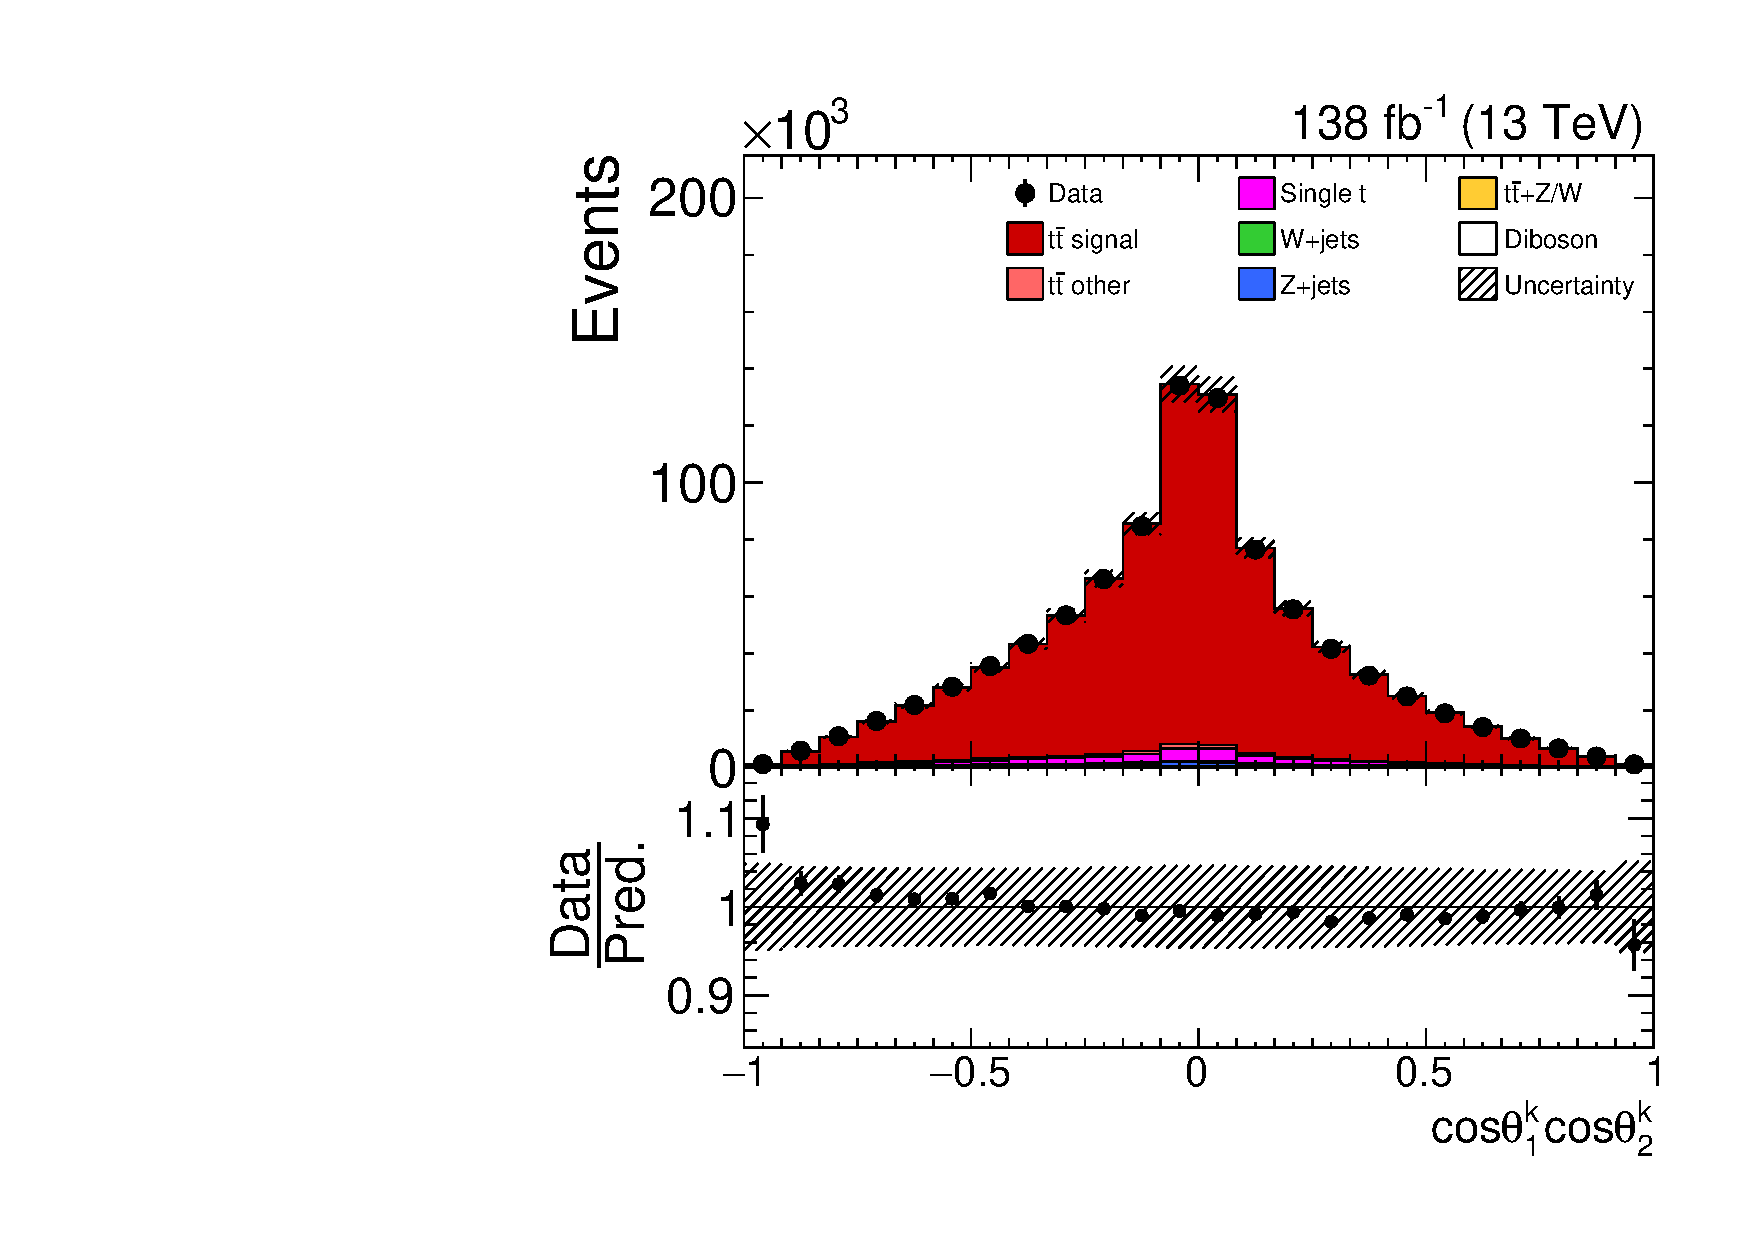
\includegraphics[width=0.40\textwidth]{fig_fullRun2UL/controlplots/combined/Hyp_LLBarCkk.pdf}
 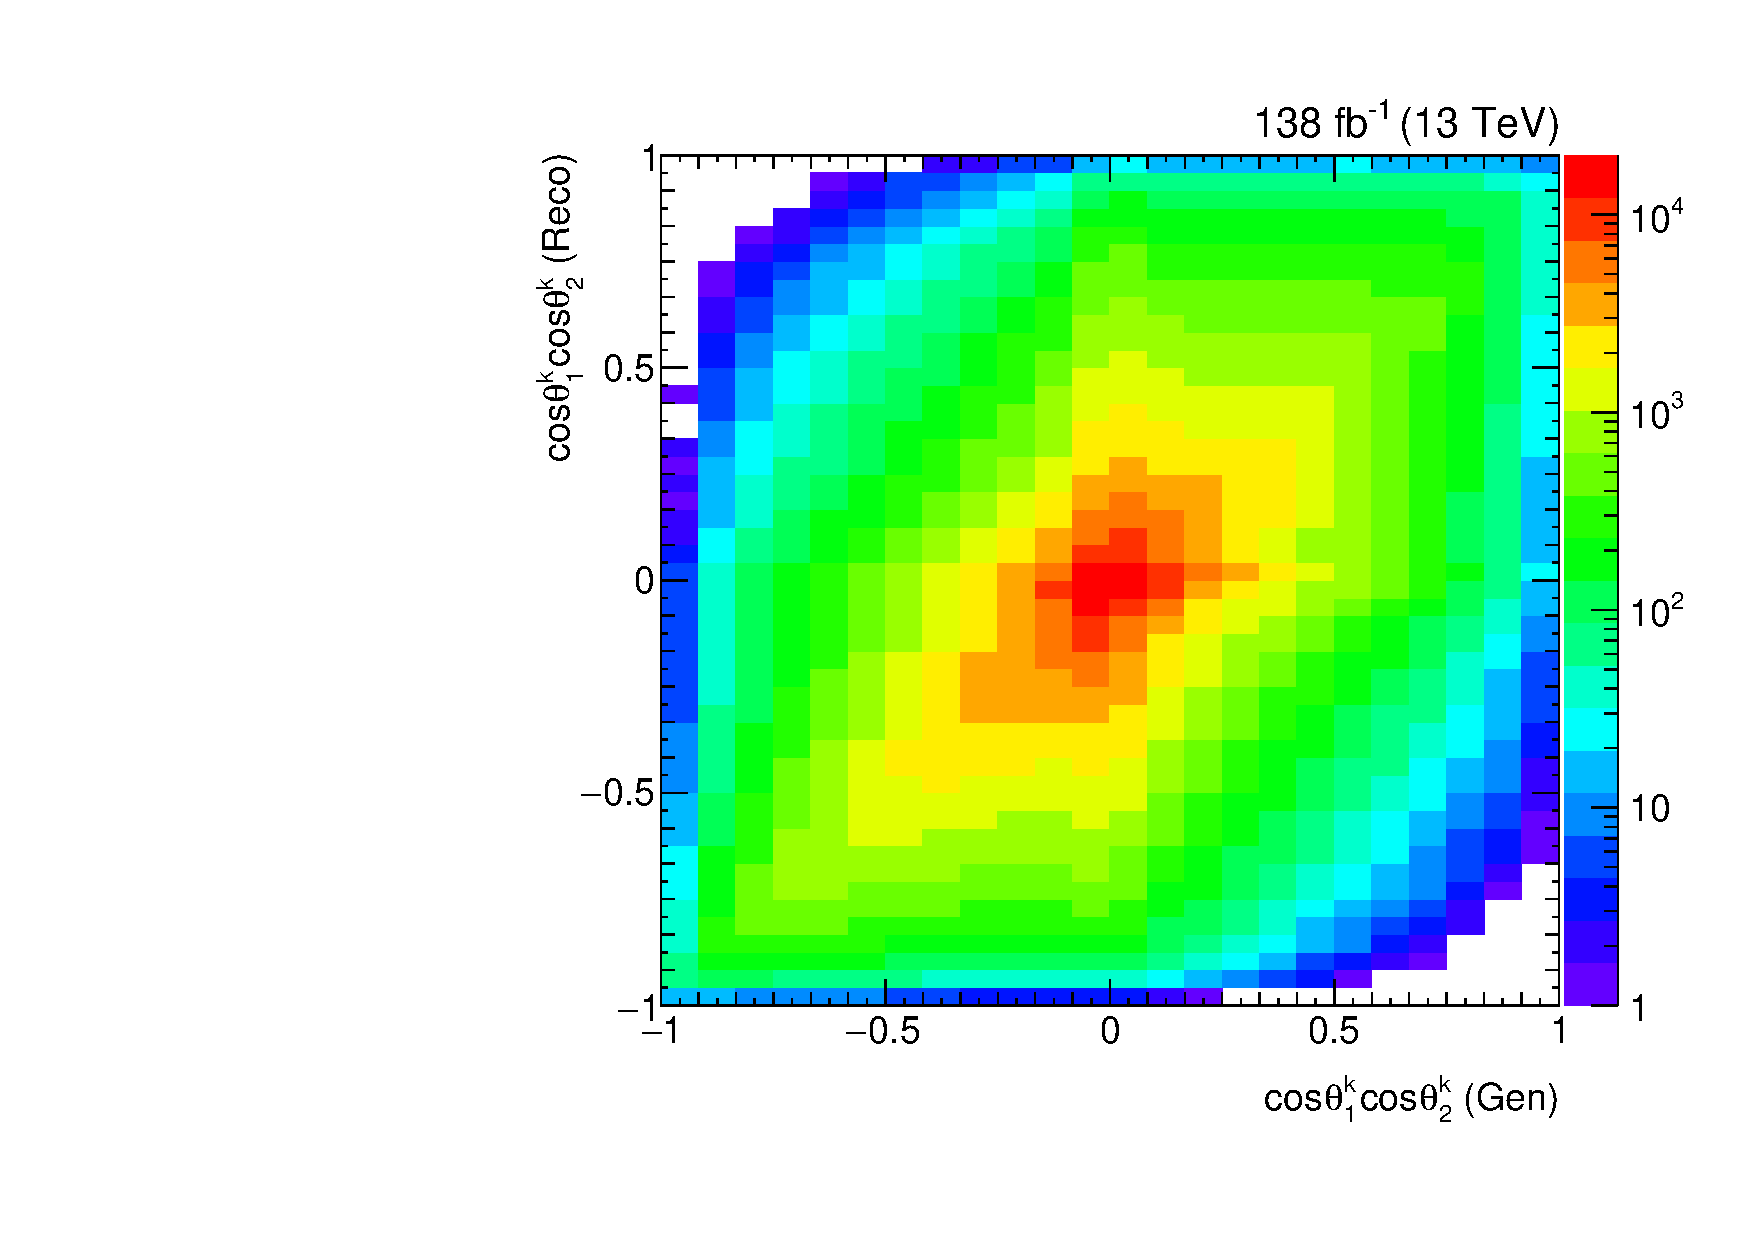
\includegraphics[width=0.40\textwidth]{fig_fullRun2UL/unfolding/combined/ResponseMatrix_c_kk.pdf} \\
 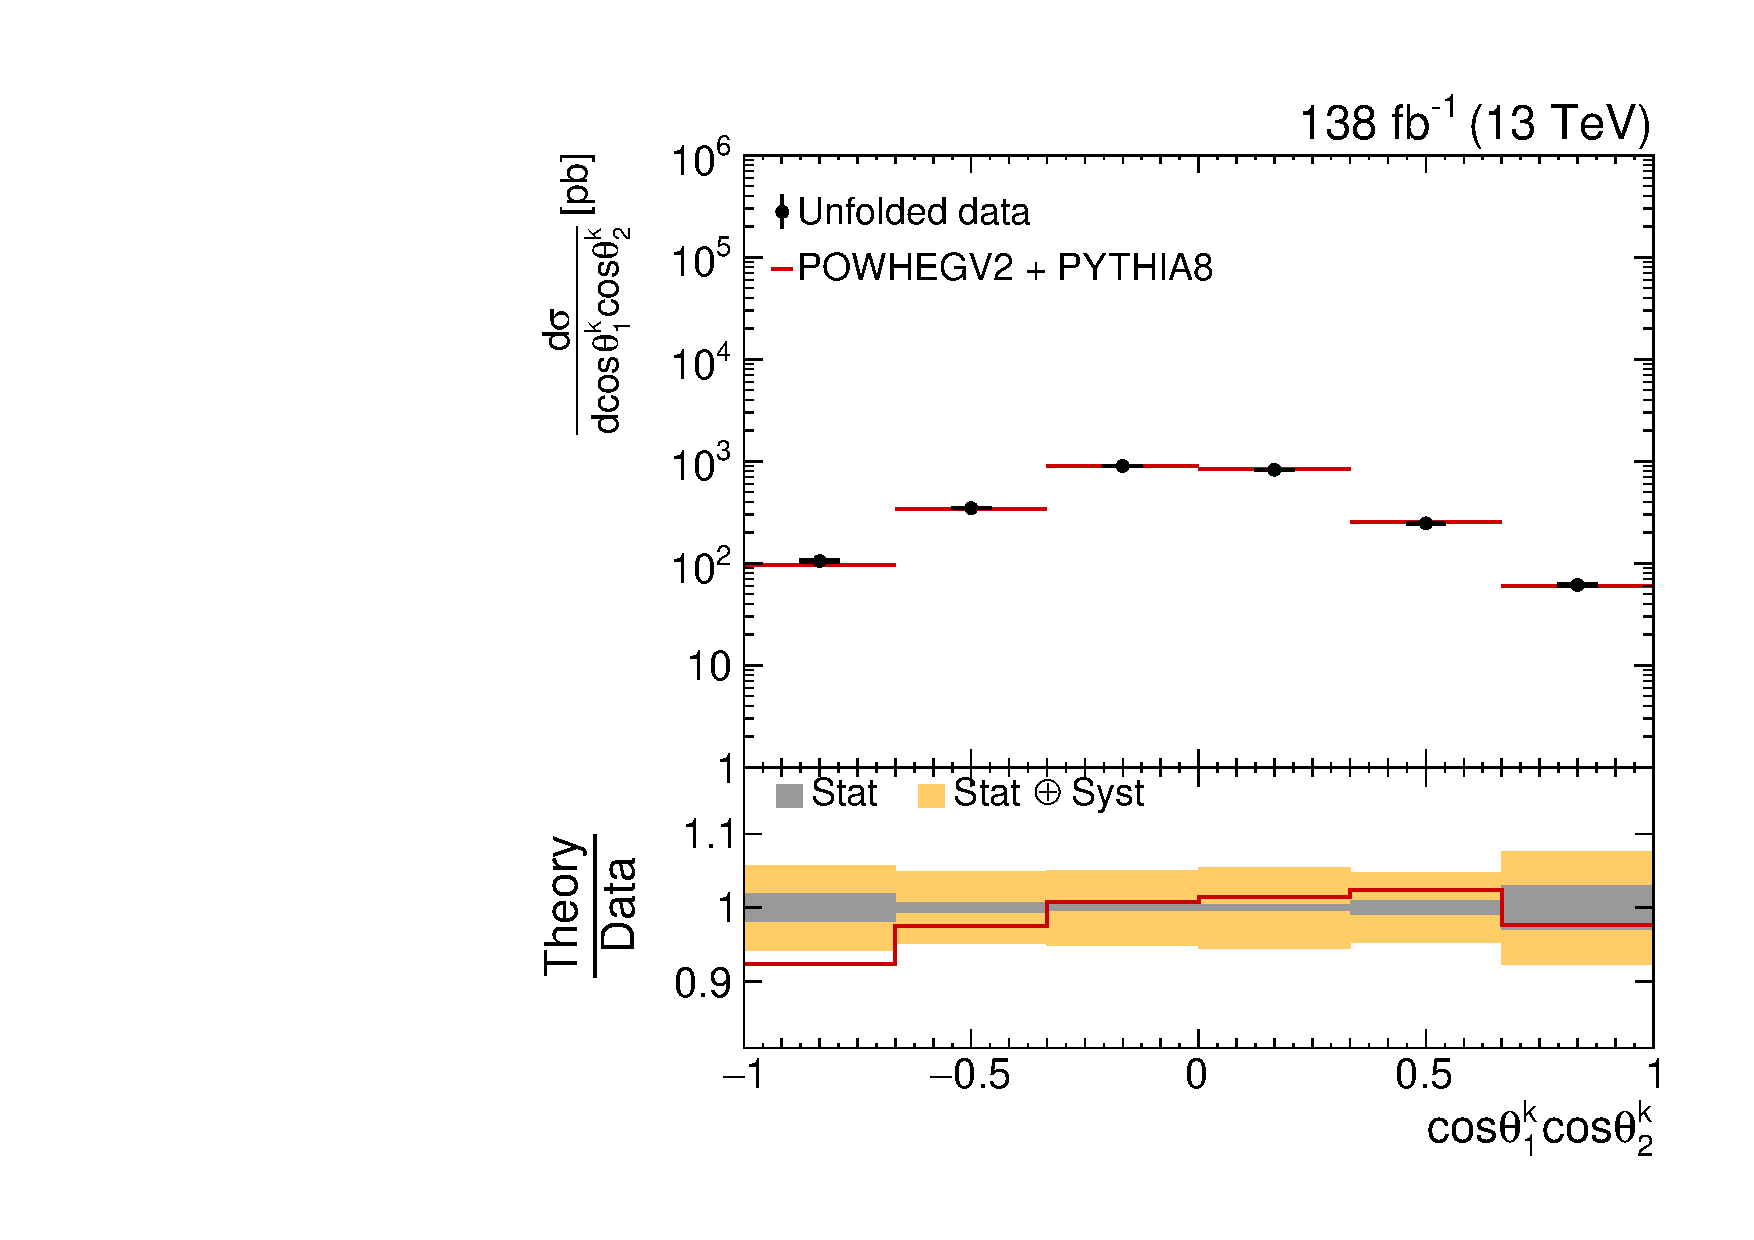
\includegraphics[width=0.40\textwidth]{fig_fullRun2UL/unfolding/combined/UnfoldedResults_c_kk.pdf}
 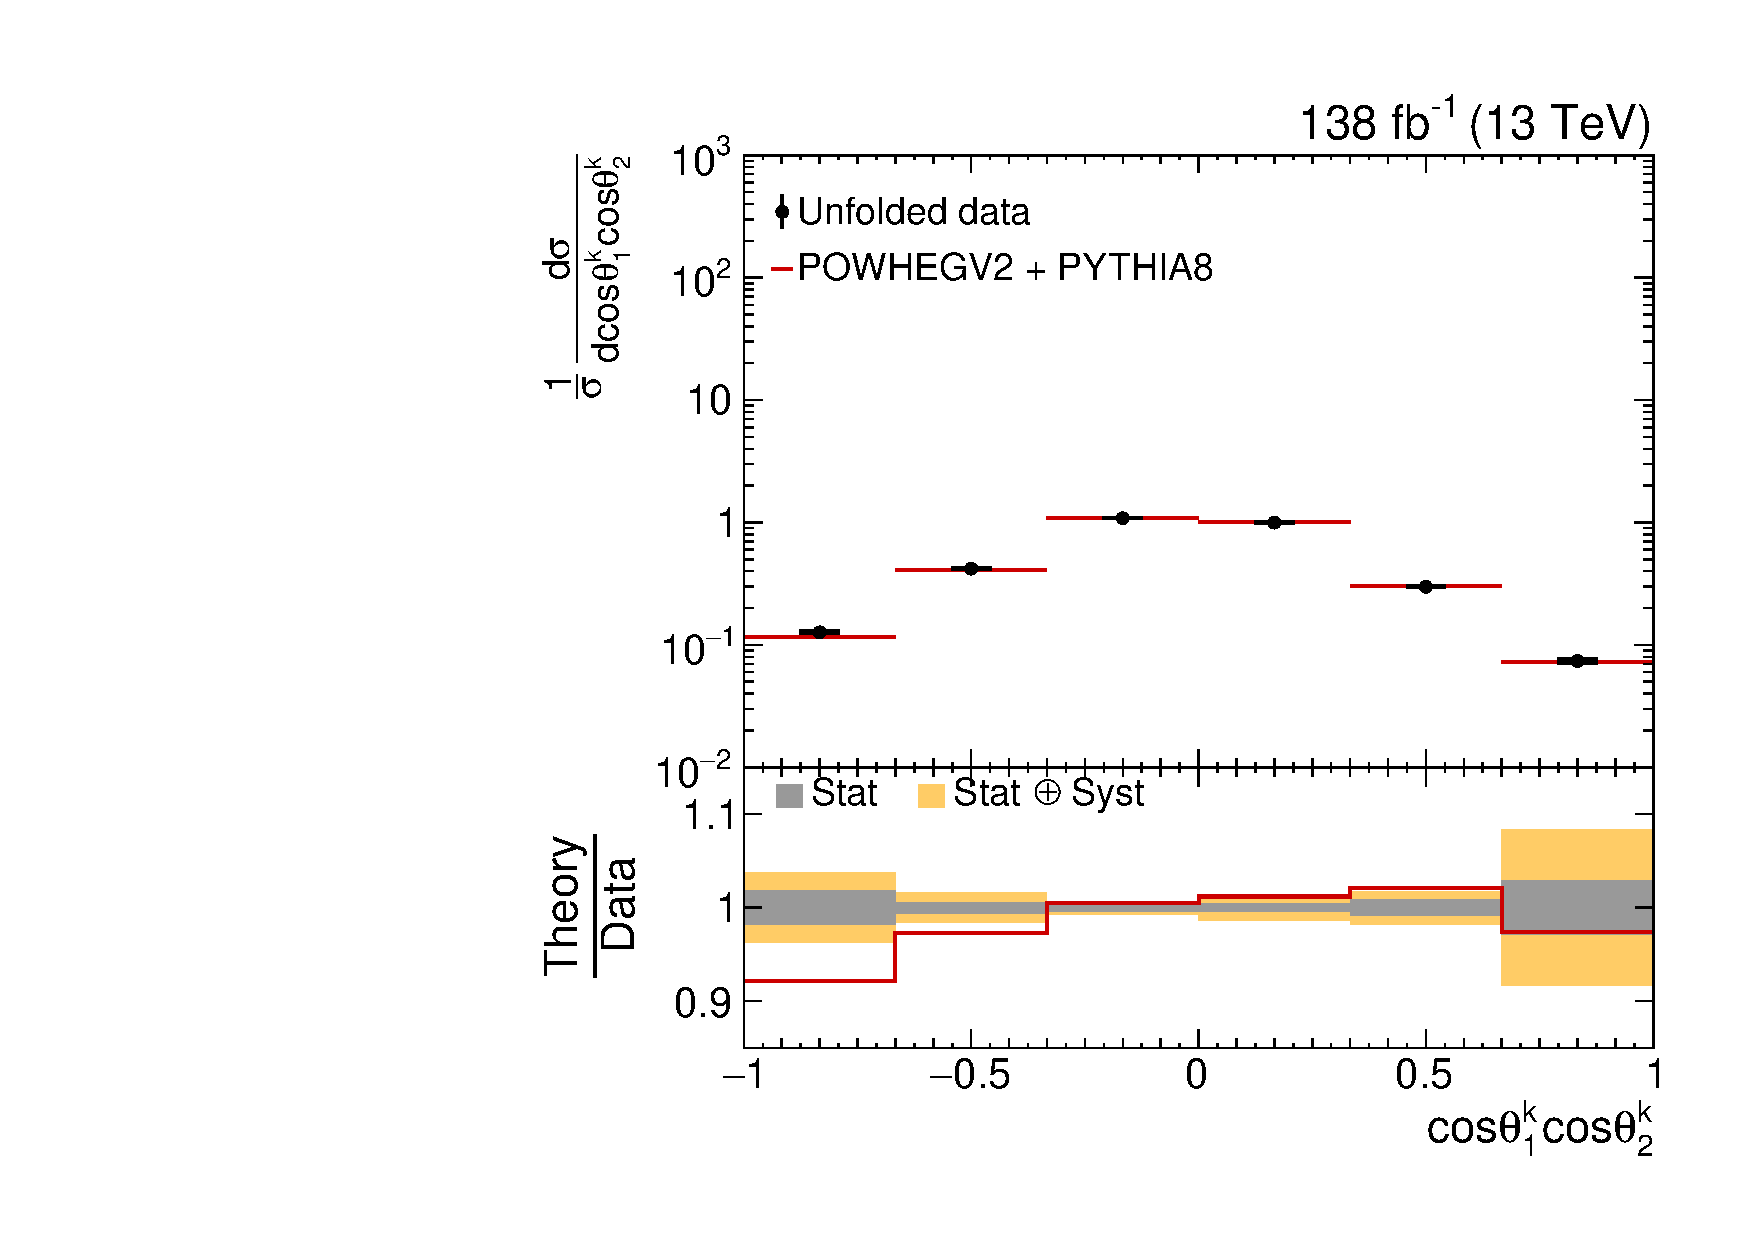
\includegraphics[width=0.40\textwidth]{fig_fullRun2UL/unfolding/combined/UnfoldedResultsNorm_c_kk.pdf} \\
\label{fig:c_kk}
\caption{Reconstructed detector-level distribution (Top Left), detector response-matrix (Top Right), absolute cross-section unfolded to parton-level (Bottom Left), and normalized cross-section unfolded to parton-level (Bottom Right) for diagonal spin correlation observable $\cos\theta_{1}^{k}\cos\theta_{2}^{k}$, from which spin-density coefficient $C_{kk}$ (sensitive to spin-density coefficient function $c_{k k}$) is extracted.}
\end{center}
\end{figure}
\clearpage
\begin{figure}[htb]
\begin{center}
 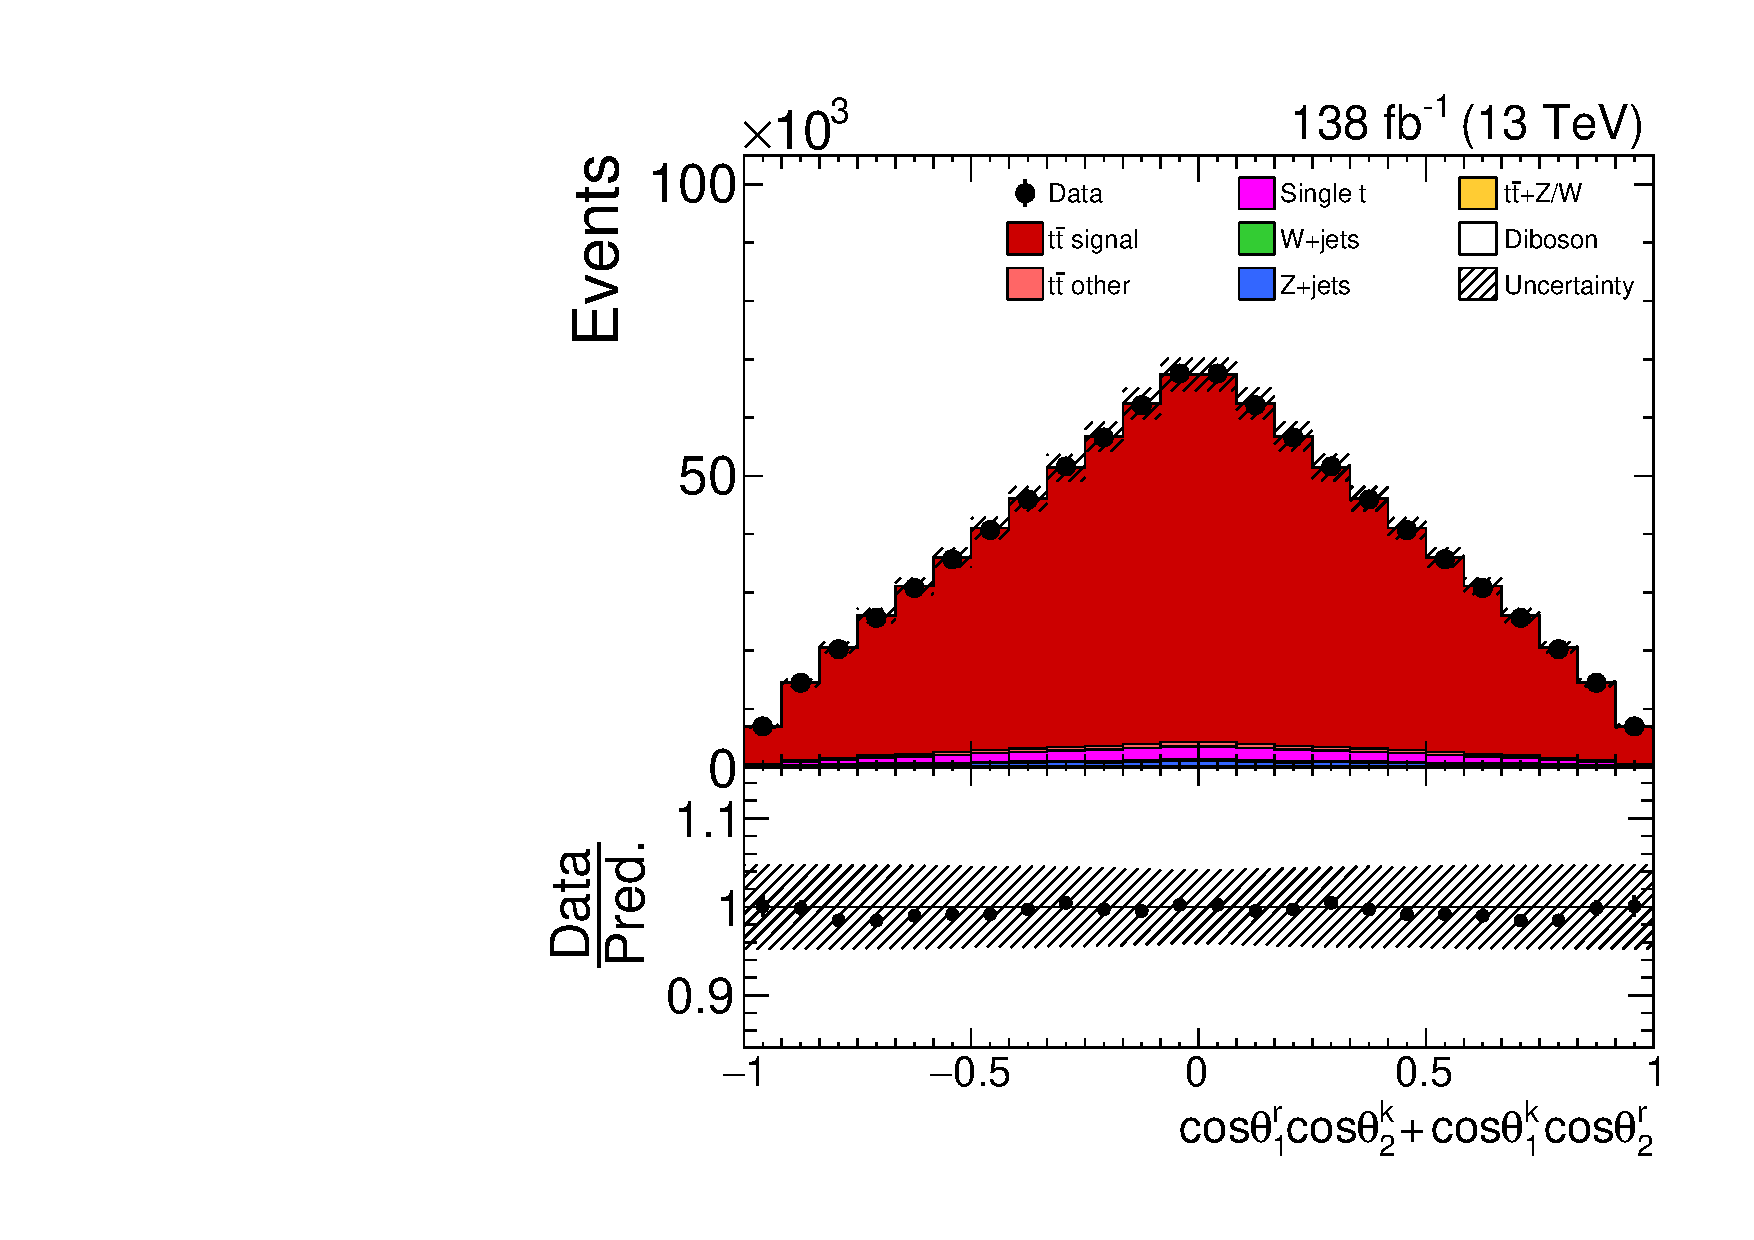
\includegraphics[width=0.40\textwidth]{fig_fullRun2UL/controlplots/combined/Hyp_LLBarCPrk.pdf}
 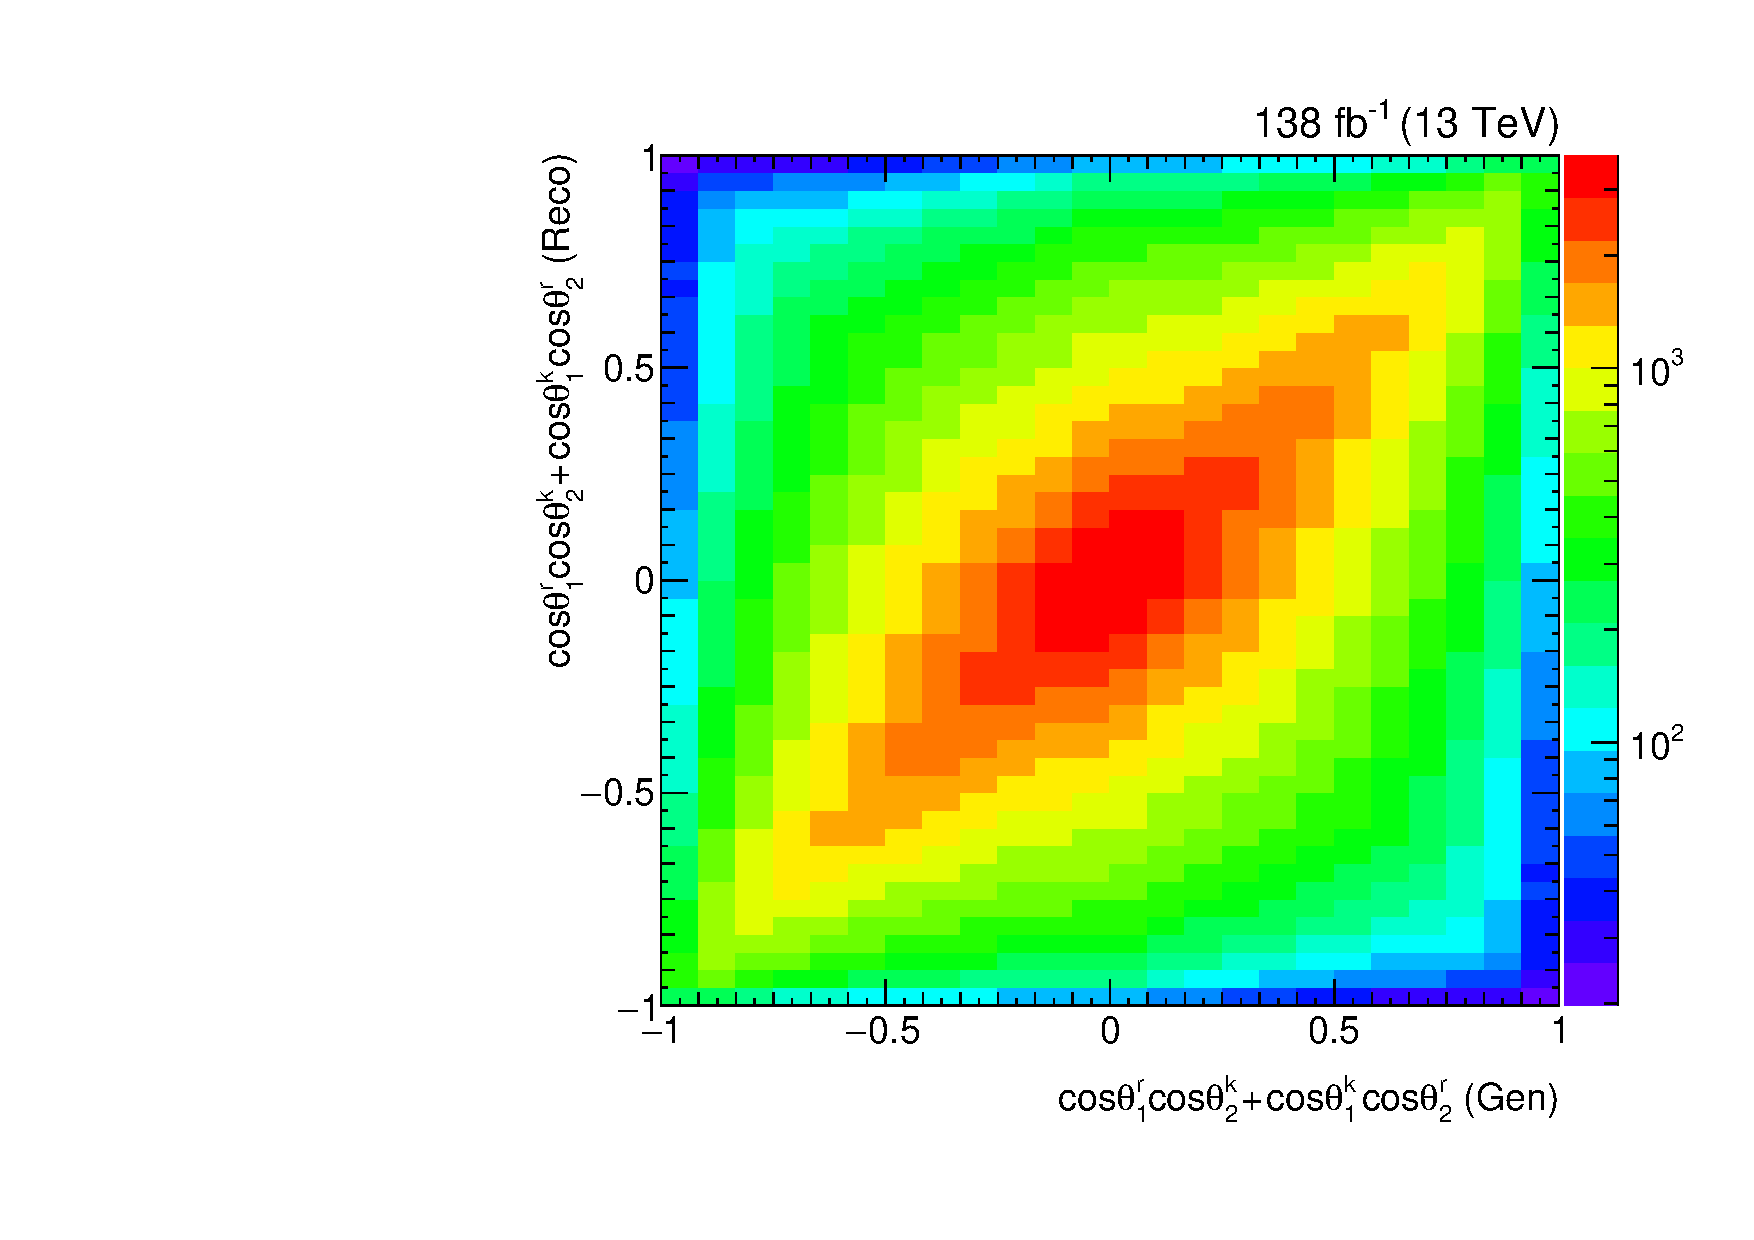
\includegraphics[width=0.40\textwidth]{fig_fullRun2UL/unfolding/combined/ResponseMatrix_c_Prk.pdf} \\
 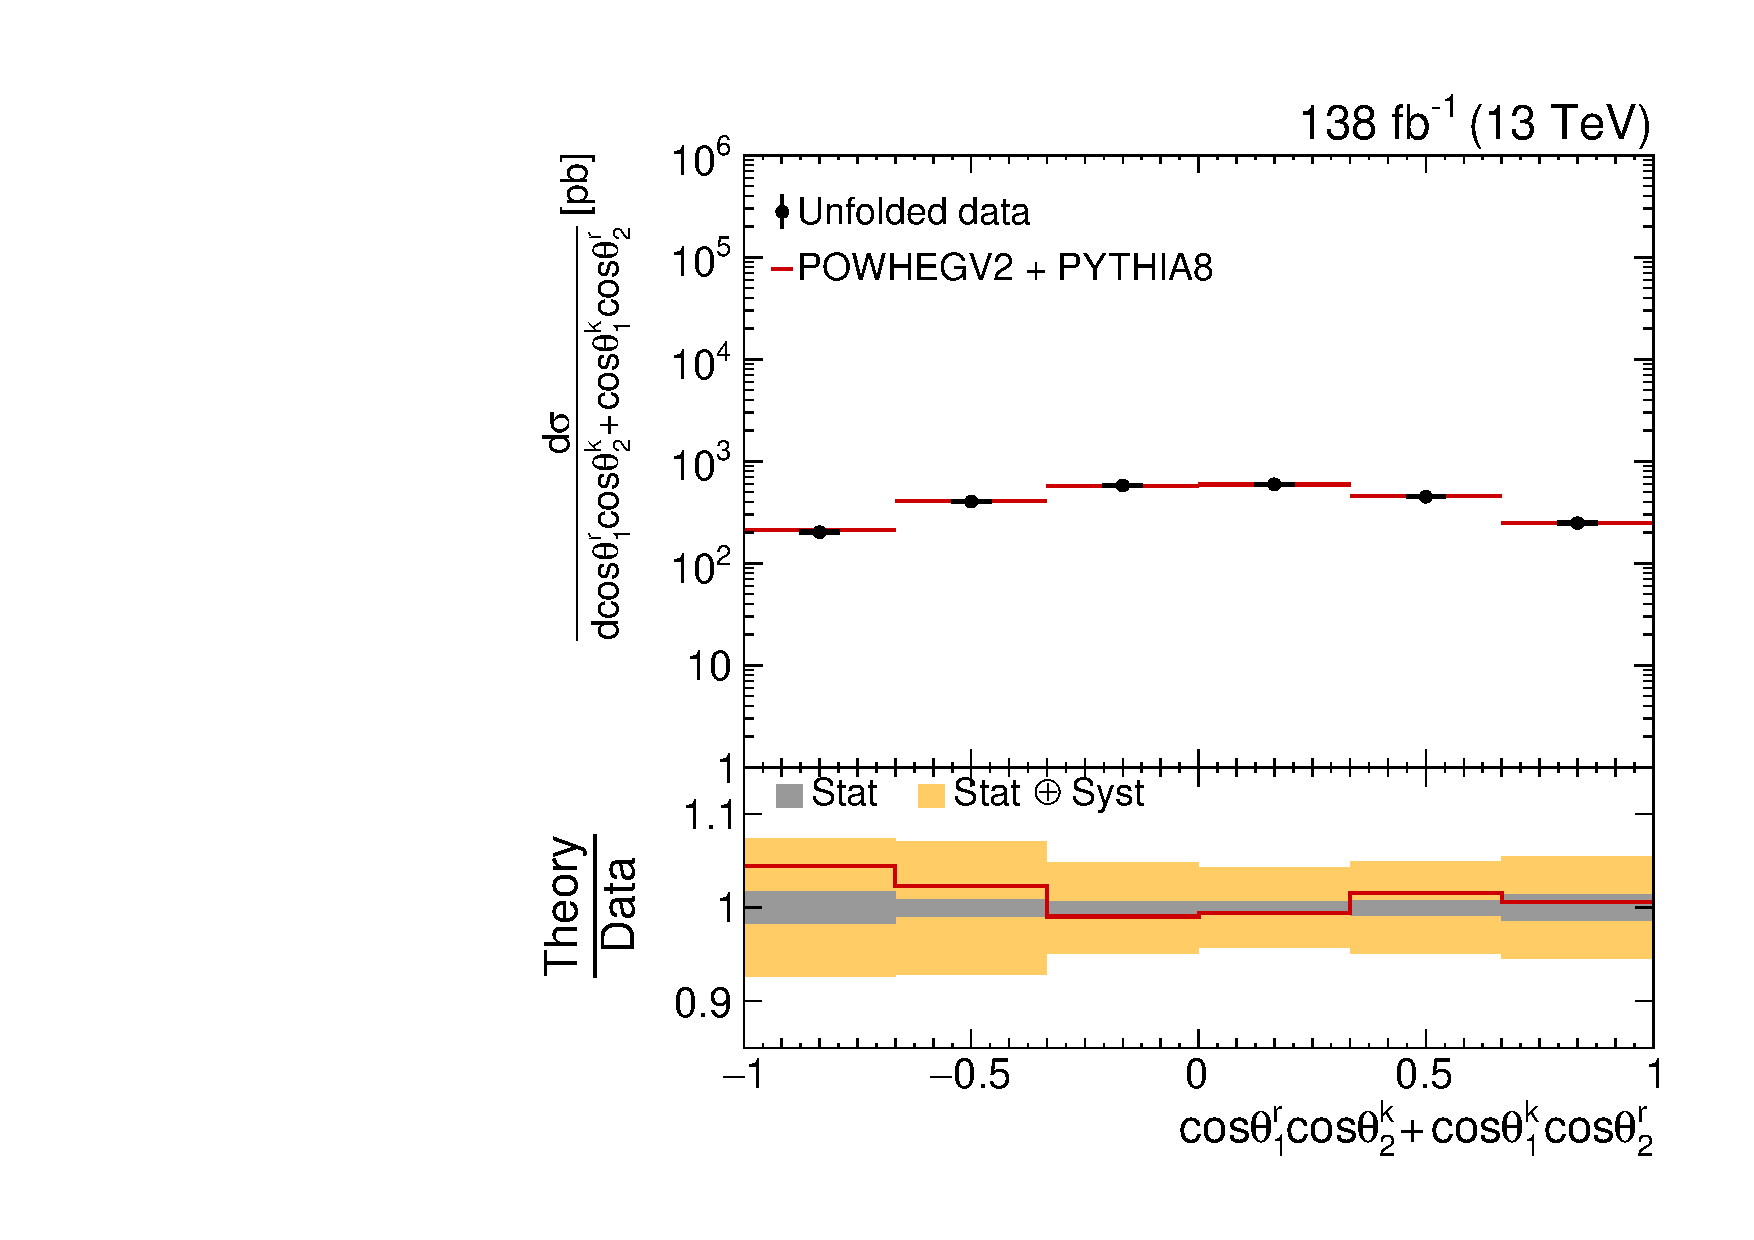
\includegraphics[width=0.40\textwidth]{fig_fullRun2UL/unfolding/combined/UnfoldedResults_c_Prk.pdf}
 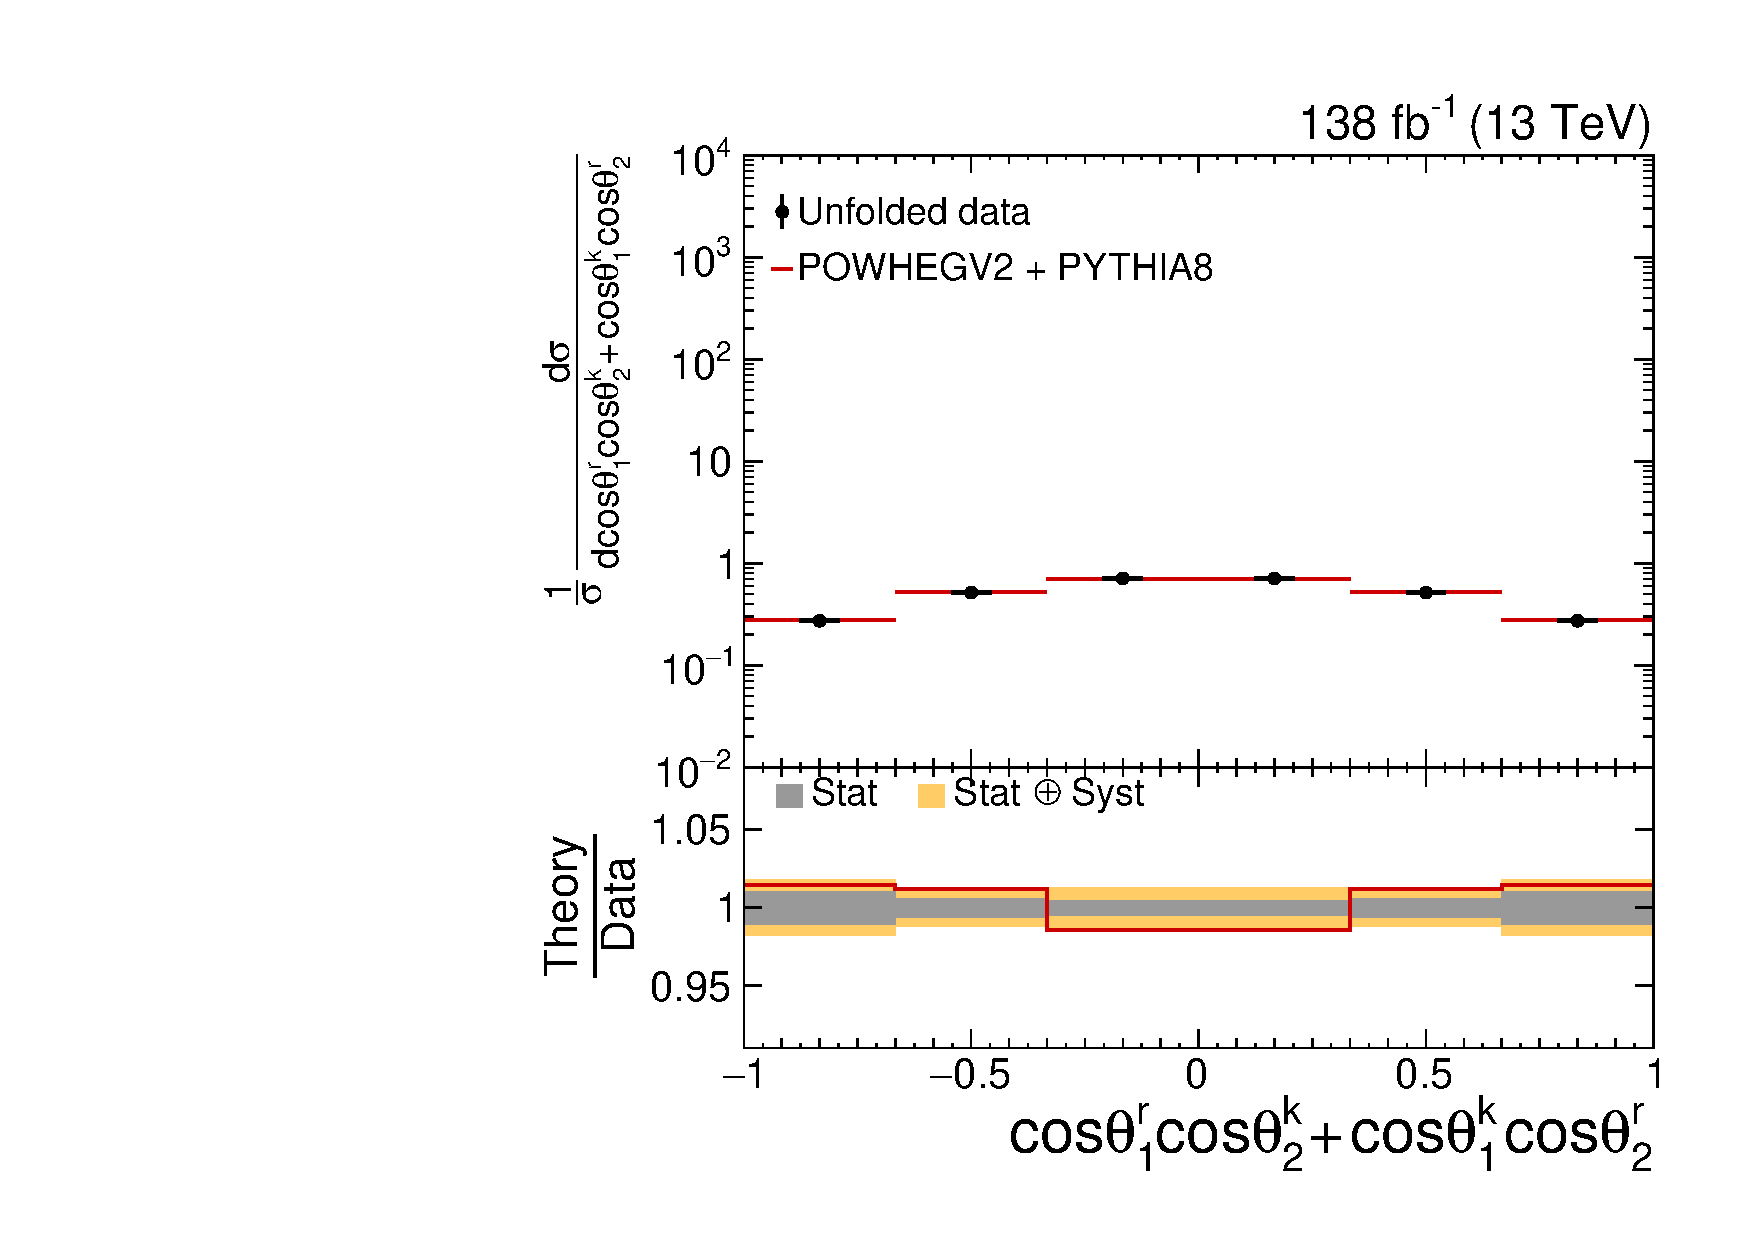
\includegraphics[width=0.40\textwidth]{fig_fullRun2UL/unfolding/combined/UnfoldedResultsNorm_c_Prk.pdf} \\
\label{fig:c_Prk}
\caption{Reconstructed detector-level distribution (Top Left), detector response-matrix (Top Right), absolute cross-section unfolded to parton-level (Bottom Left), and normalized cross-section unfolded to parton-level (Bottom Right) for off-diagonal spin correlation sum observable $\cos\theta_{1}^{r}\cos\theta_{2}^{k}+\cos\theta_{1}^{k}\cos\theta_{2}^{r}$, from which spin-density coefficient $C_{rk}+C_{kr}$ (sensitive to spin-density coefficient function $c_{r k}$) is extracted.}
\end{center}
\end{figure}
\clearpage
\begin{figure}[htb]
\begin{center}
 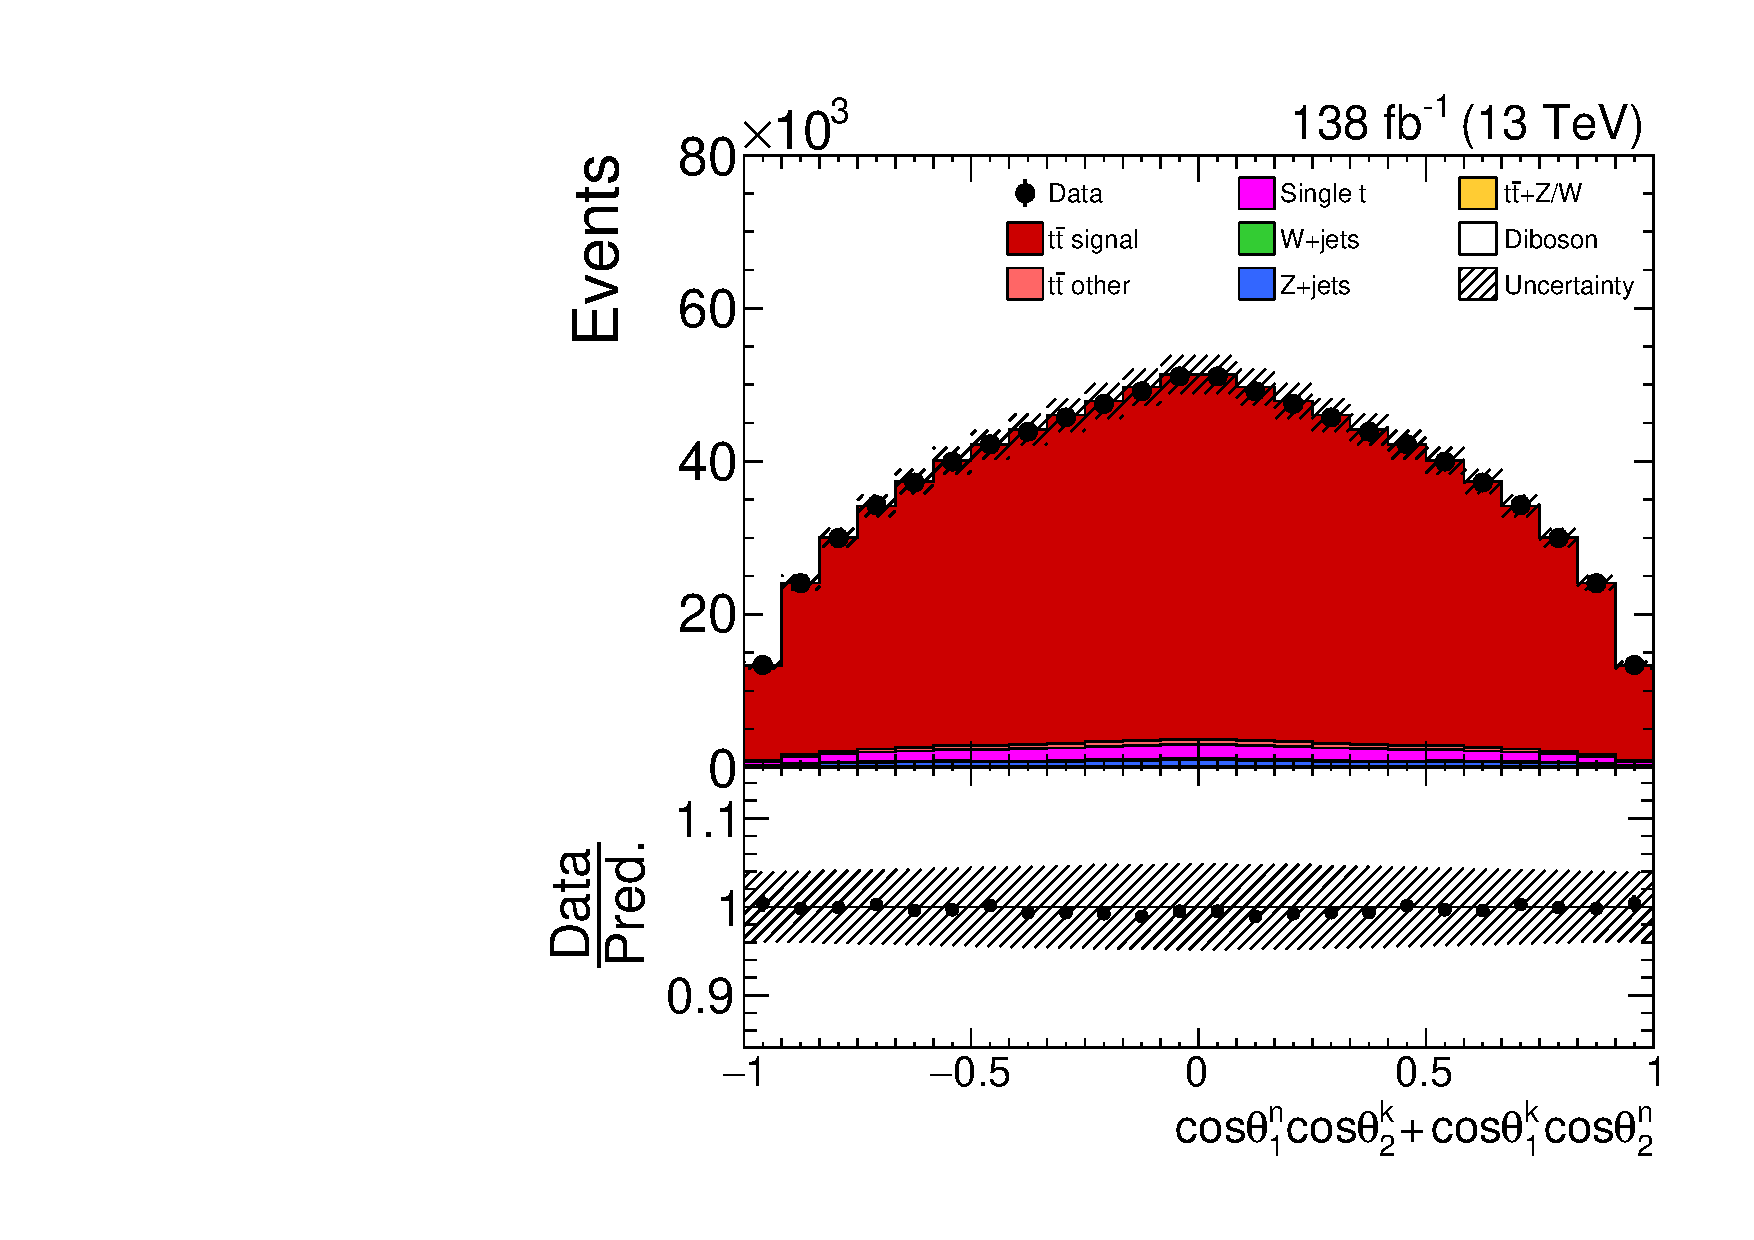
\includegraphics[width=0.40\textwidth]{fig_fullRun2UL/controlplots/combined/Hyp_LLBarCPnk.pdf}
 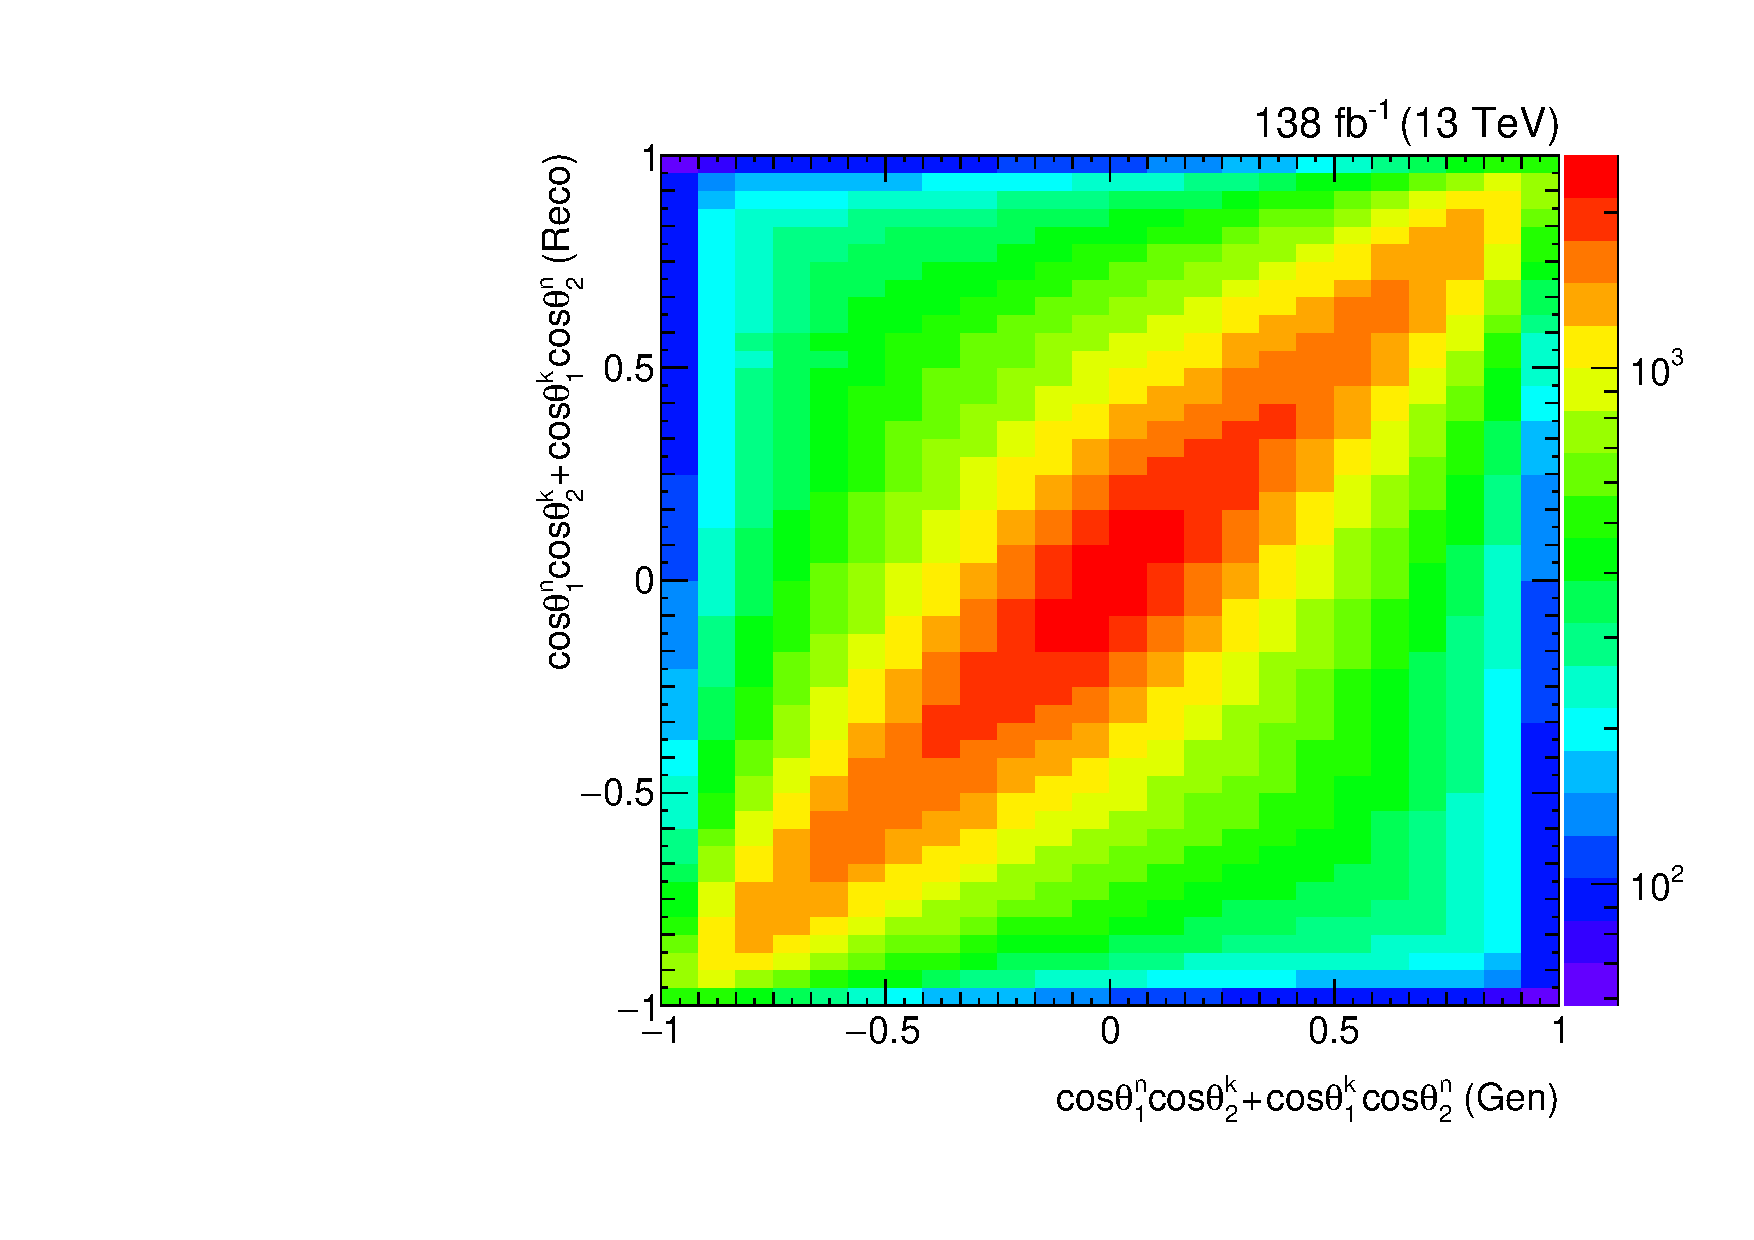
\includegraphics[width=0.40\textwidth]{fig_fullRun2UL/unfolding/combined/ResponseMatrix_c_Pnk.pdf} \\
 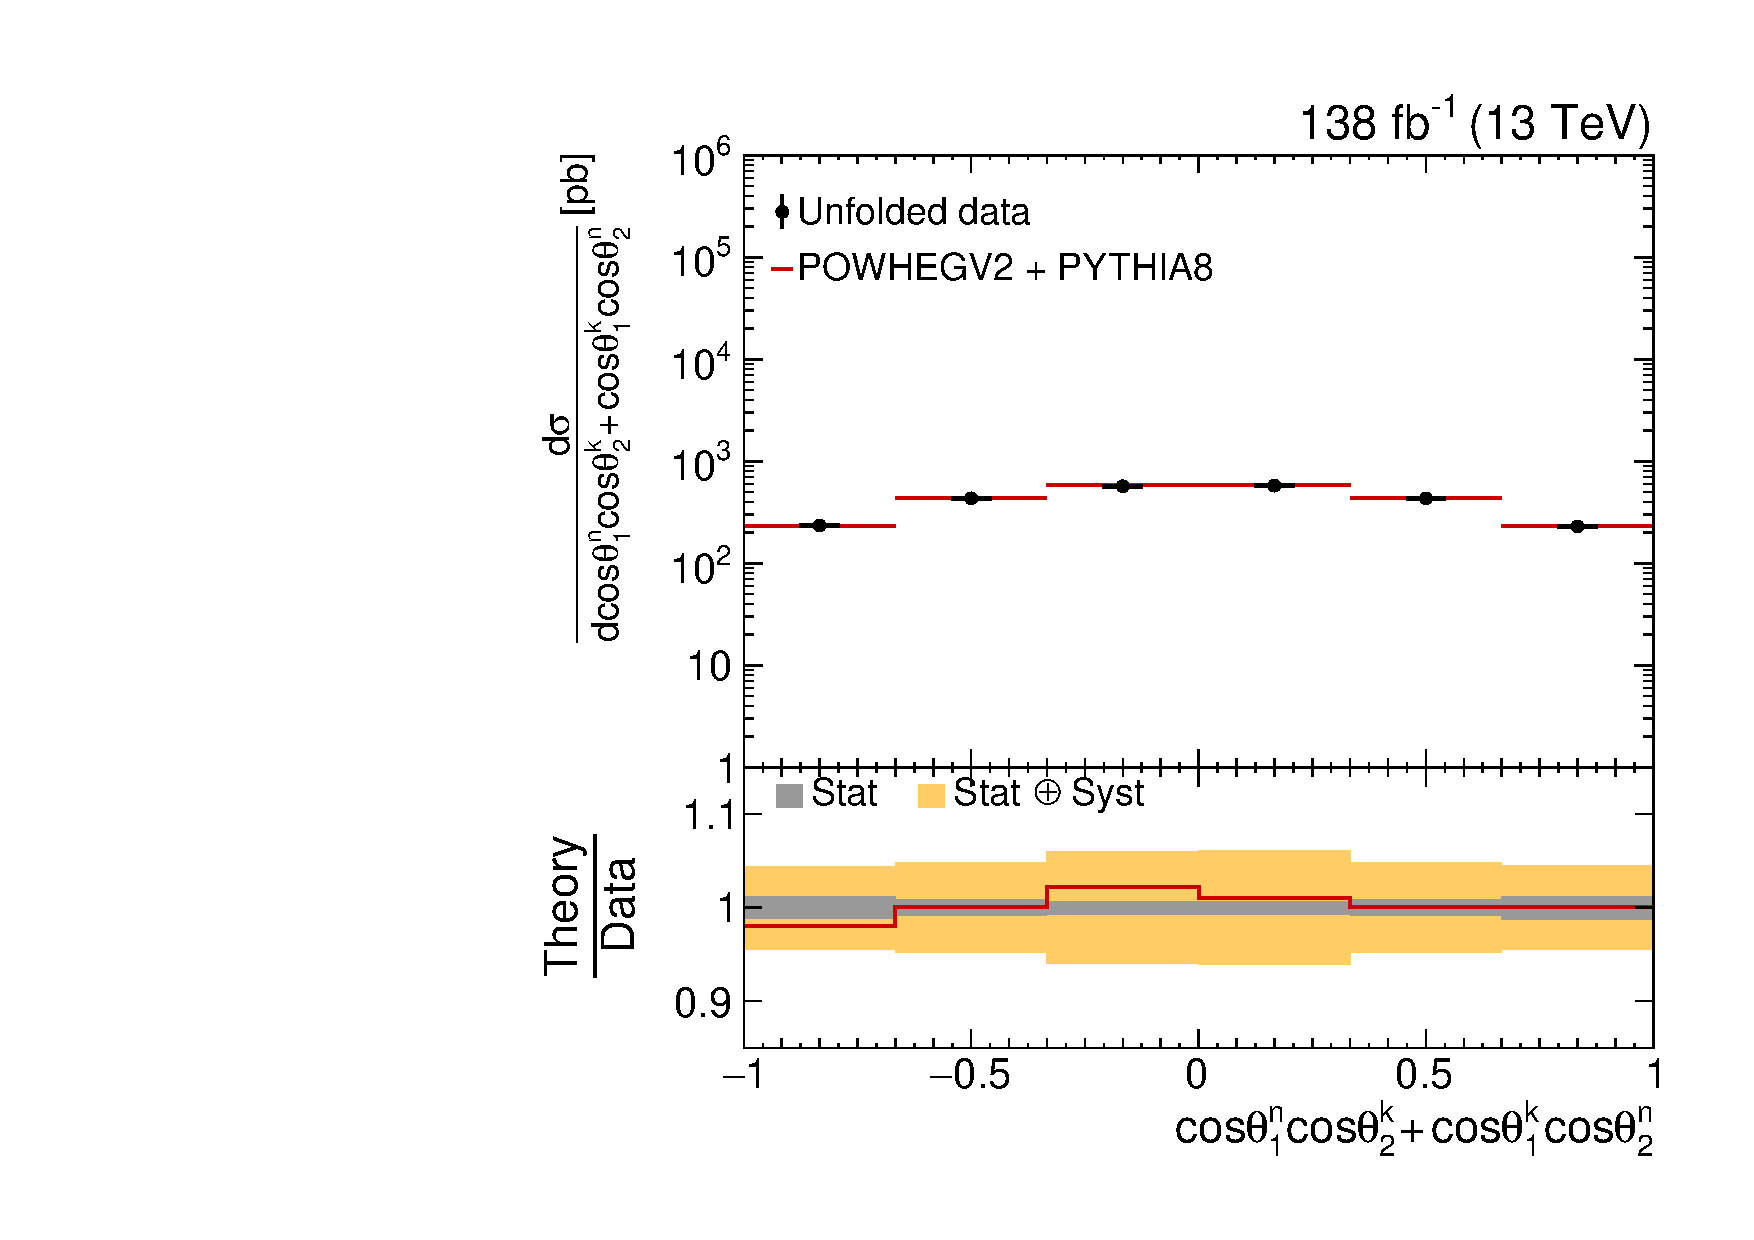
\includegraphics[width=0.40\textwidth]{fig_fullRun2UL/unfolding/combined/UnfoldedResults_c_Pnk.pdf}
 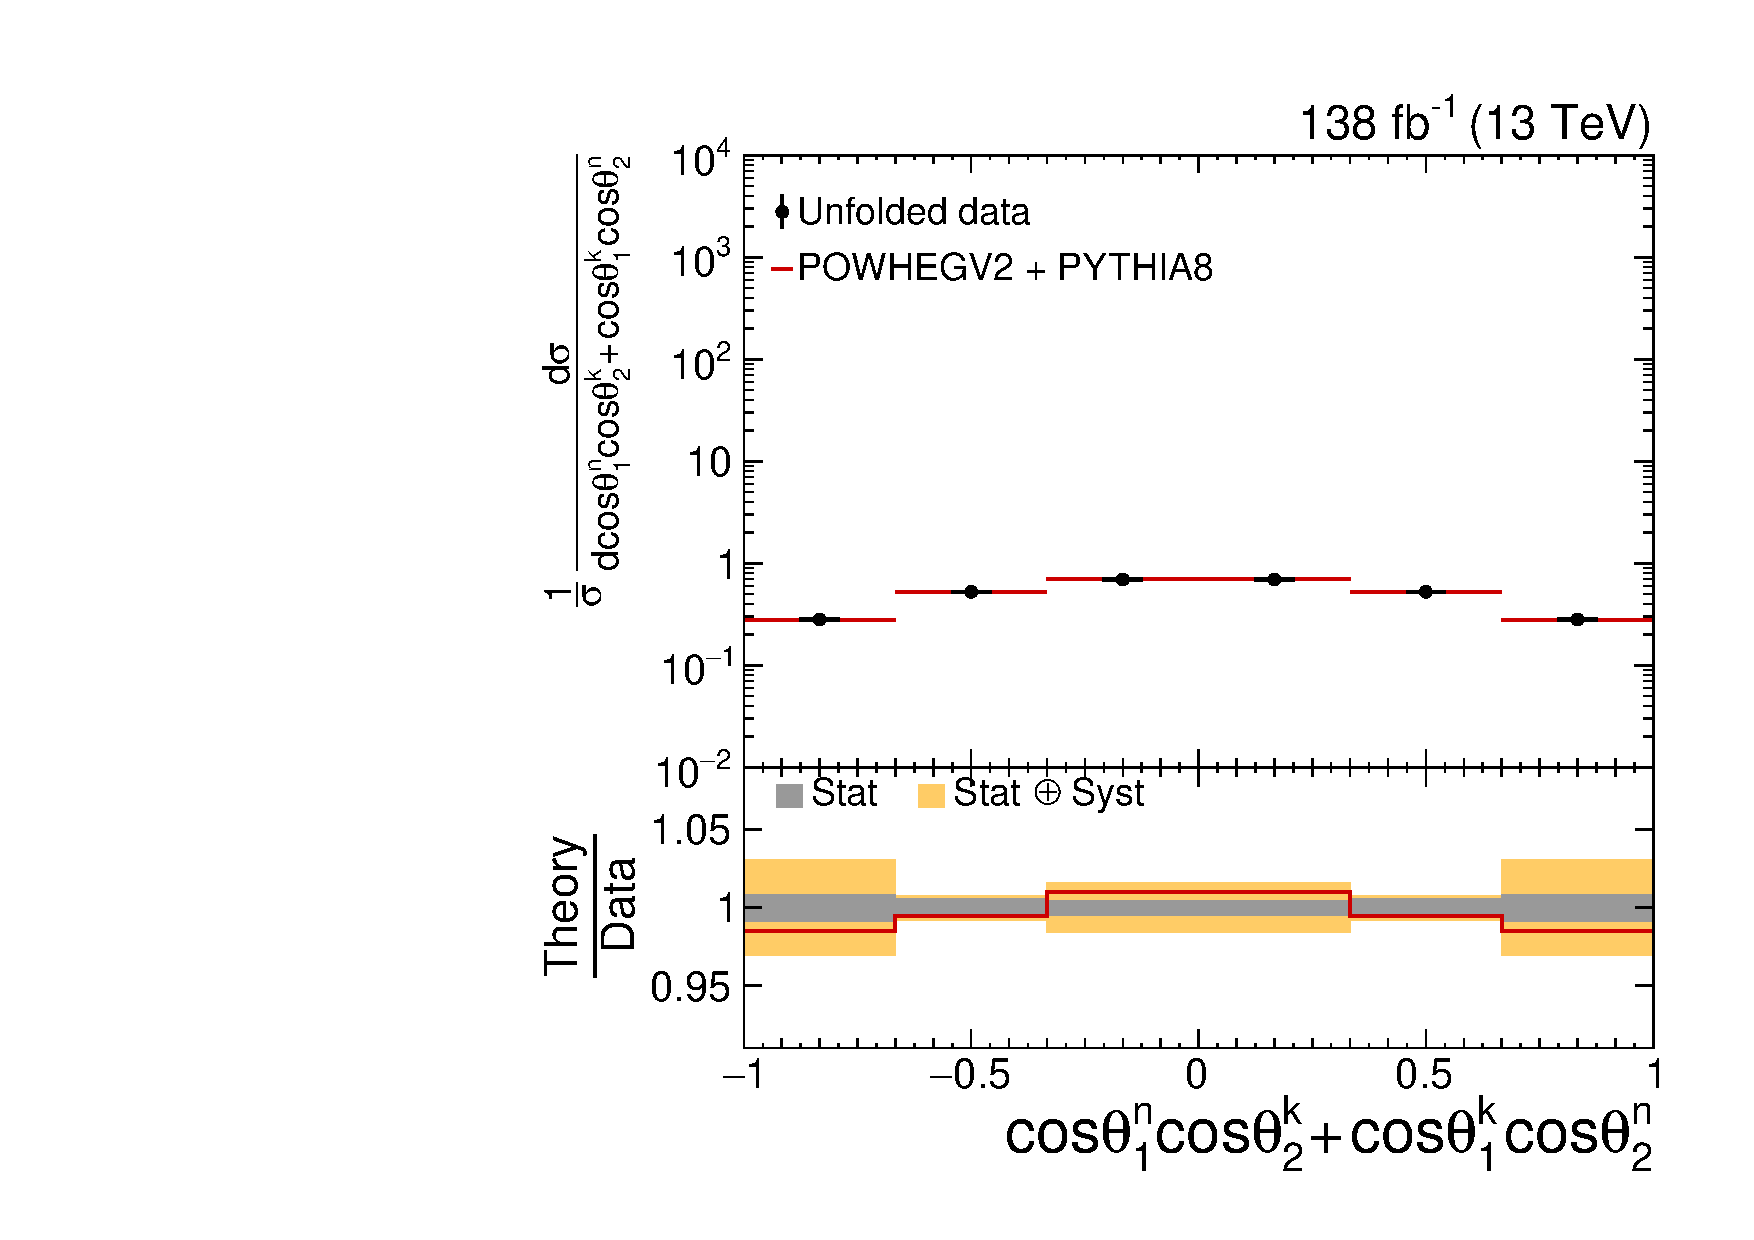
\includegraphics[width=0.40\textwidth]{fig_fullRun2UL/unfolding/combined/UnfoldedResultsNorm_c_Pnk.pdf} \\
\label{fig:c_Pnk}
\caption{Reconstructed detector-level distribution (Top Left), detector response-matrix (Top Right), absolute cross-section unfolded to parton-level (Bottom Left), and normalized cross-section unfolded to parton-level (Bottom Right) for off-diagonal spin correlation sum observable $\cos\theta_{1}^{n}\cos\theta_{2}^{k}+\cos\theta_{1}^{k}\cos\theta_{2}^{n}$, from which spin-density coefficient $C_{nk}+C_{kn}$ (sensitive to spin-density coefficient function $c_{k n}$) is extracted.}
\end{center}
\end{figure}
\clearpage
\begin{figure}[htb]
\begin{center}
 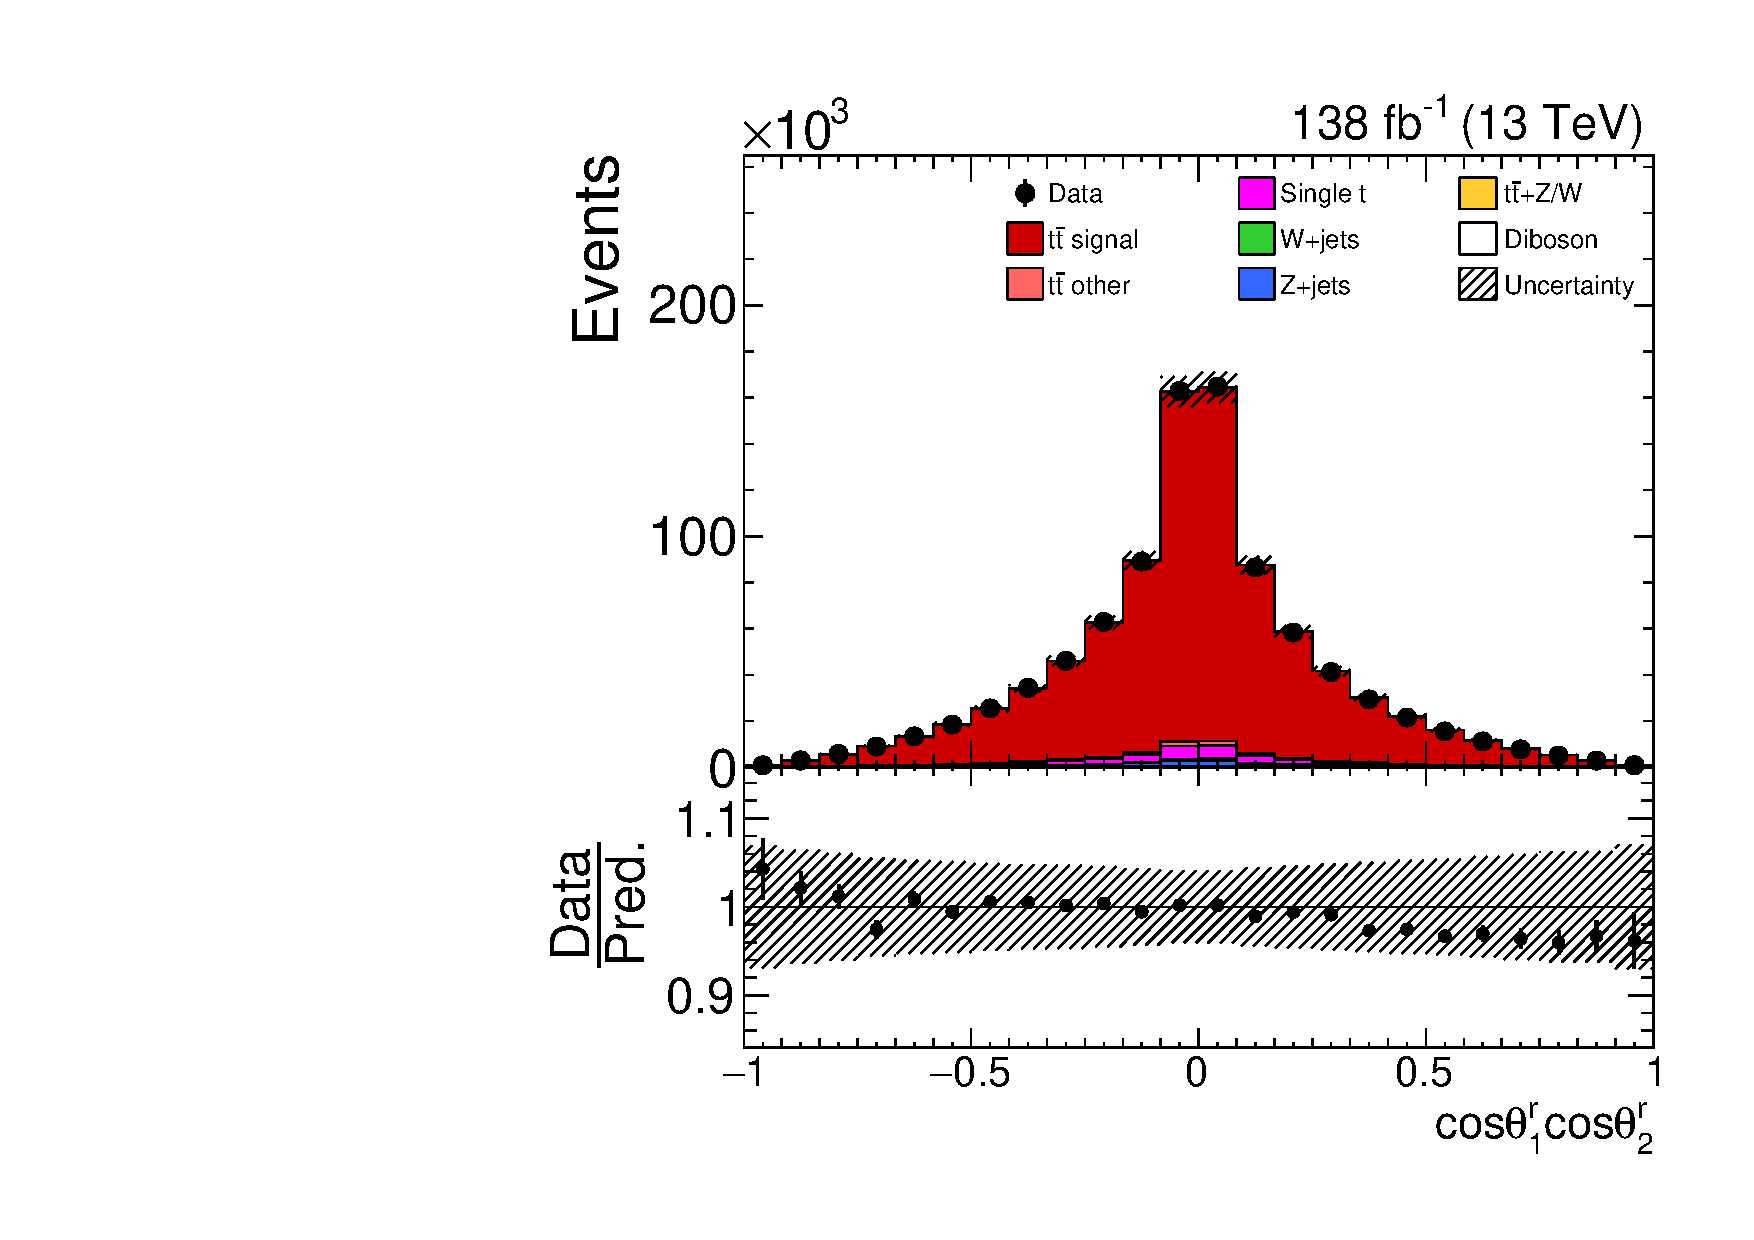
\includegraphics[width=0.40\textwidth]{fig_fullRun2UL/controlplots/combined/Hyp_LLBarCrr.pdf}
 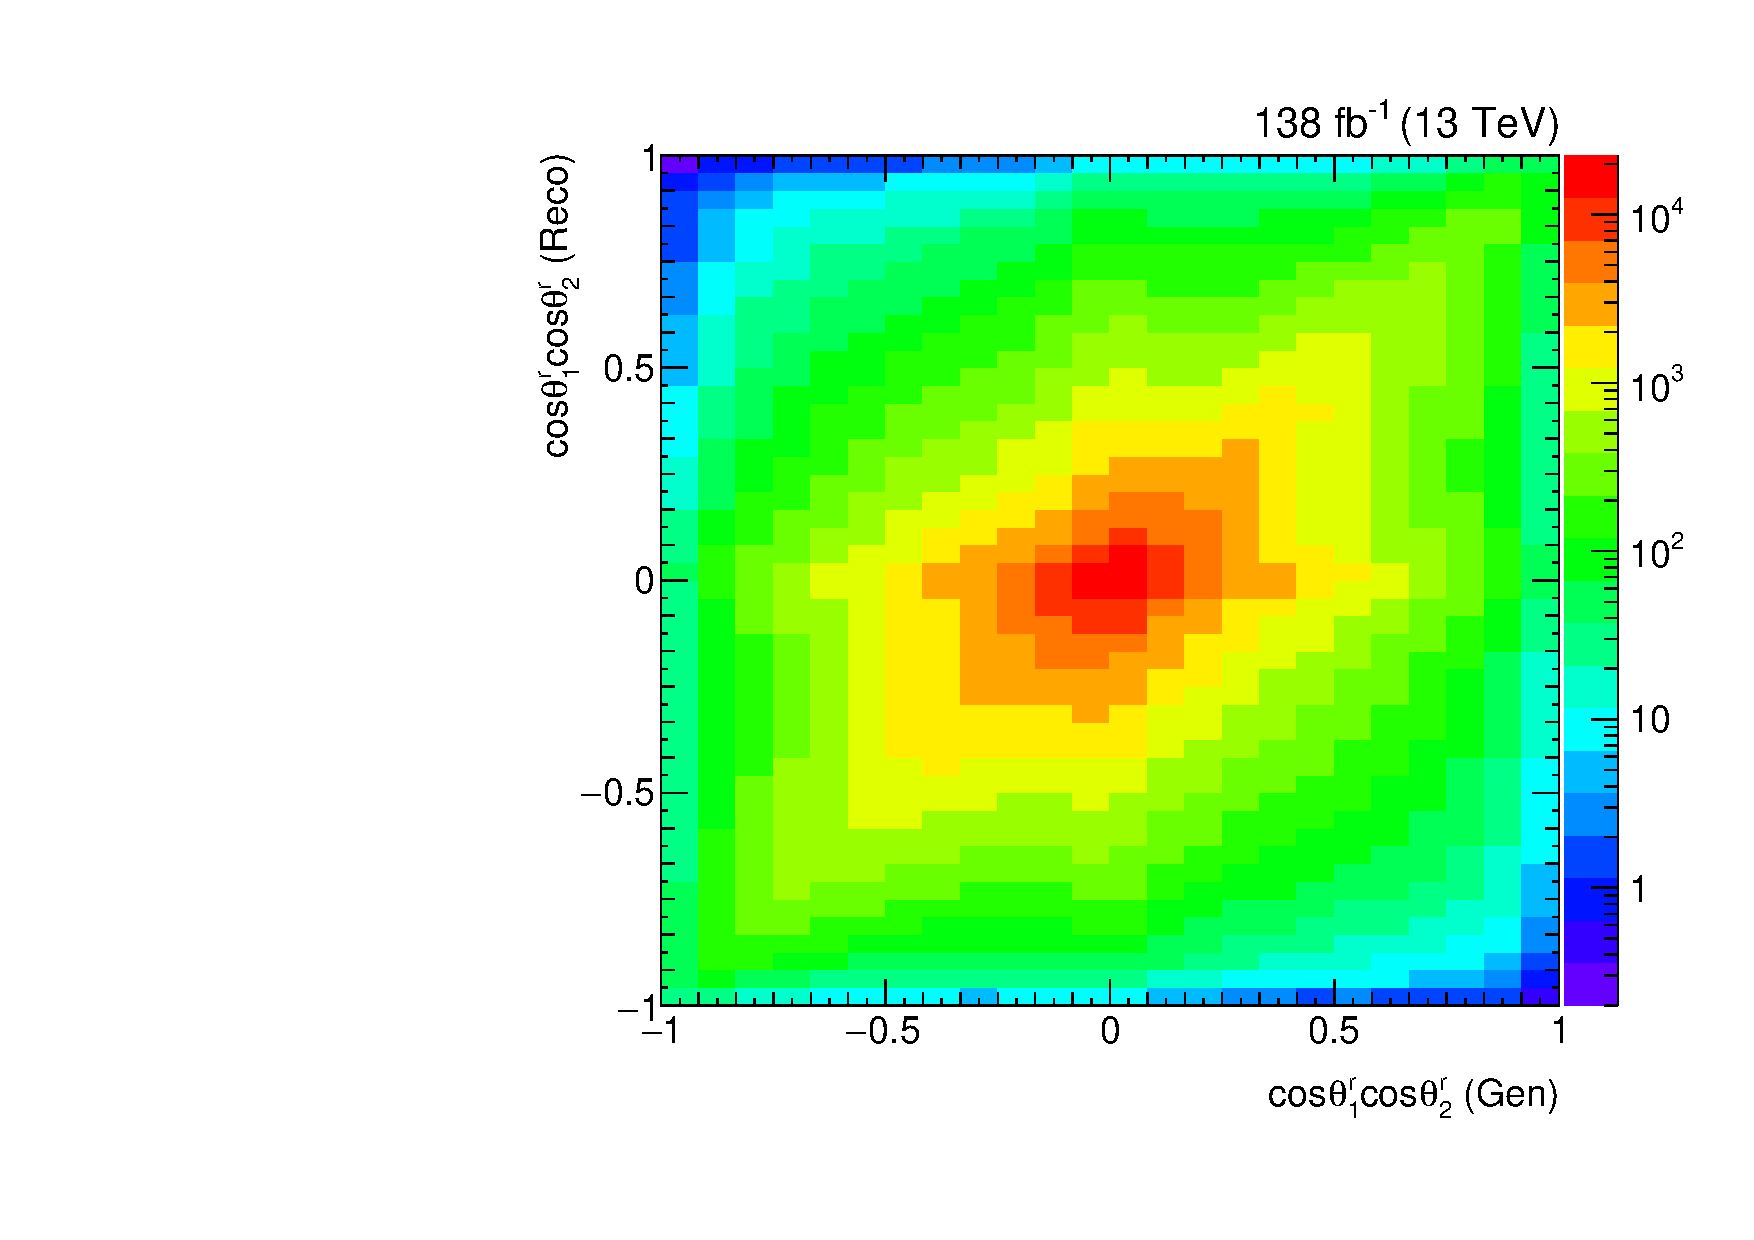
\includegraphics[width=0.40\textwidth]{fig_fullRun2UL/unfolding/combined/ResponseMatrix_c_rr.pdf} \\
 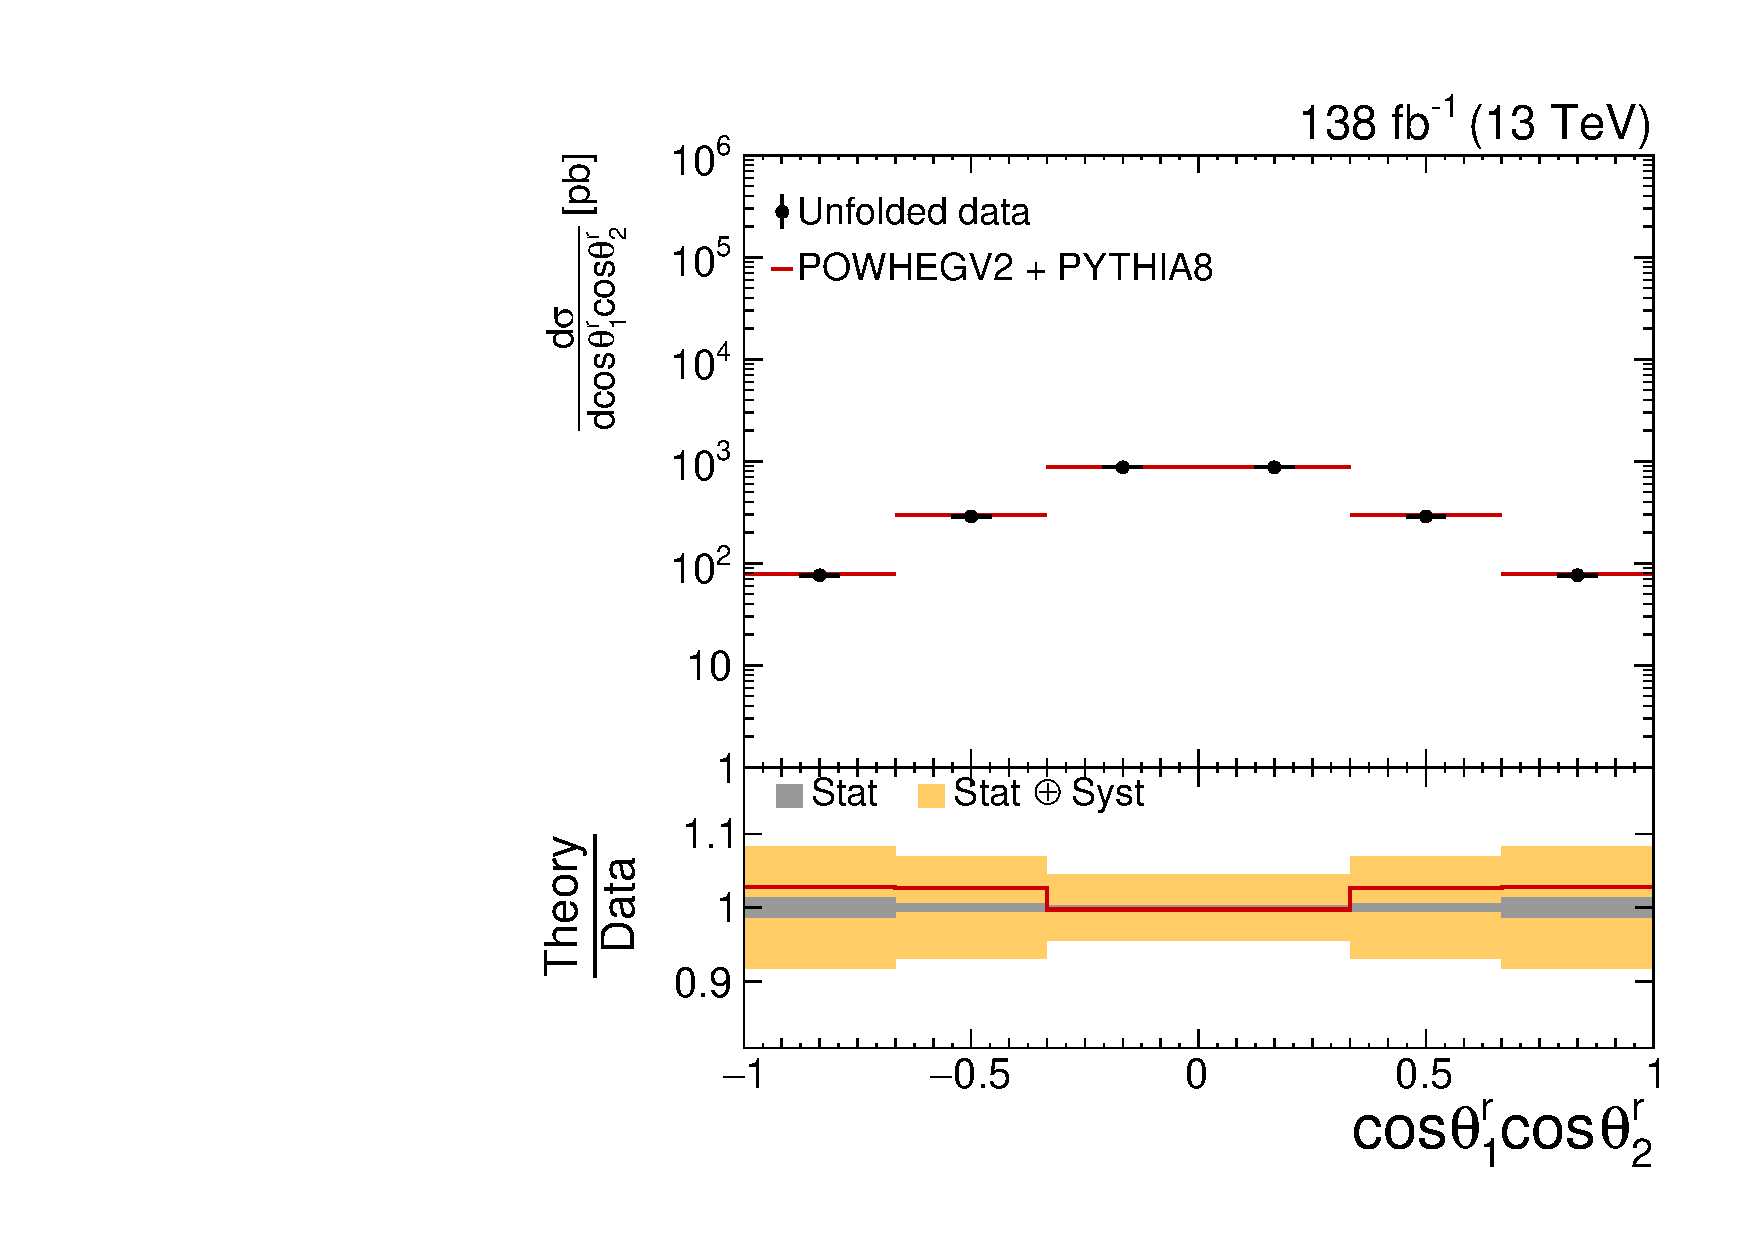
\includegraphics[width=0.40\textwidth]{fig_fullRun2UL/unfolding/combined/UnfoldedResults_c_rr.pdf}
 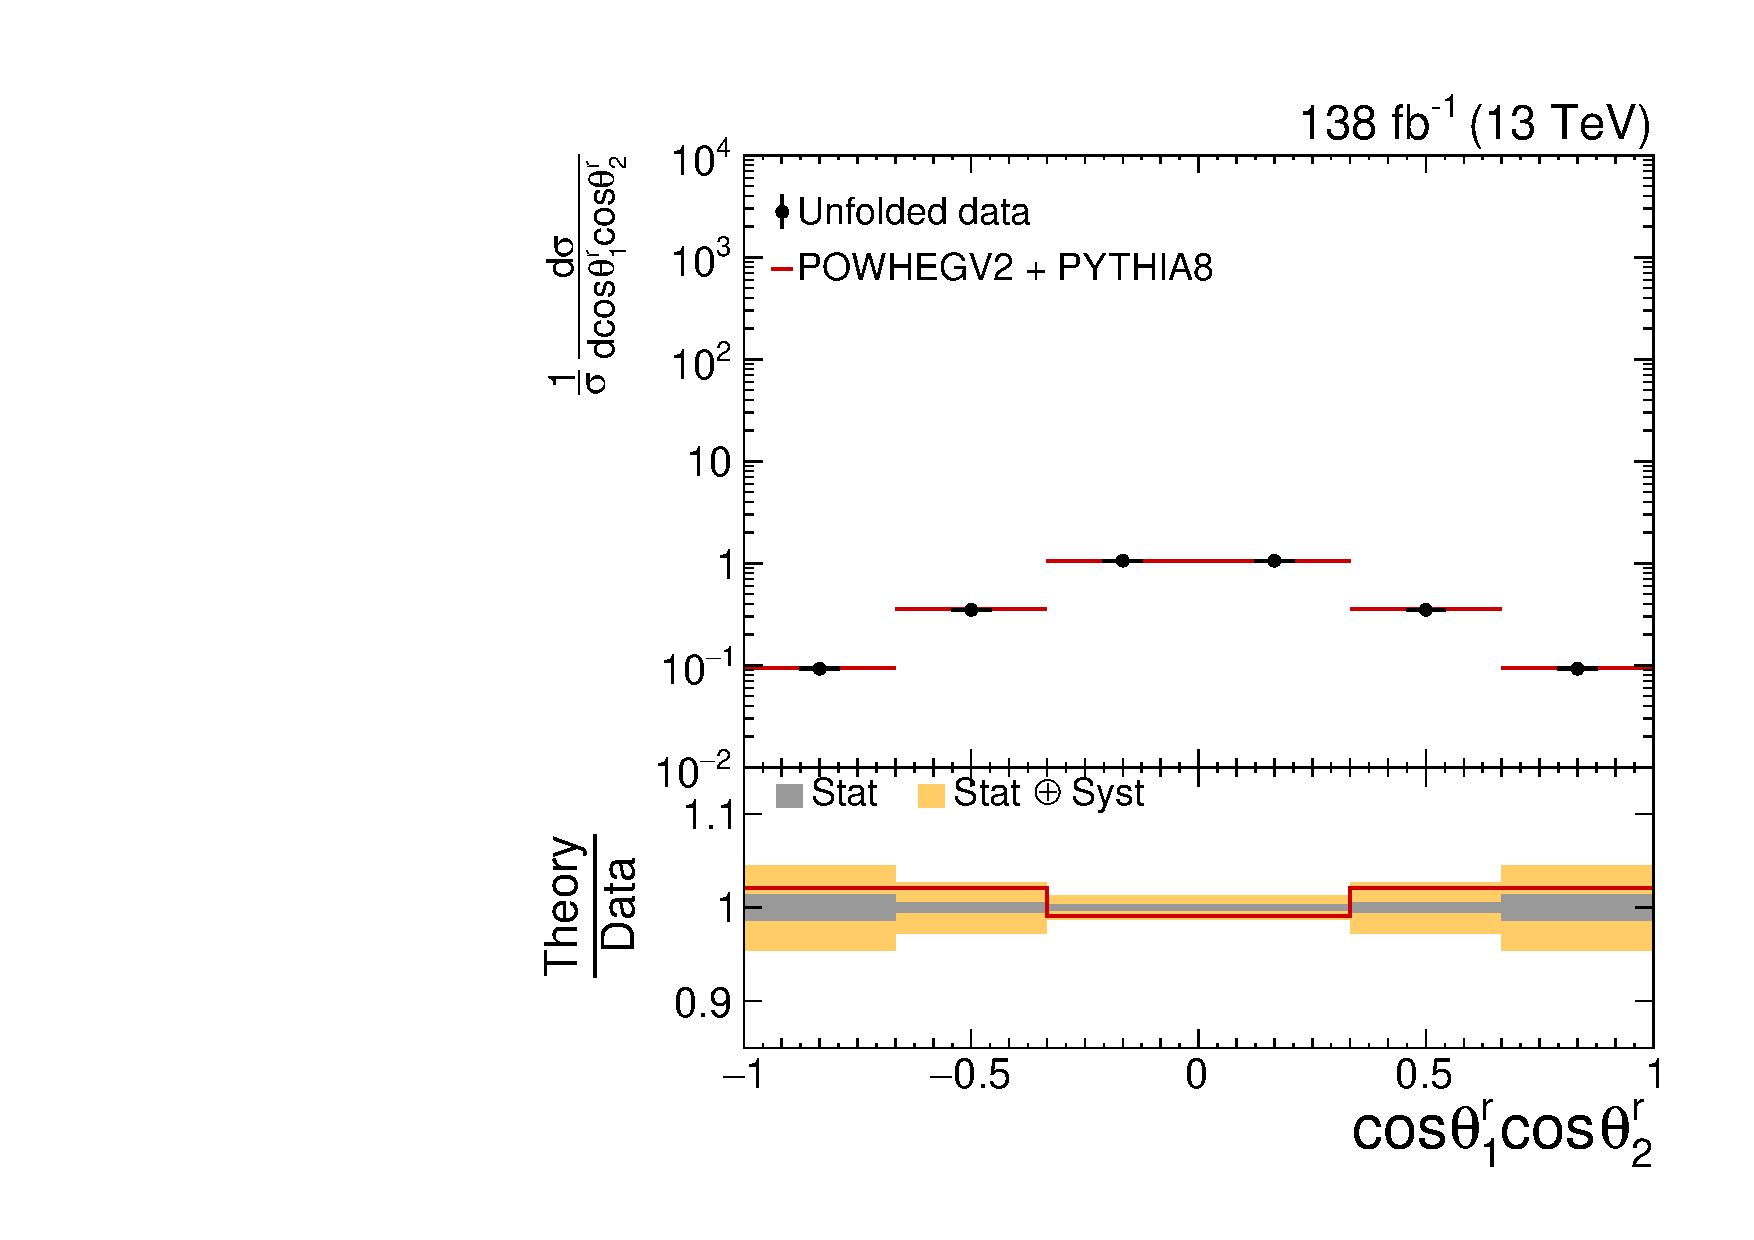
\includegraphics[width=0.40\textwidth]{fig_fullRun2UL/unfolding/combined/UnfoldedResultsNorm_c_rr.pdf} \\
\label{fig:c_rr}
\caption{Reconstructed detector-level distribution (Top Left), detector response-matrix (Top Right), absolute cross-section unfolded to parton-level (Bottom Left), and normalized cross-section unfolded to parton-level (Bottom Right) for diagonal spin correlation observable $\cos\theta_{1}^{r}\cos\theta_{2}^{r}$, from which spin-density coefficient $C_{rr}$ (sensitive to spin-density coefficient function $c_{r r}$) is extracted.}
\end{center}
\end{figure}
\clearpage
\begin{figure}[htb]
\begin{center}
 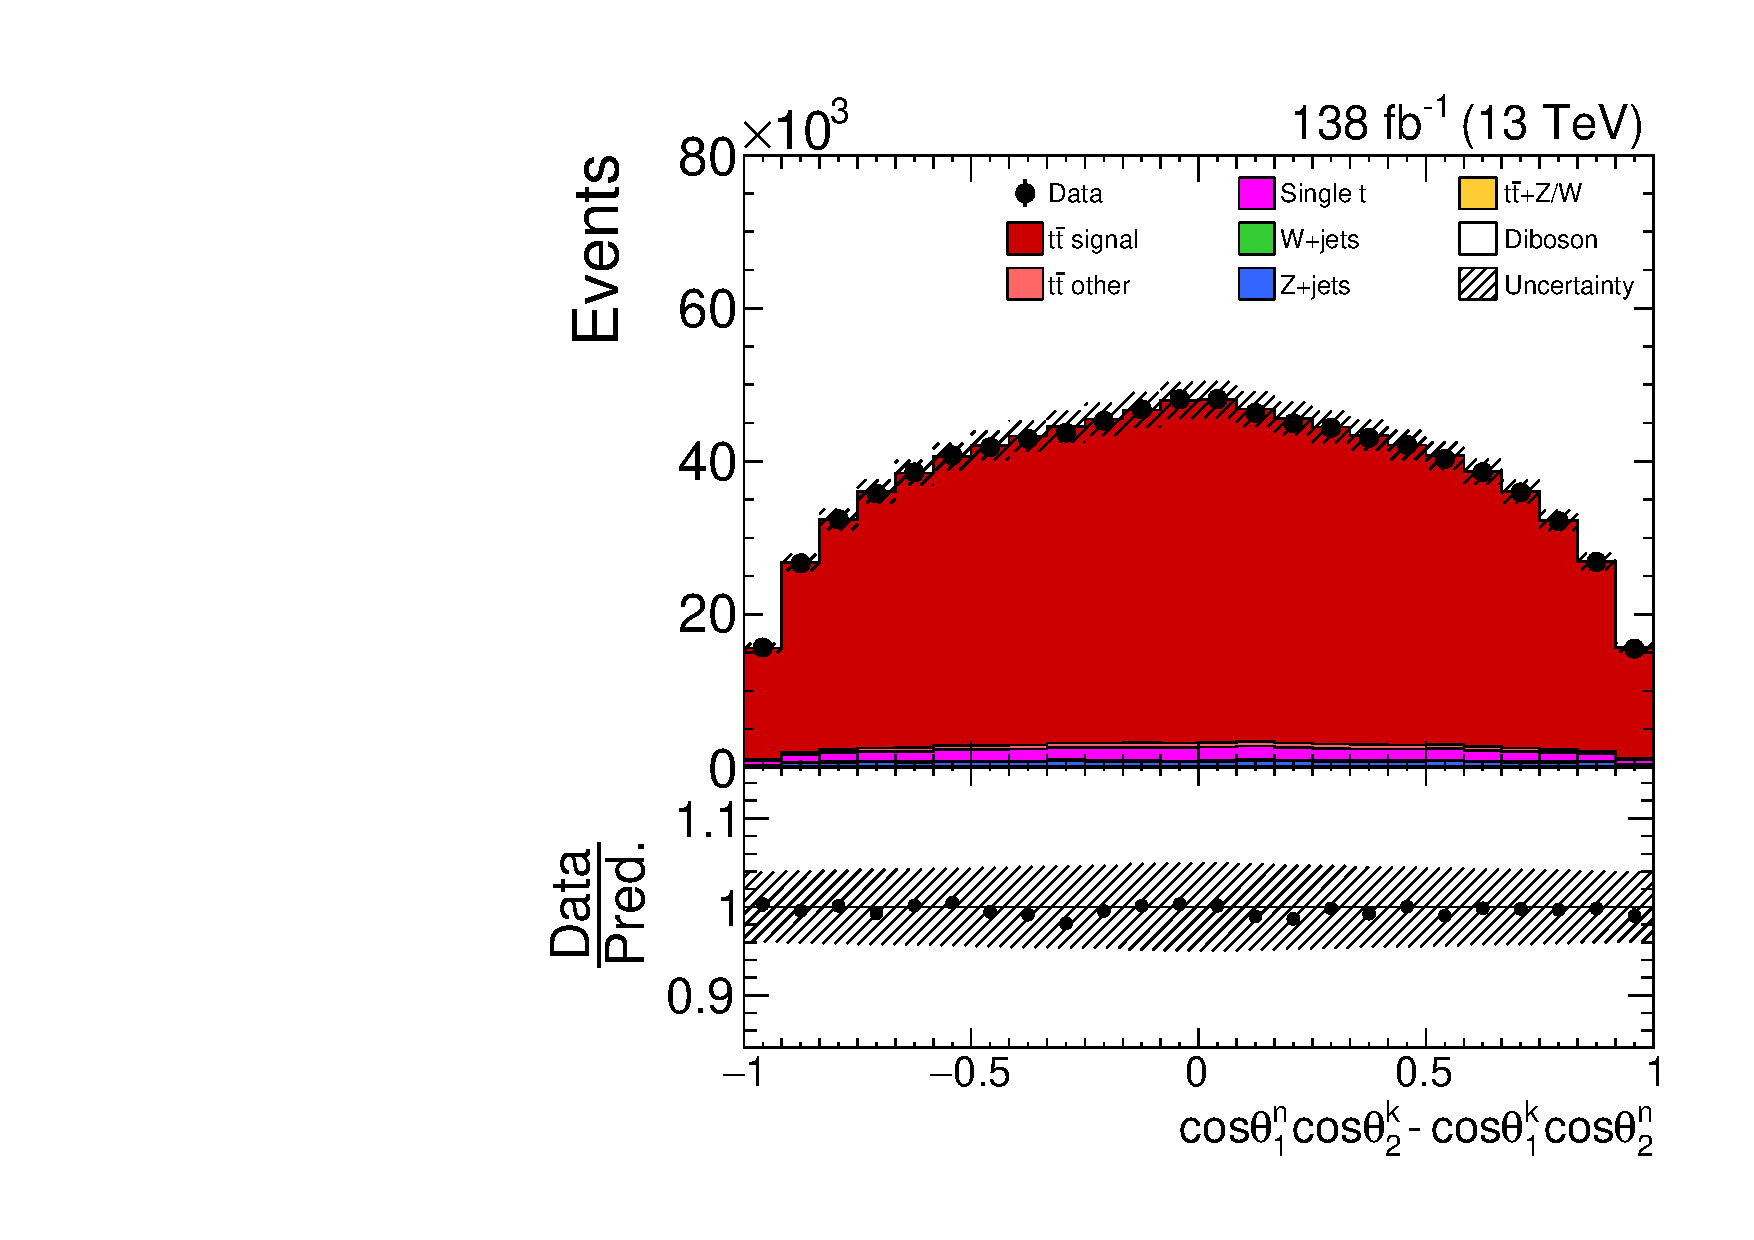
\includegraphics[width=0.40\textwidth]{fig_fullRun2UL/controlplots/combined/Hyp_LLBarCMnk.pdf}
 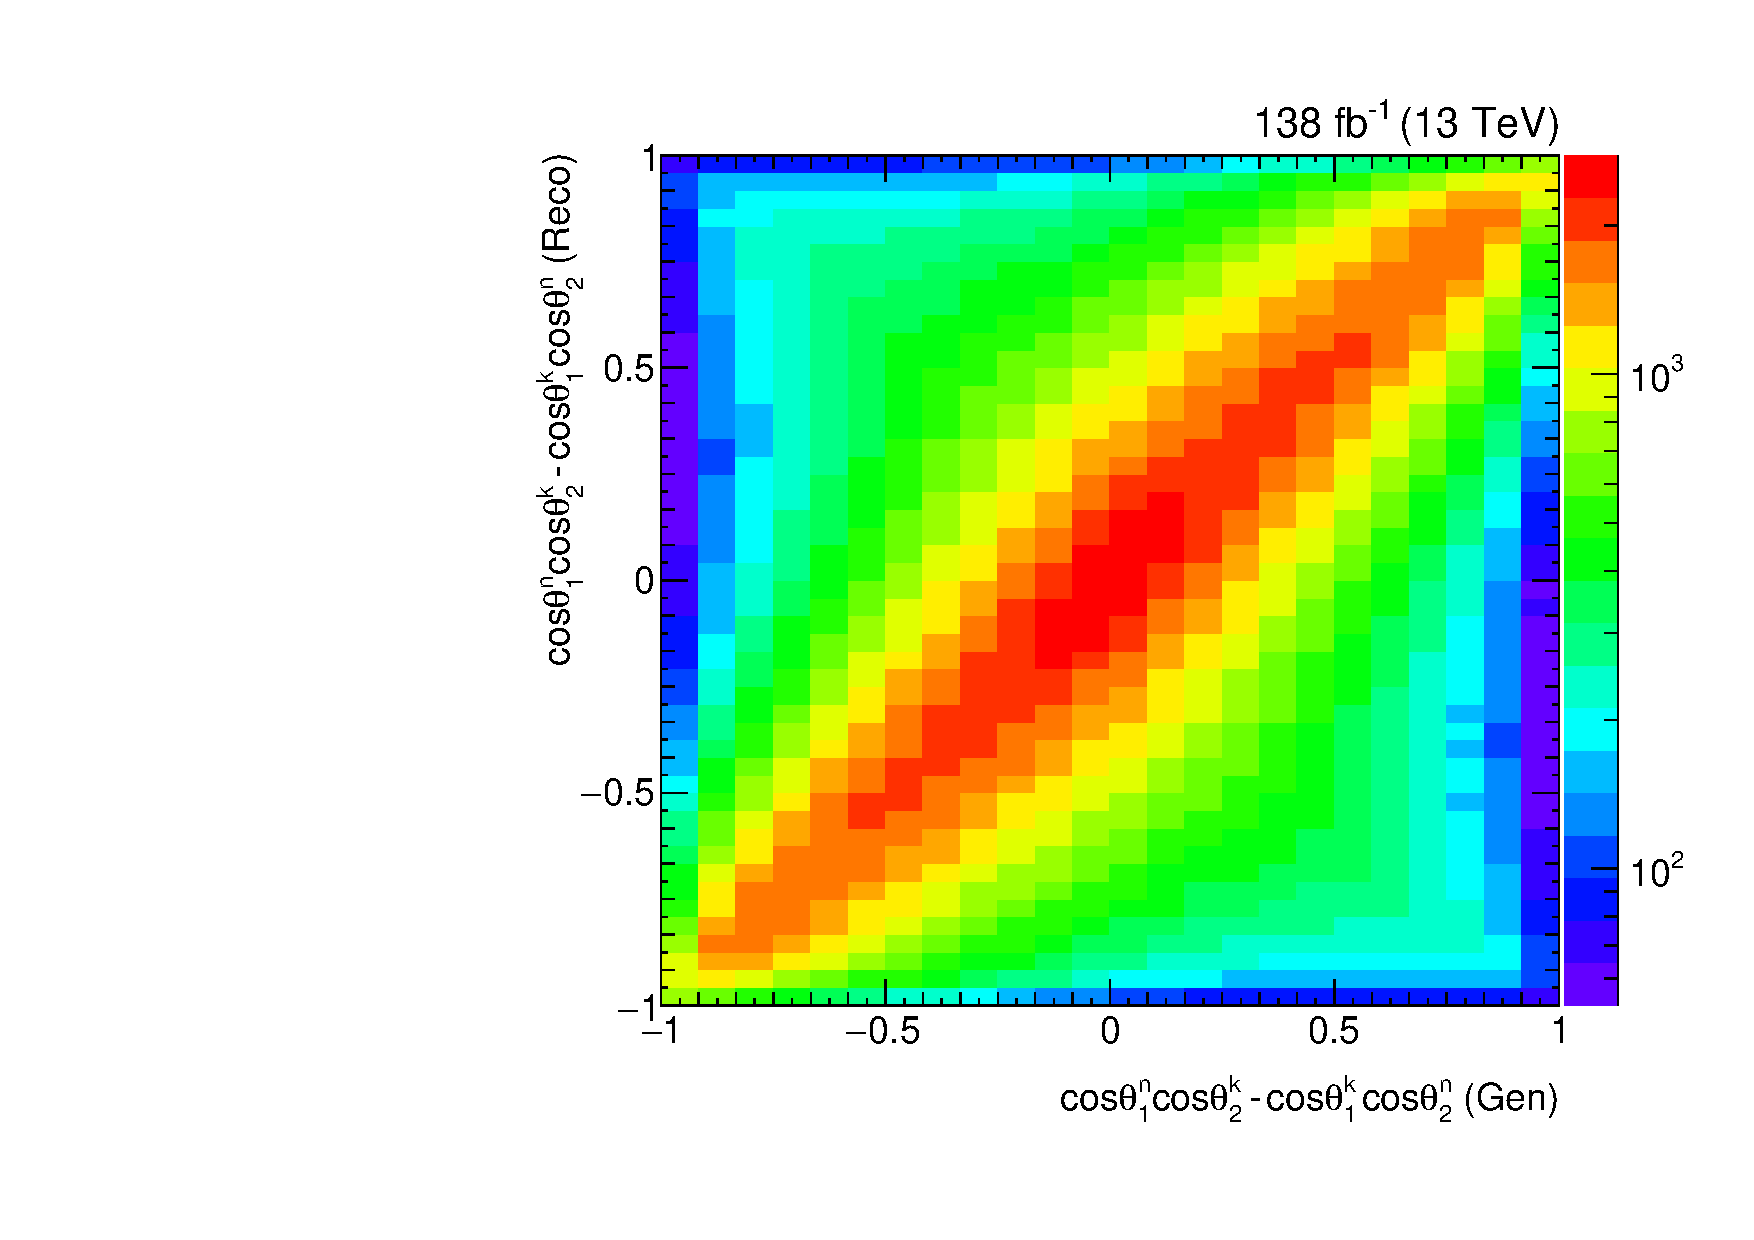
\includegraphics[width=0.40\textwidth]{fig_fullRun2UL/unfolding/combined/ResponseMatrix_c_Mnk.pdf} \\
 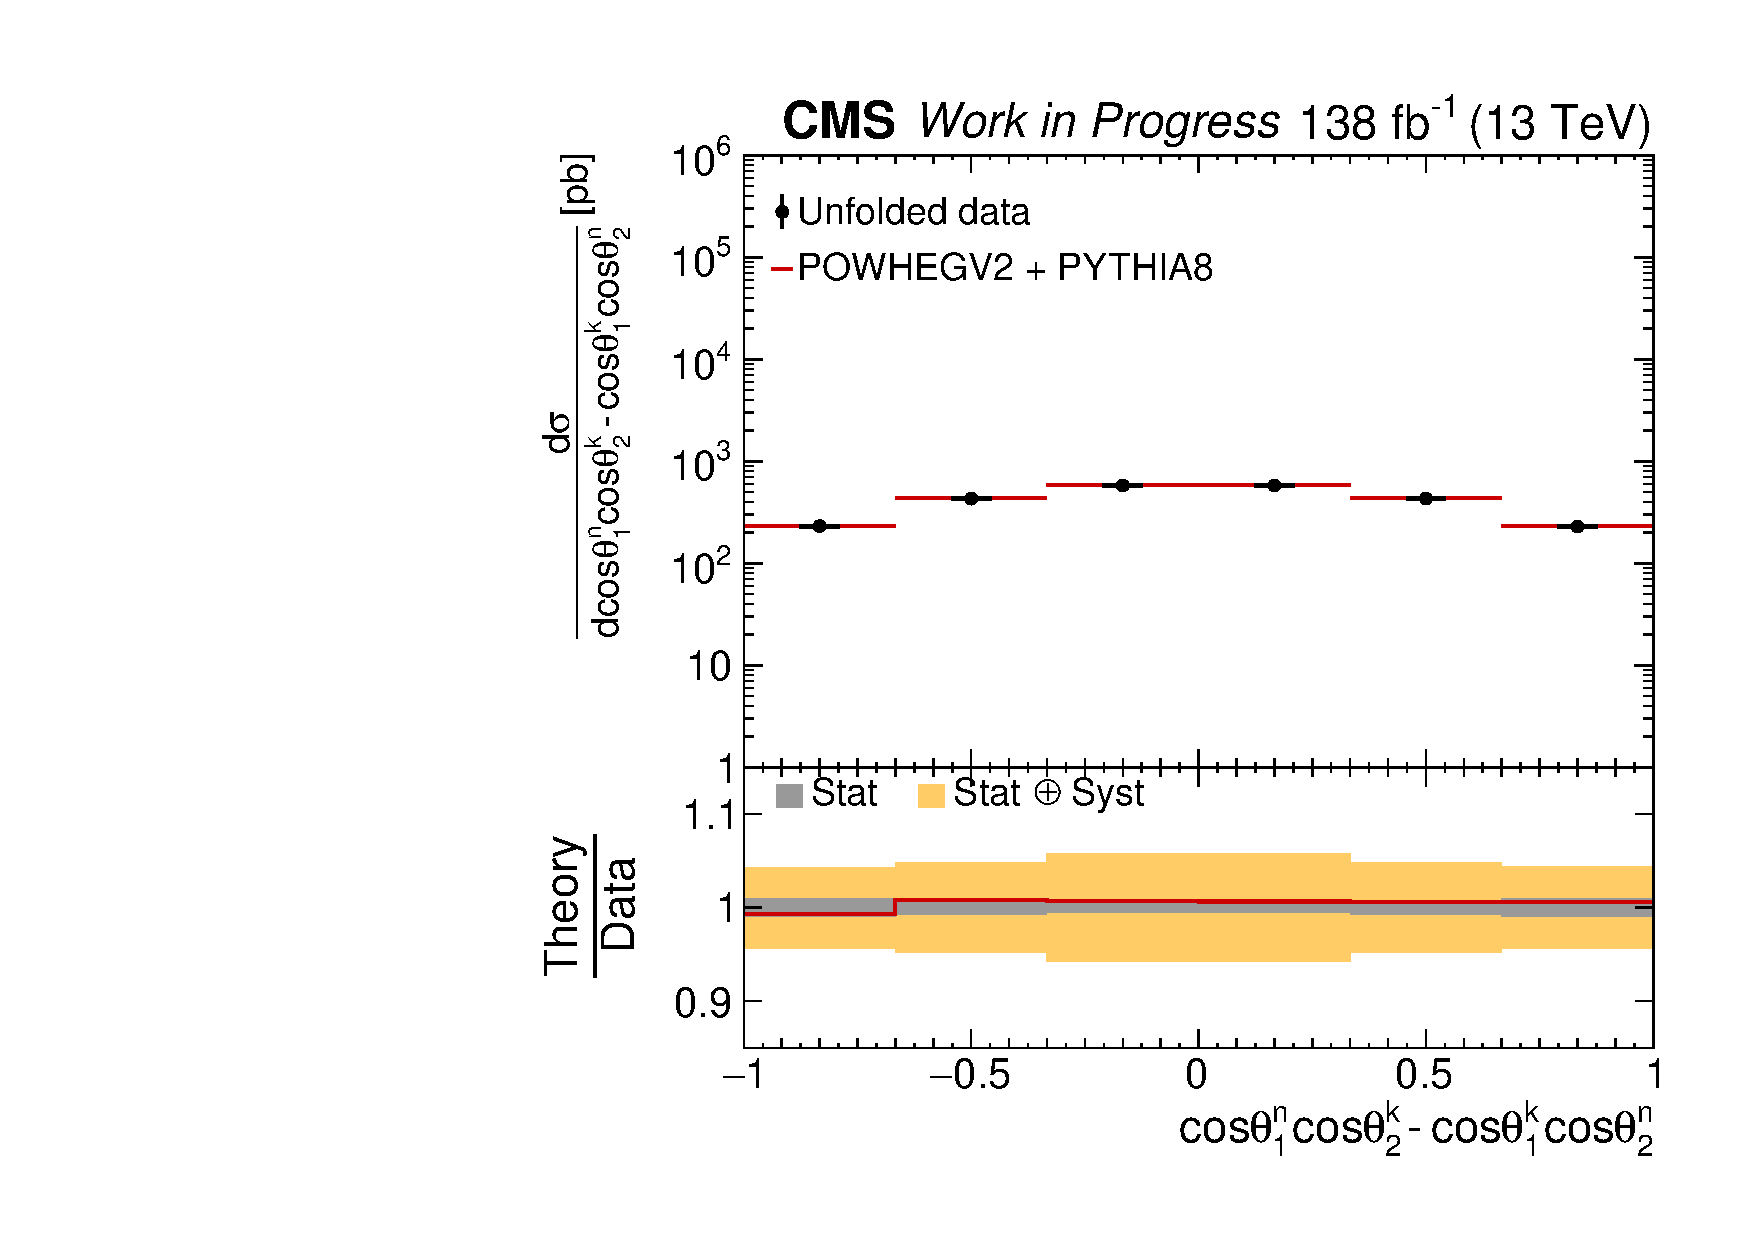
\includegraphics[width=0.40\textwidth]{fig_fullRun2UL/unfolding/combined/UnfoldedResults_c_Mnk.pdf}
 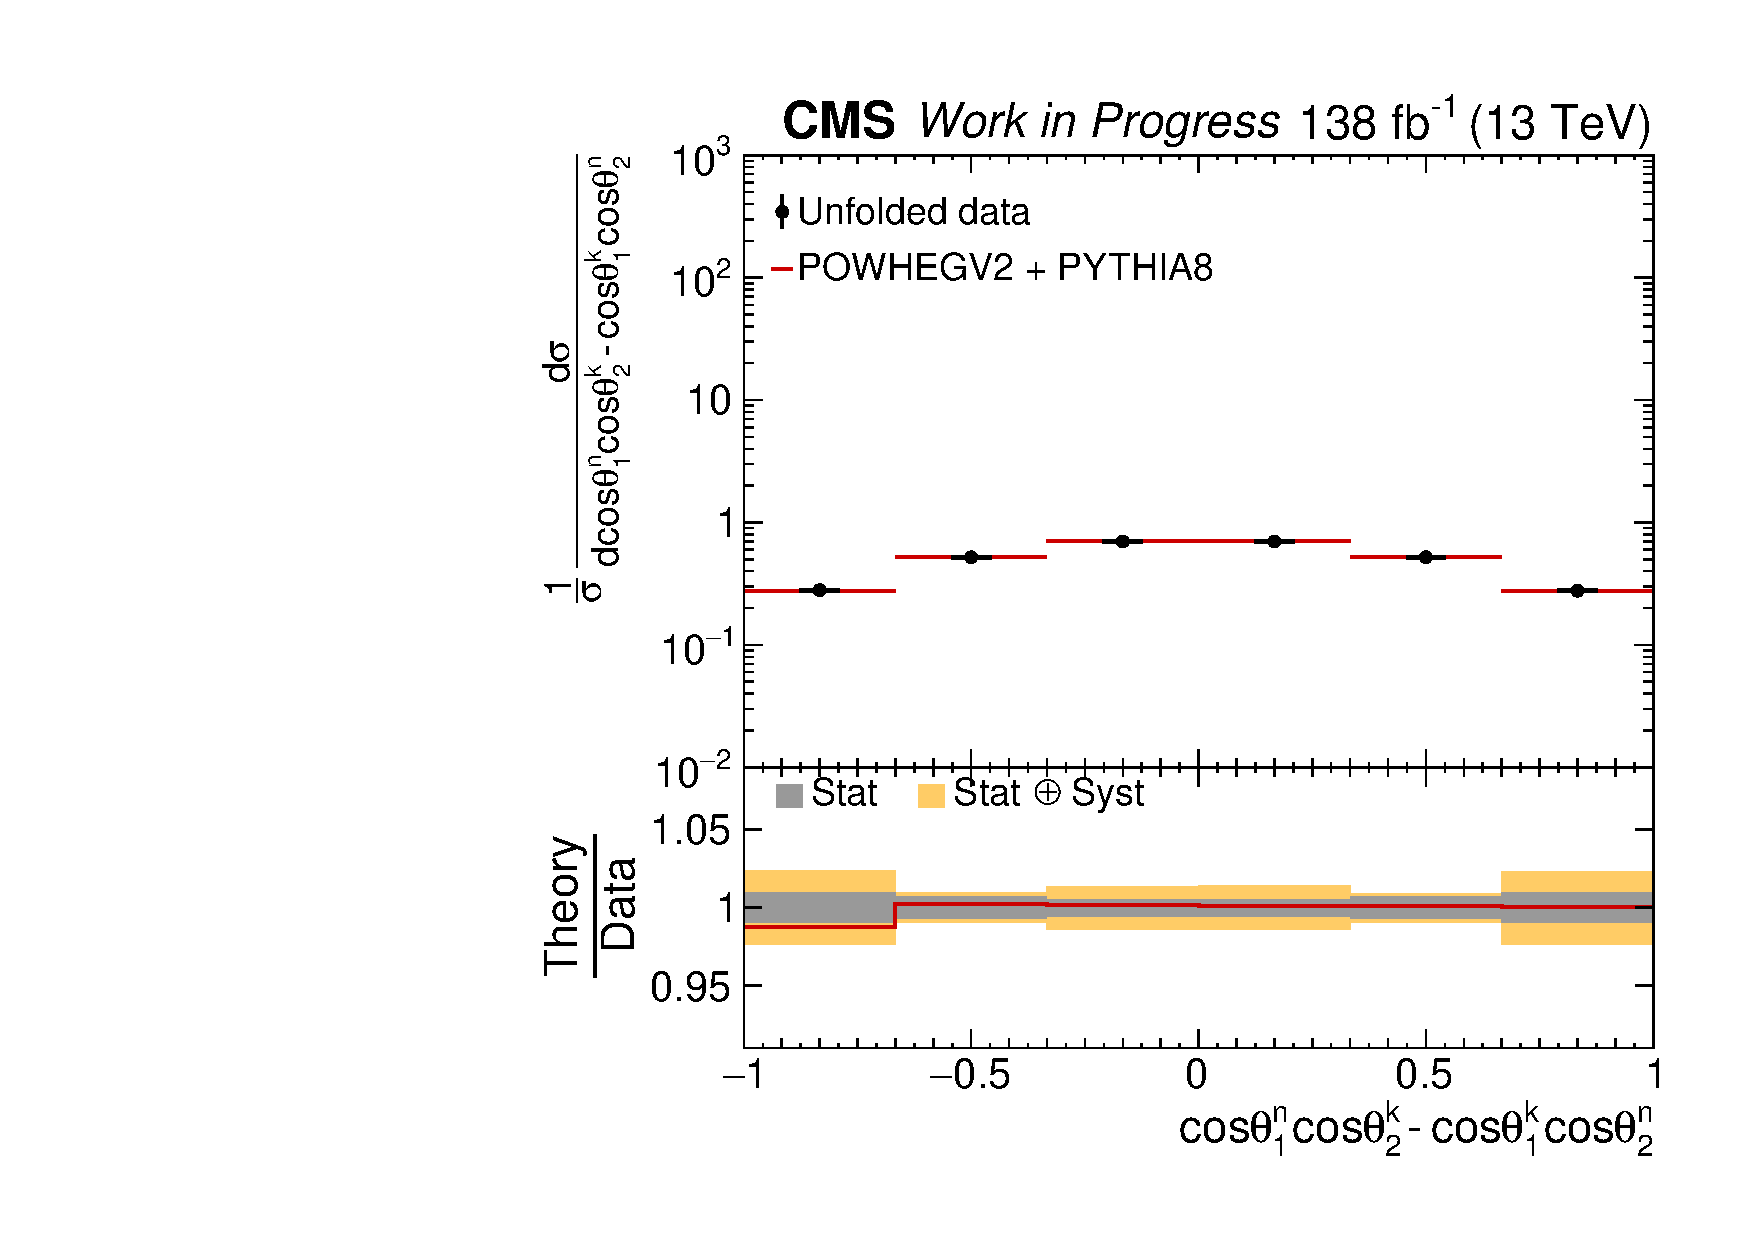
\includegraphics[width=0.40\textwidth]{fig_fullRun2UL/unfolding/combined/UnfoldedResultsNorm_c_Mnk.pdf} \\
\label{fig:c_Mnk}
\caption{Reconstructed detector-level distribution (Top Left), detector response-matrix (Top Right), absolute cross-section unfolded to parton-level (Bottom Left), and normalized cross-section unfolded to parton-level (Bottom Right) for off-diagonal spin correlation difference observable $\cos\theta_{1}^{n}\cos\theta_{2}^{k}-\cos\theta_{1}^{k}\cos\theta_{2}^{n}$, from which spin-density coefficient $C_{nk}-C_{kn}$ (sensitive to spin-density coefficient function $-c_r$) is extracted.}
\end{center}
\end{figure}
\clearpage
\begin{figure}[htb]
\begin{center}
 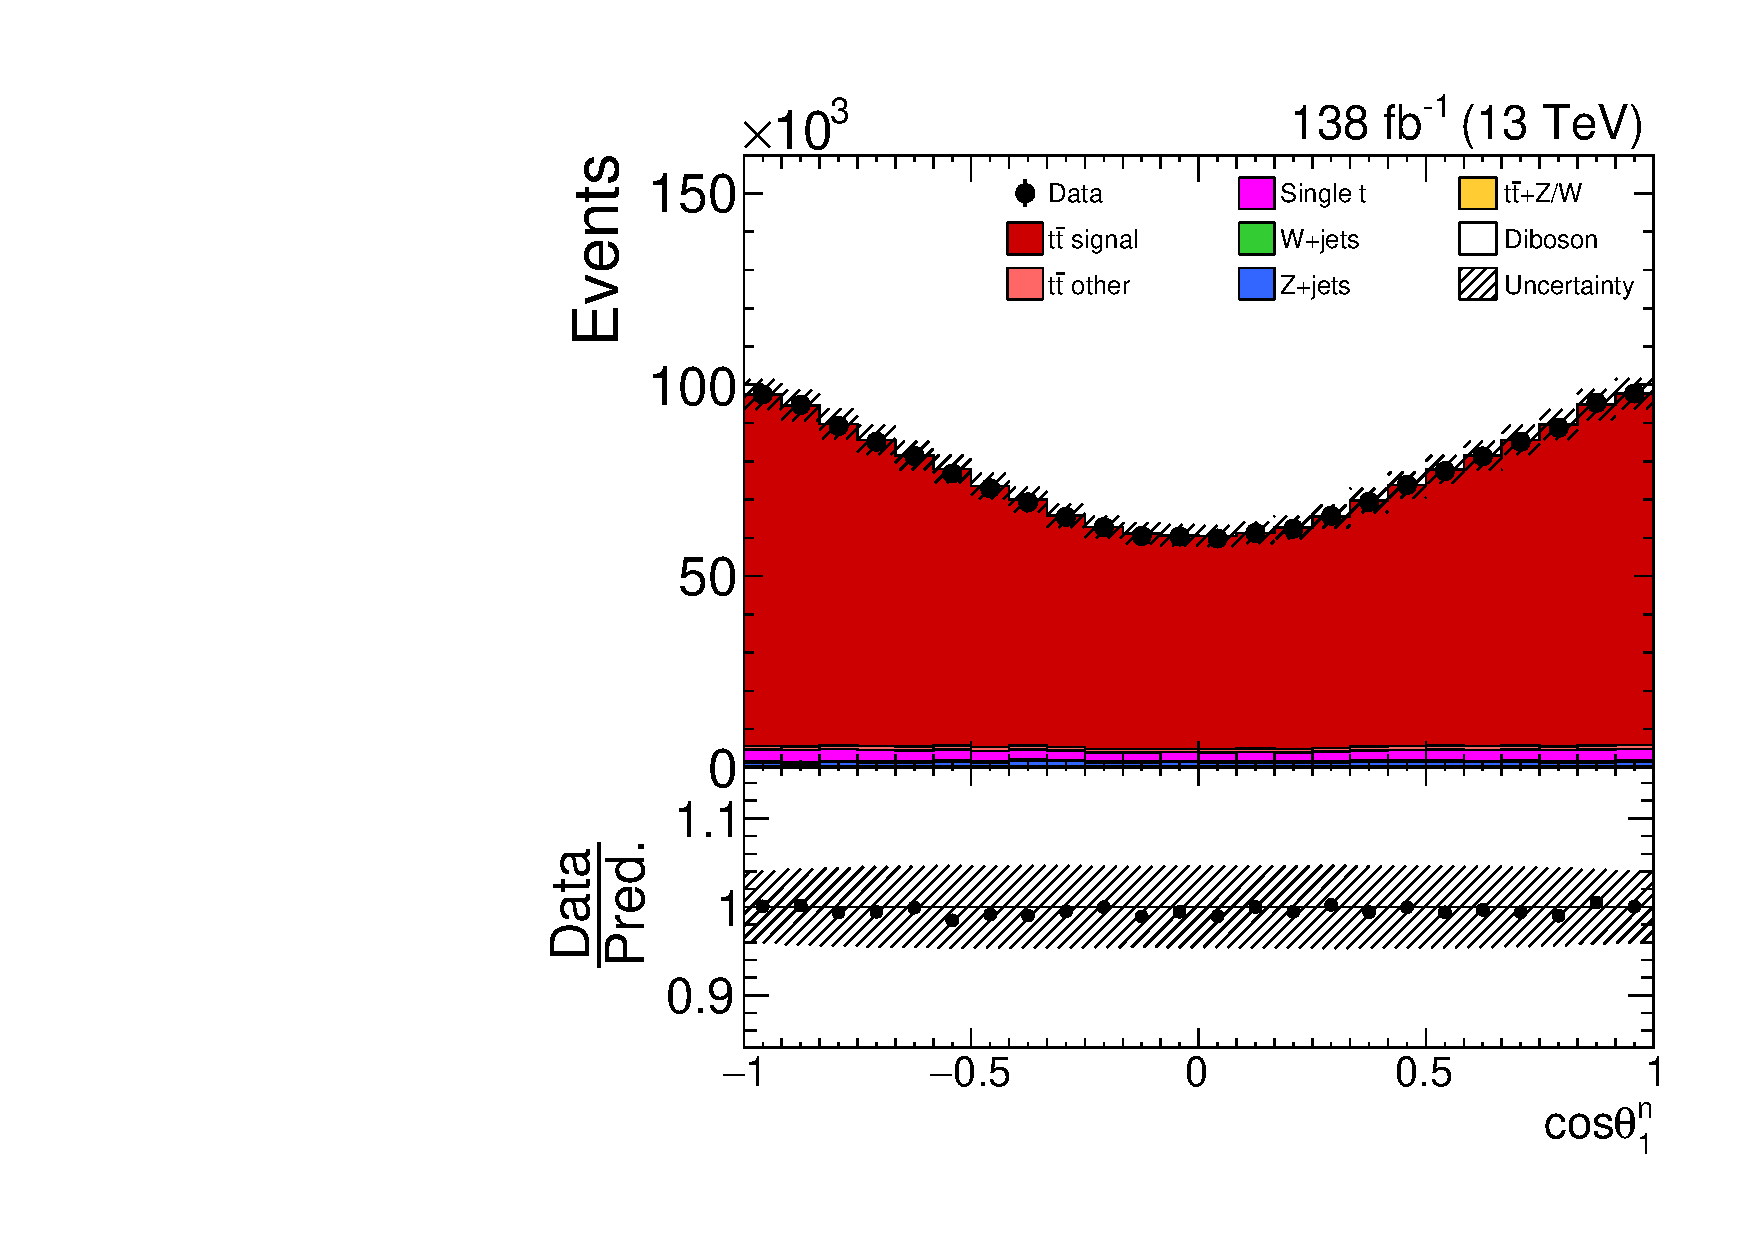
\includegraphics[width=0.40\textwidth]{fig_fullRun2UL/controlplots/combined/Hyp_AntiLeptonBn.pdf}
 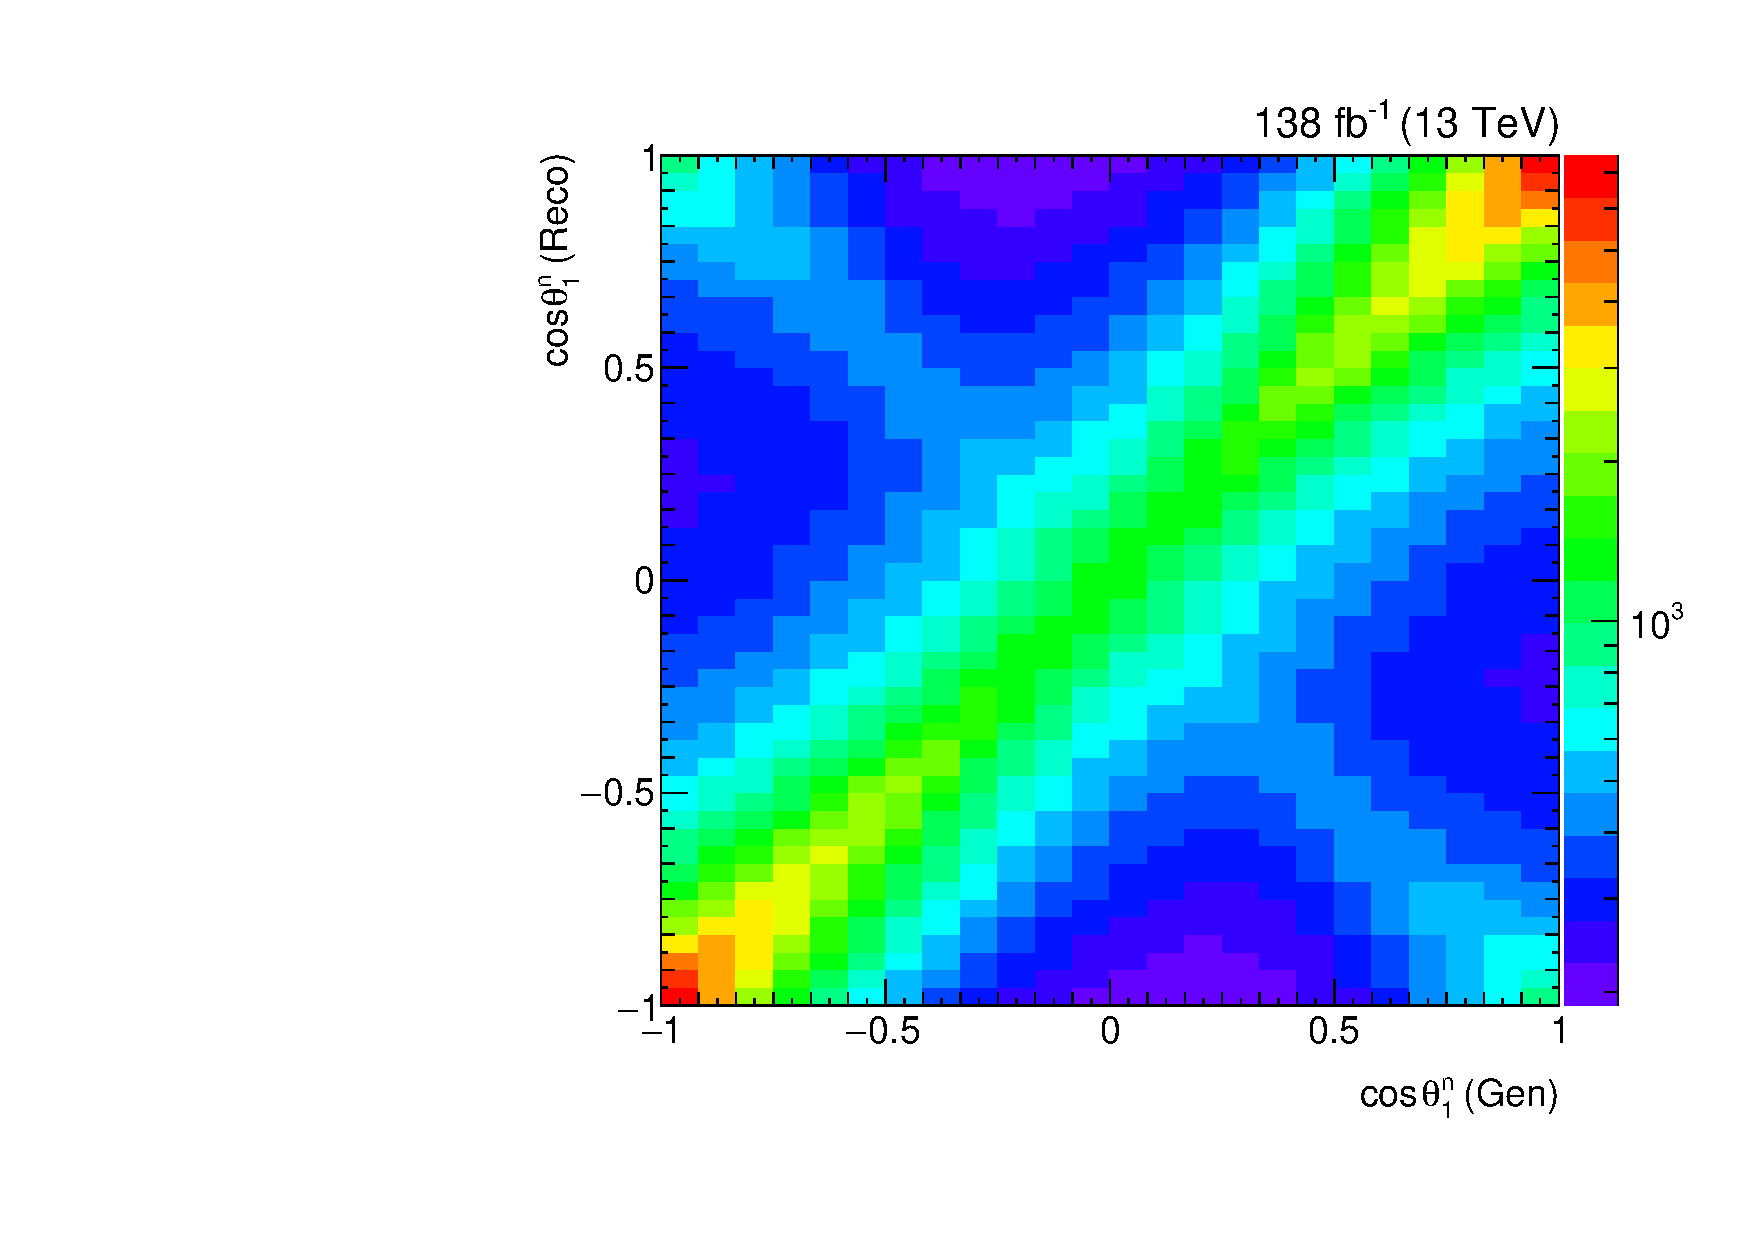
\includegraphics[width=0.40\textwidth]{fig_fullRun2UL/unfolding/combined/ResponseMatrix_b1n.pdf} \\
 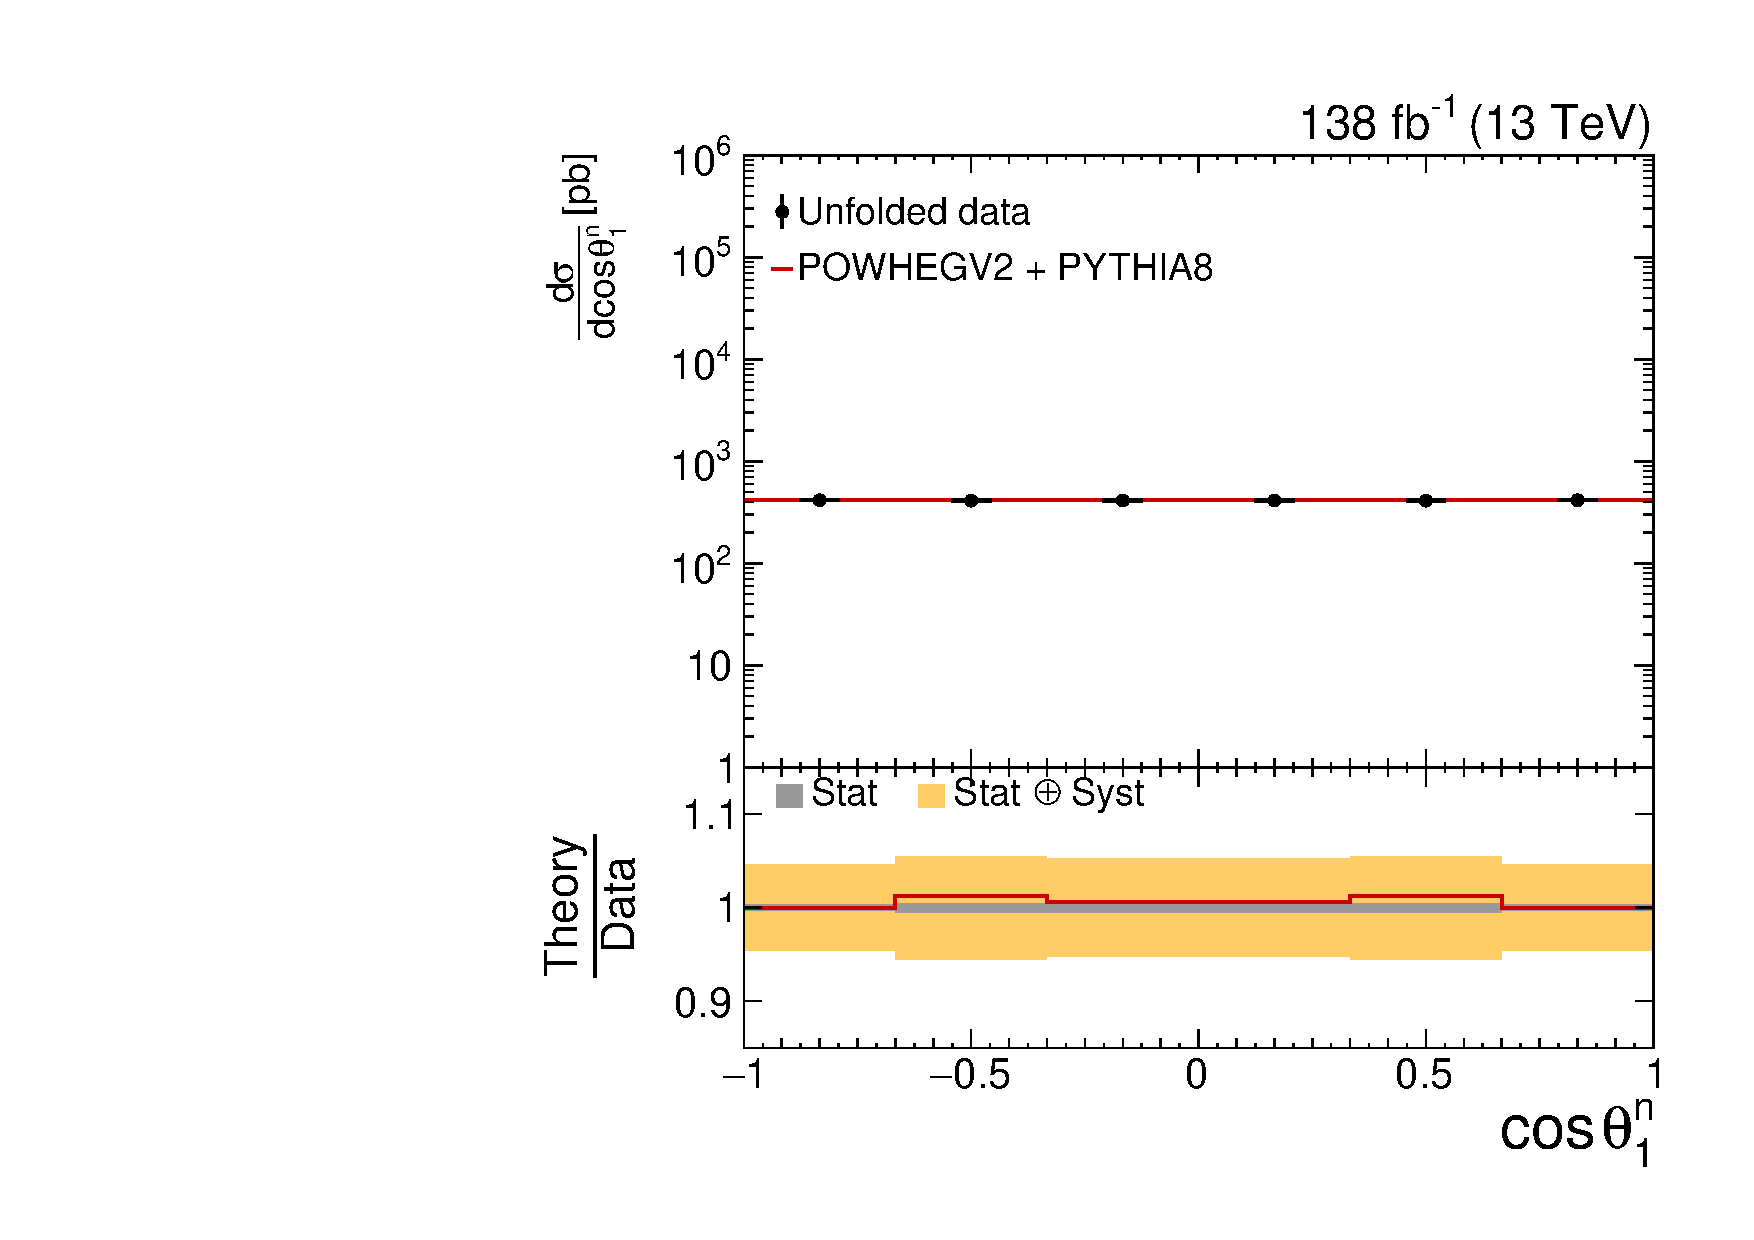
\includegraphics[width=0.40\textwidth]{fig_fullRun2UL/unfolding/combined/UnfoldedResults_b1n.pdf}
 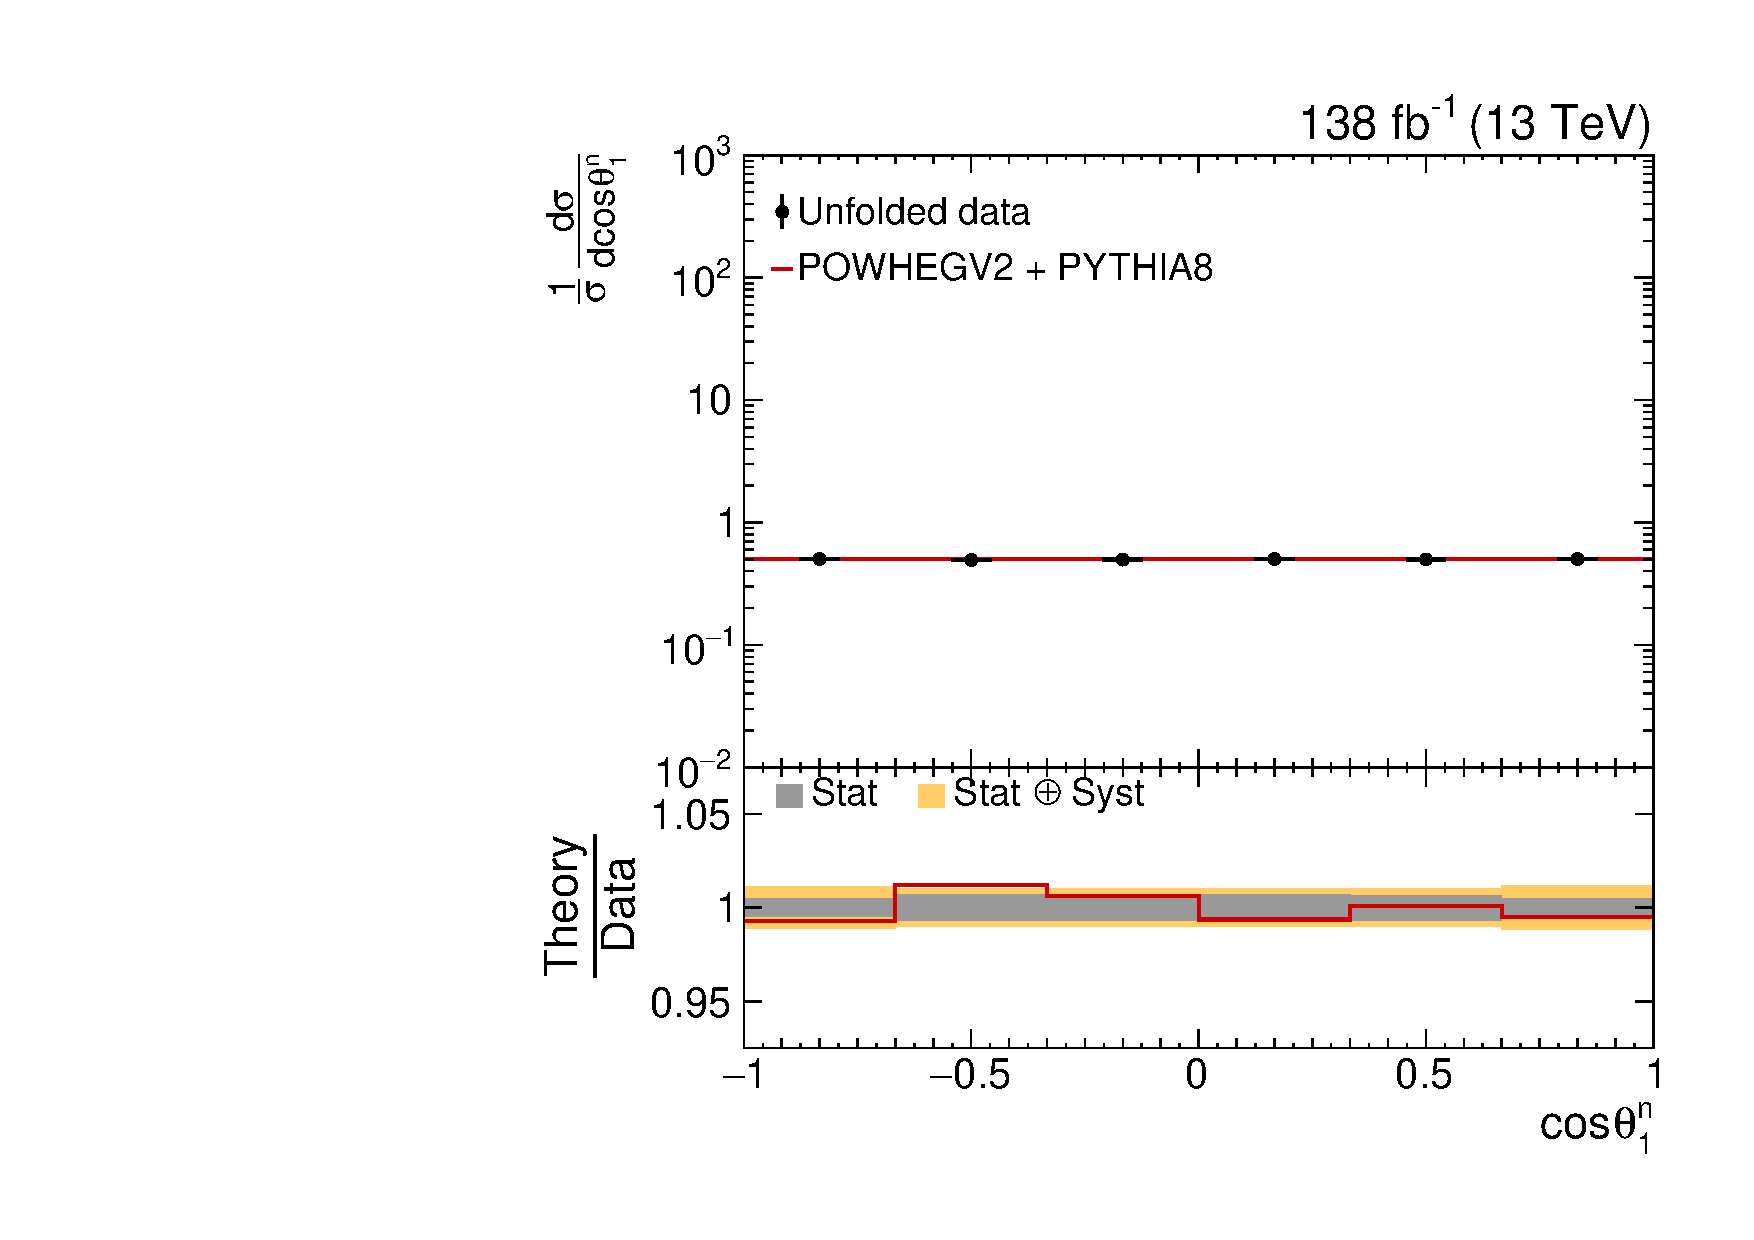
\includegraphics[width=0.40\textwidth]{fig_fullRun2UL/unfolding/combined/UnfoldedResultsNorm_b1n.pdf} \\
\label{fig:b1n}
\caption{Reconstructed detector-level distribution (Top Left), detector response-matrix (Top Right), absolute cross-section unfolded to parton-level (Bottom Left), and normalized cross-section unfolded to parton-level (Bottom Right) for polarization observable $\cos\theta_{1}^{n}$, from which spin-density coefficient $B_{1}^{n}$ (sensitive to spin-density coefficient function $b_n^{+}$) is extracted.}
\end{center}
\end{figure}
\clearpage
\begin{figure}[htb]
\begin{center}
 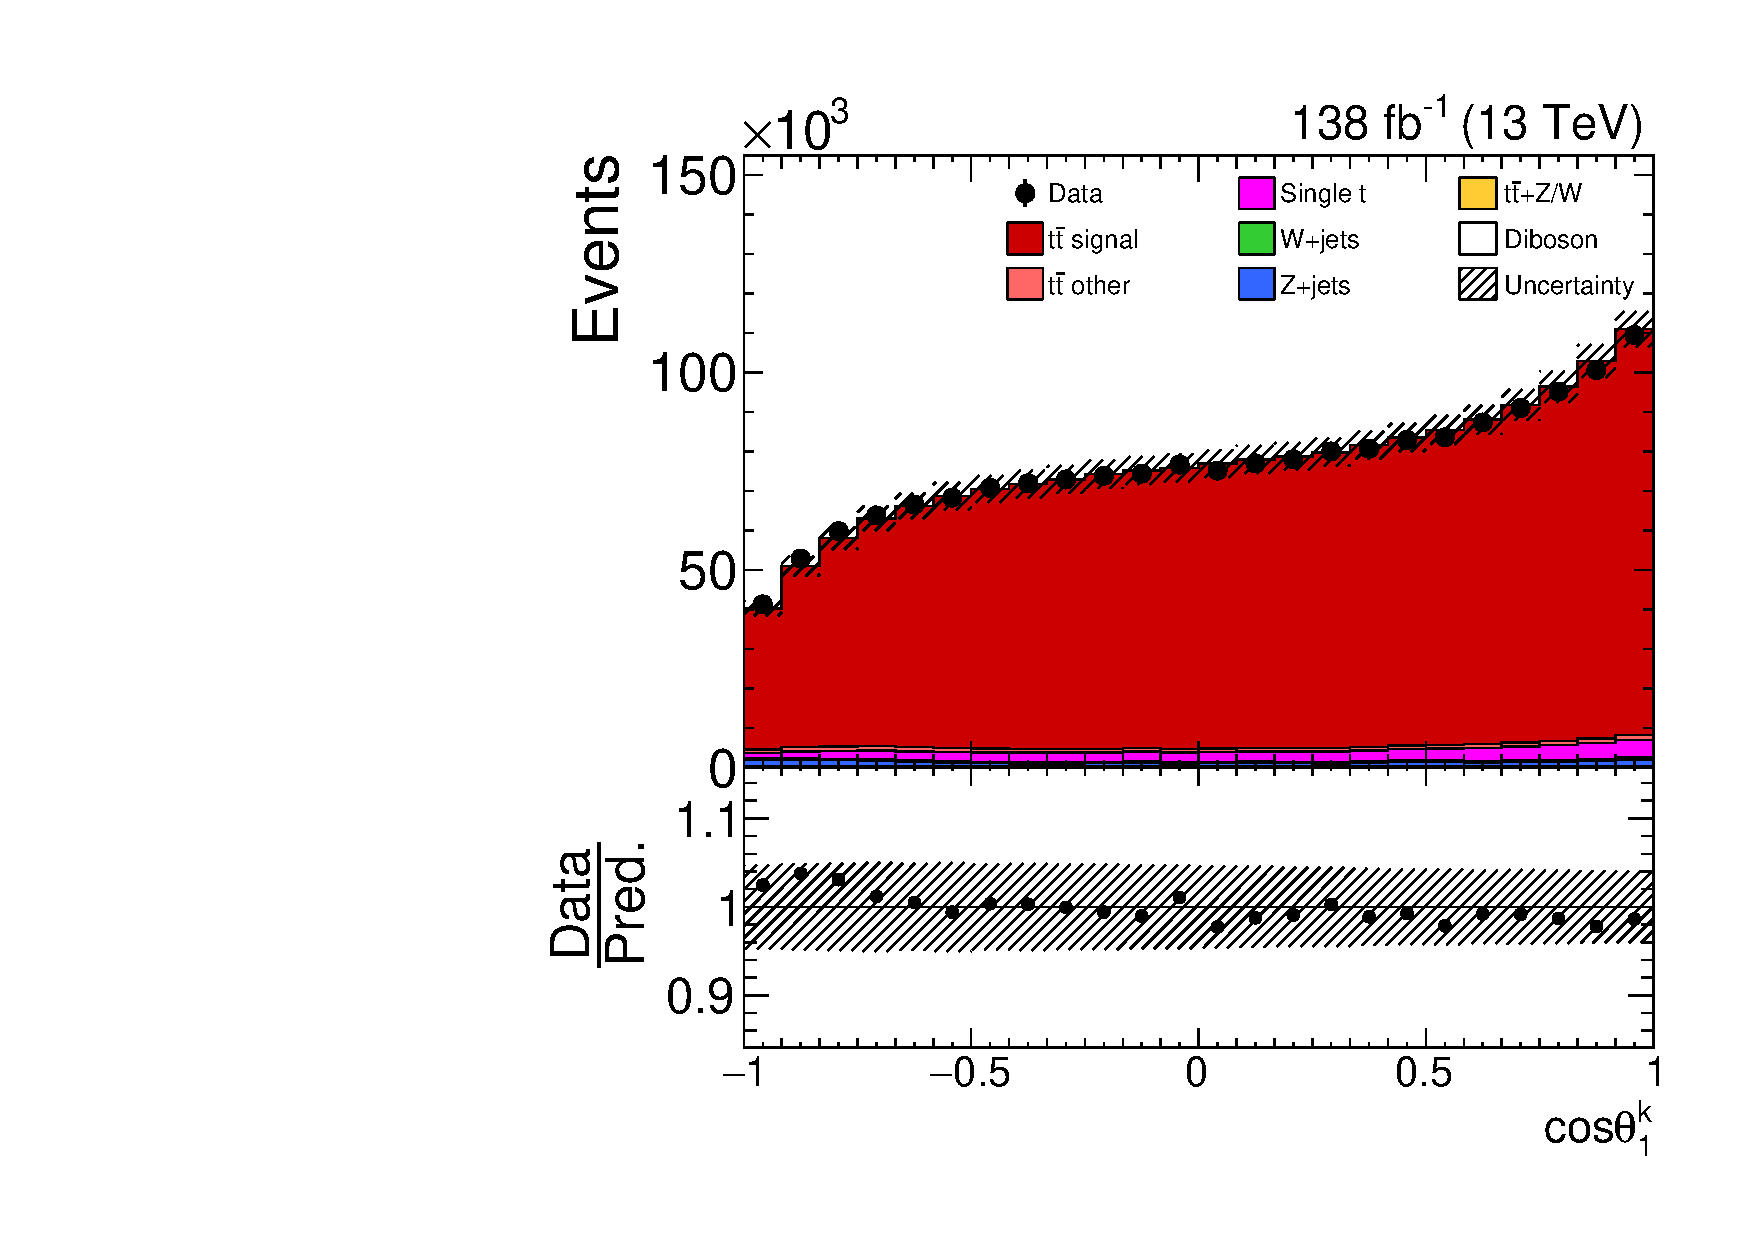
\includegraphics[width=0.40\textwidth]{fig_fullRun2UL/controlplots/combined/Hyp_AntiLeptonBk.pdf}
 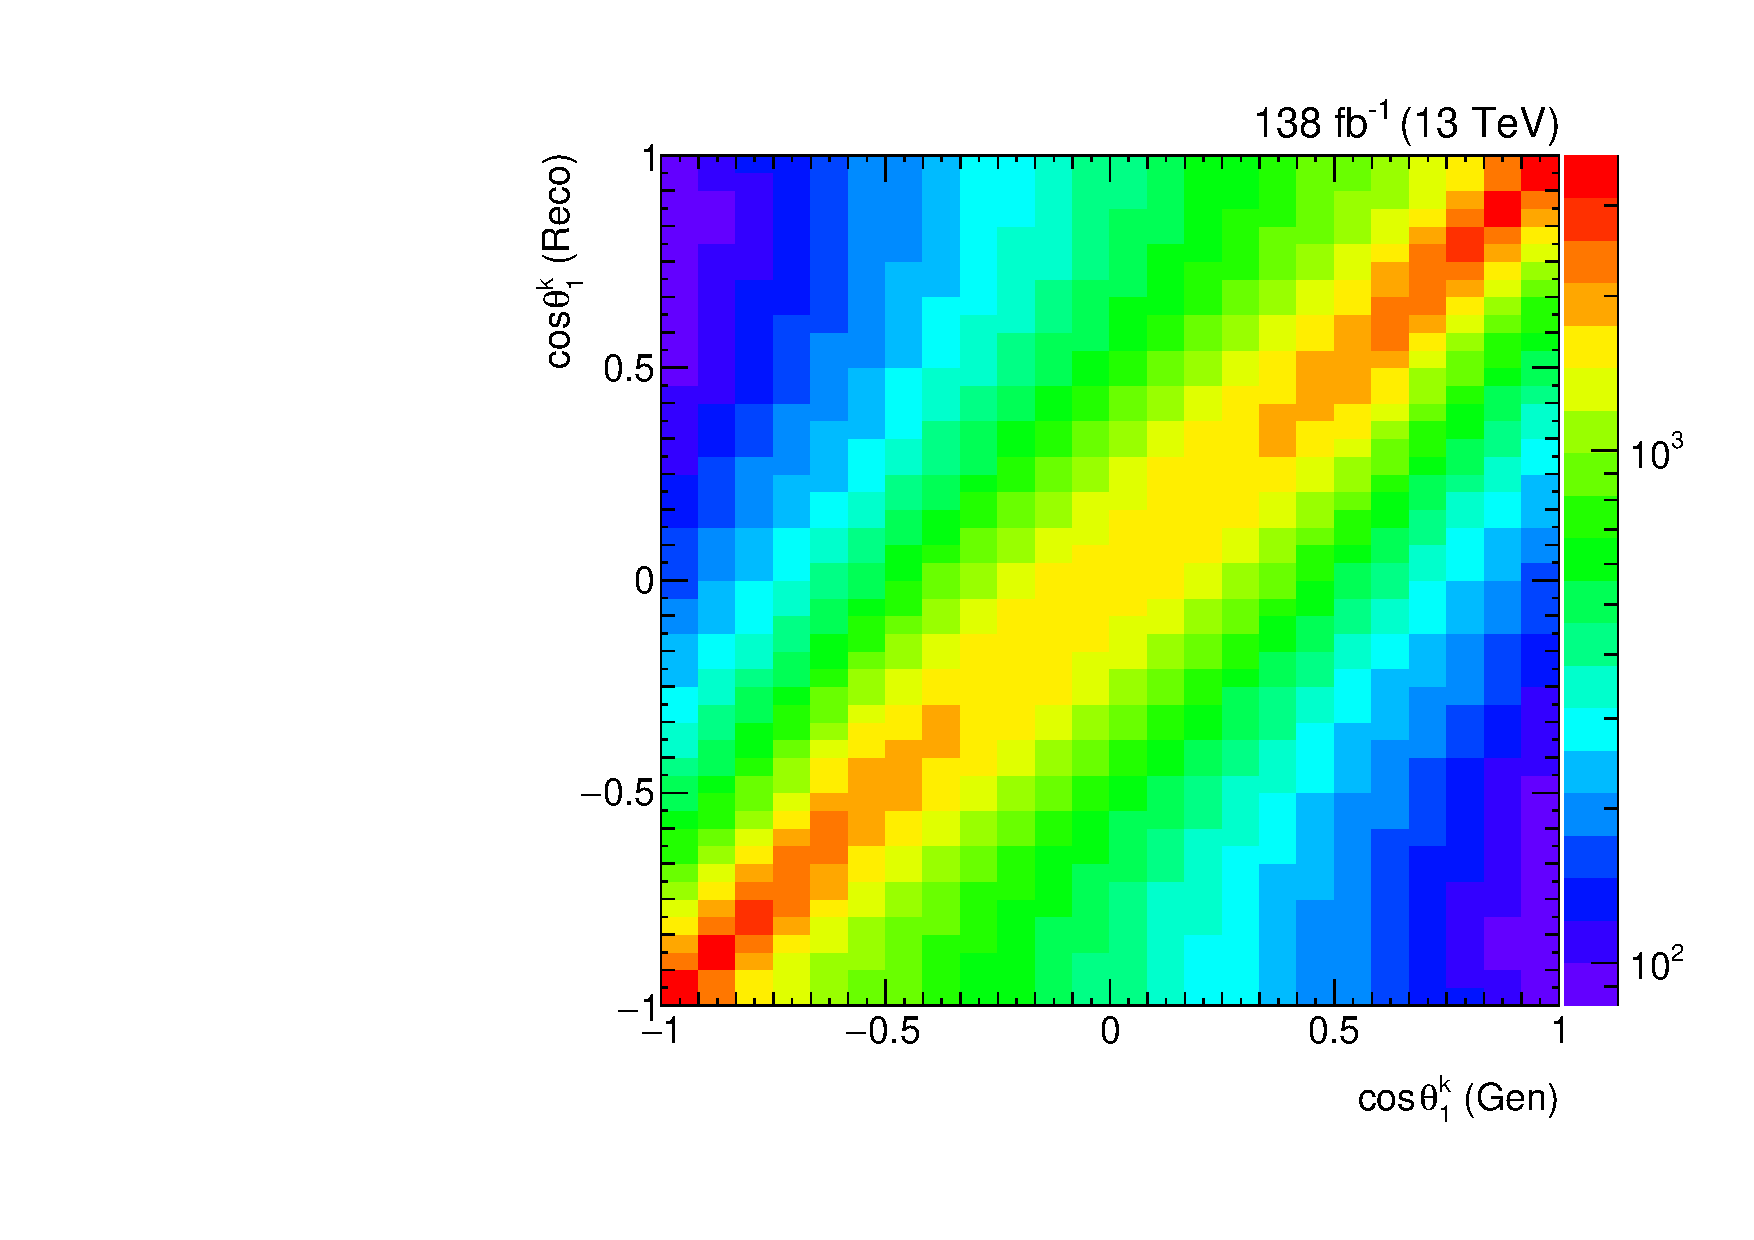
\includegraphics[width=0.40\textwidth]{fig_fullRun2UL/unfolding/combined/ResponseMatrix_b1k.pdf} \\
 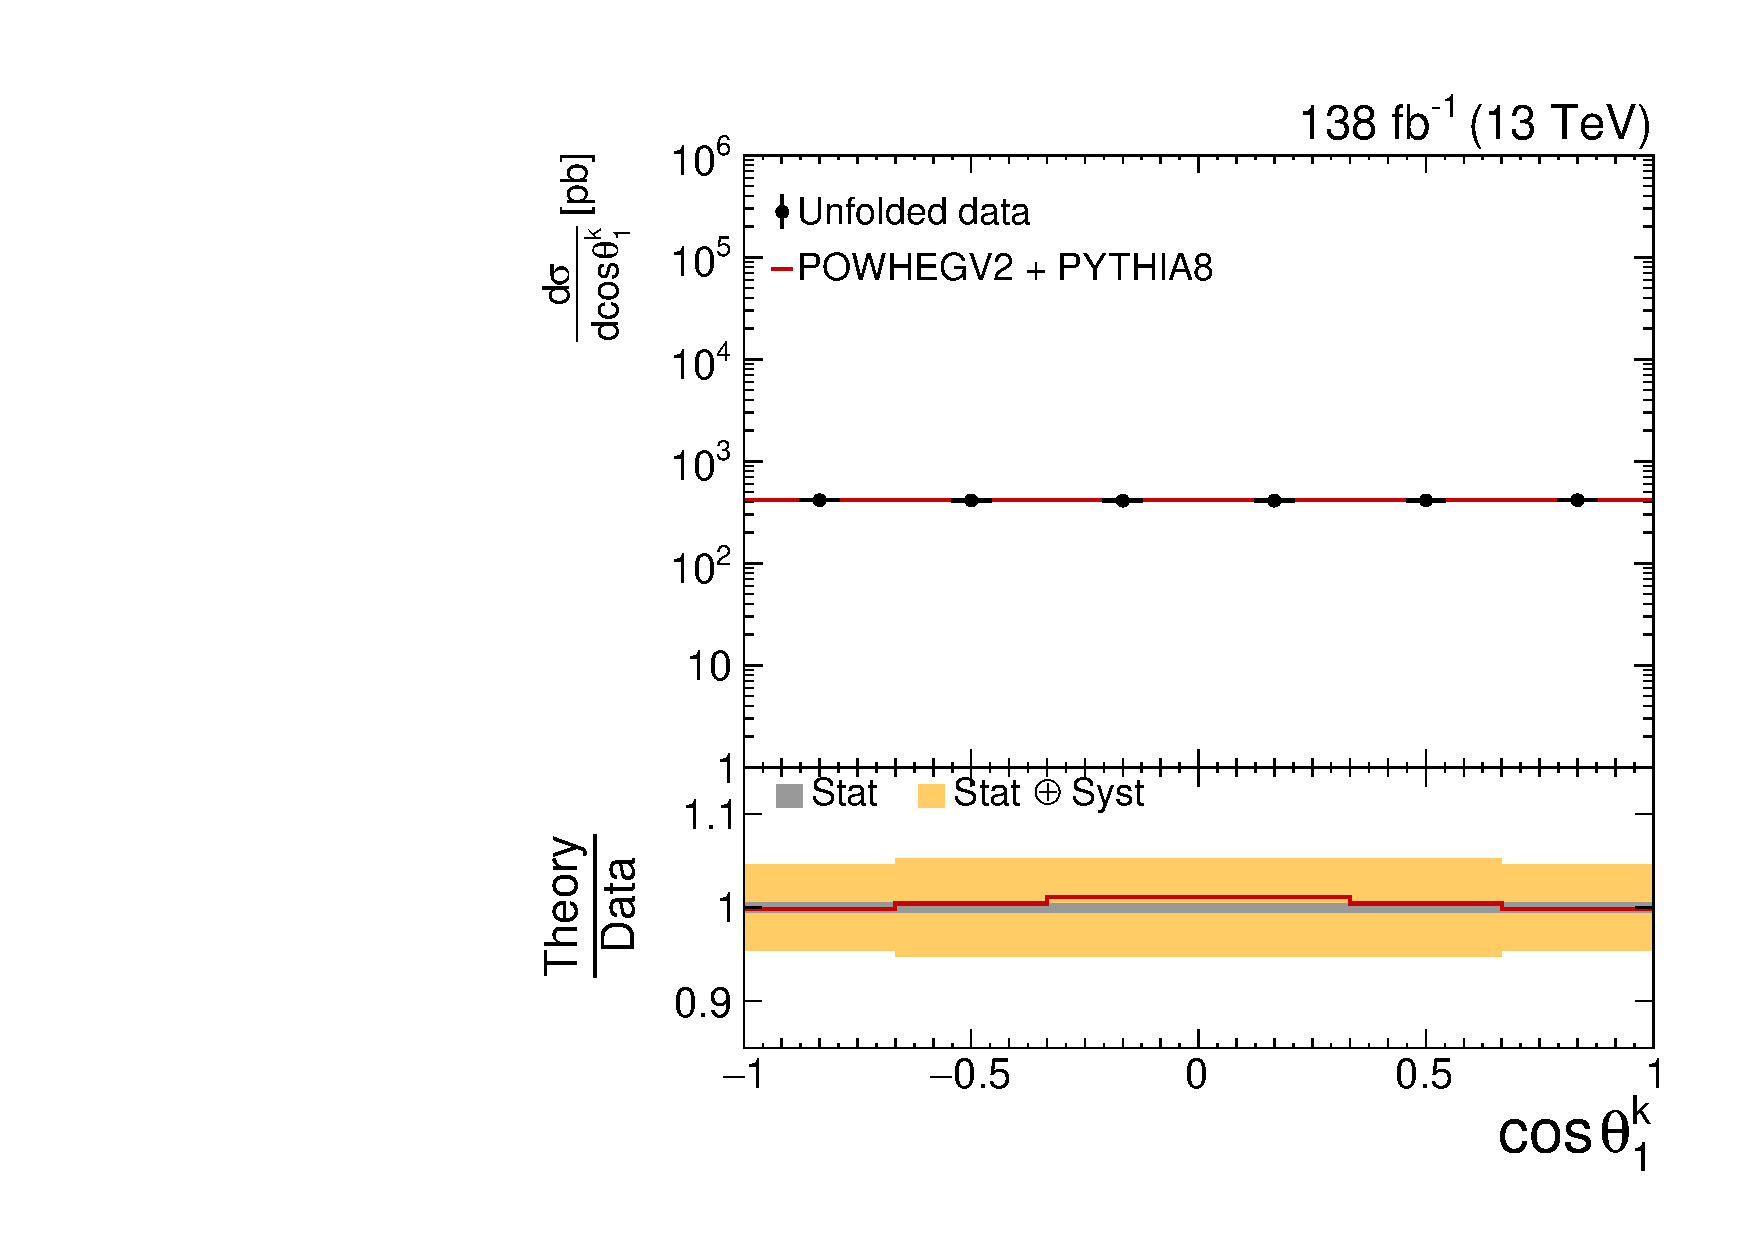
\includegraphics[width=0.40\textwidth]{fig_fullRun2UL/unfolding/combined/UnfoldedResults_b1k.pdf}
 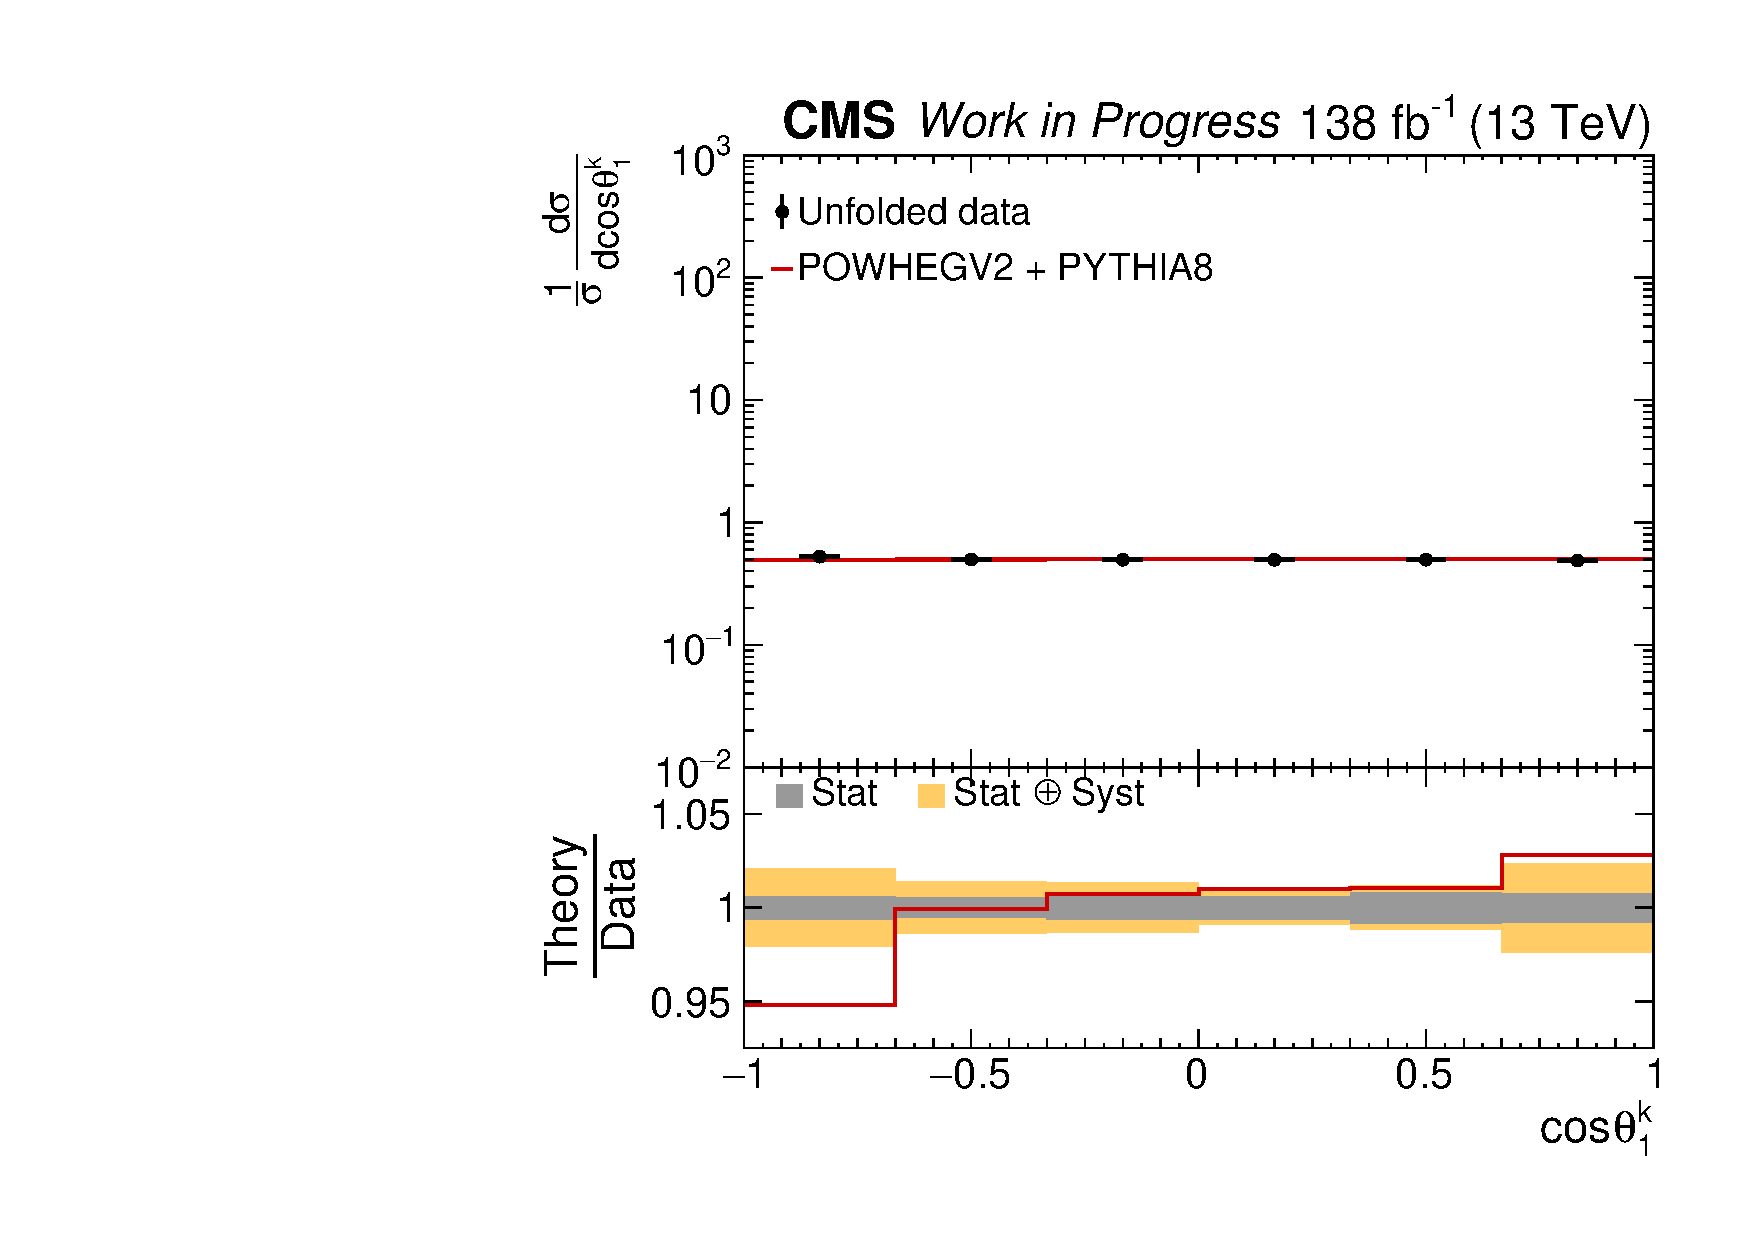
\includegraphics[width=0.40\textwidth]{fig_fullRun2UL/unfolding/combined/UnfoldedResultsNorm_b1k.pdf} \\
\label{fig:b1k}
\caption{Reconstructed detector-level distribution (Top Left), detector response-matrix (Top Right), absolute cross-section unfolded to parton-level (Bottom Left), and normalized cross-section unfolded to parton-level (Bottom Right) for polarization observable $\cos\theta_{1}^{k}$, from which spin-density coefficient $B_{1}^{k}$ (sensitive to spin-density coefficient function $b_k^{+}$) is extracted.}
\end{center}
\end{figure}
\clearpage
\begin{figure}[htb]
\begin{center}
 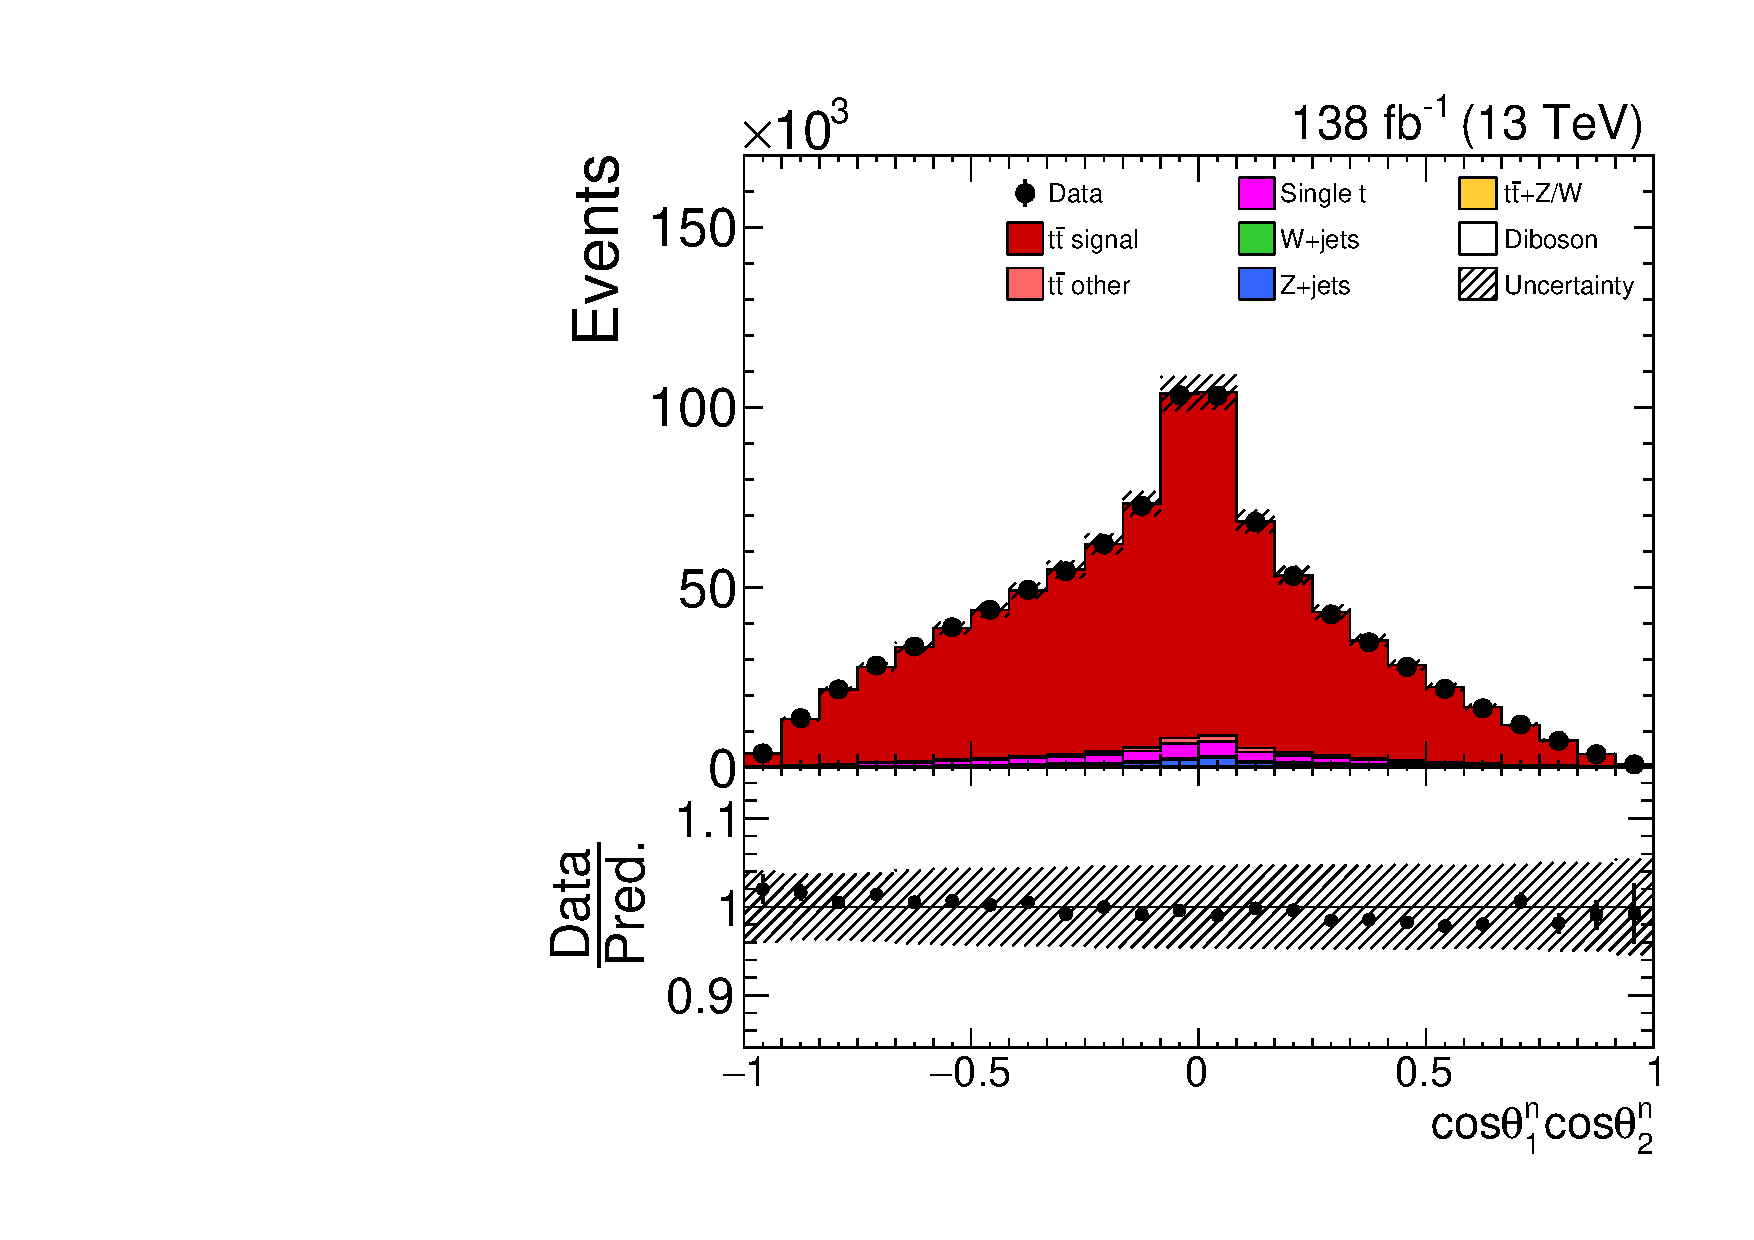
\includegraphics[width=0.40\textwidth]{fig_fullRun2UL/controlplots/combined/Hyp_LLBarCnn.pdf}
 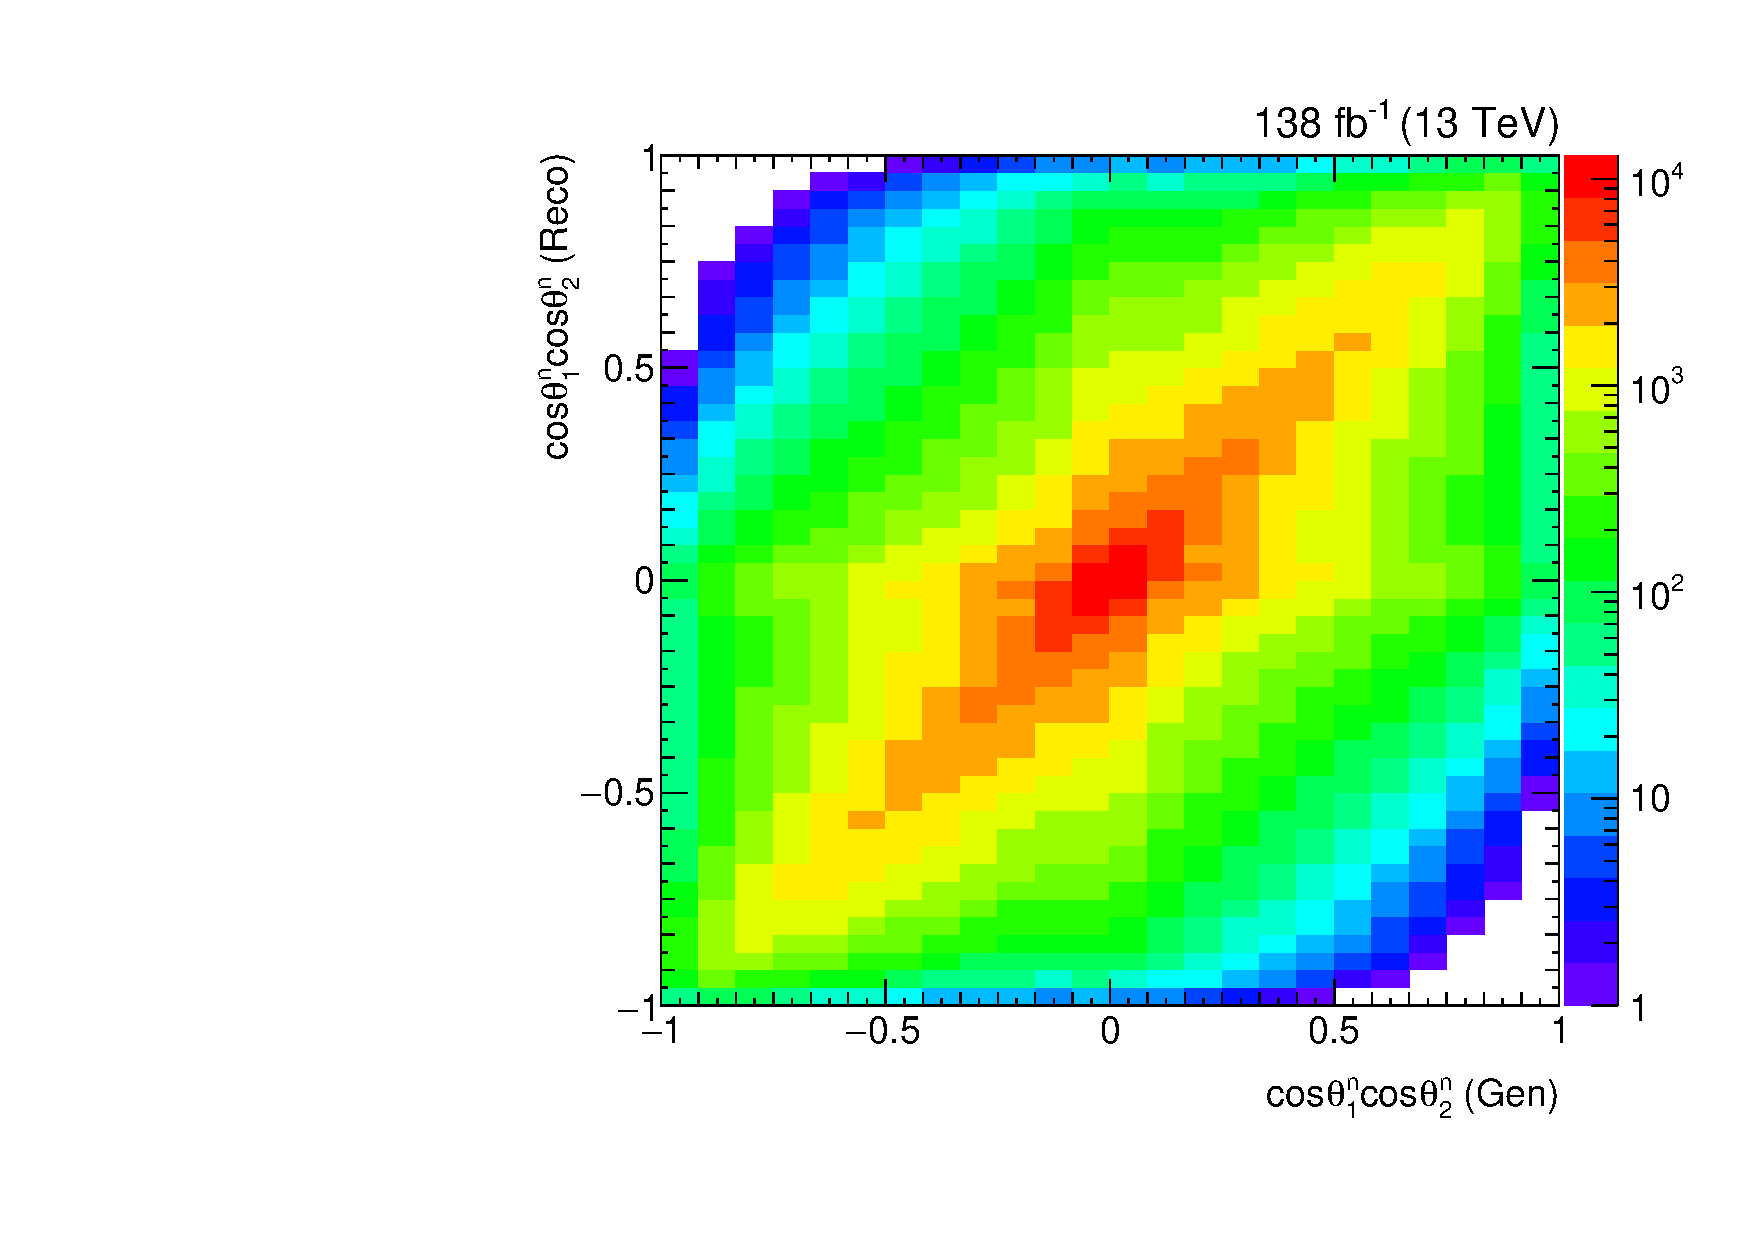
\includegraphics[width=0.40\textwidth]{fig_fullRun2UL/unfolding/combined/ResponseMatrix_c_nn.pdf} \\
 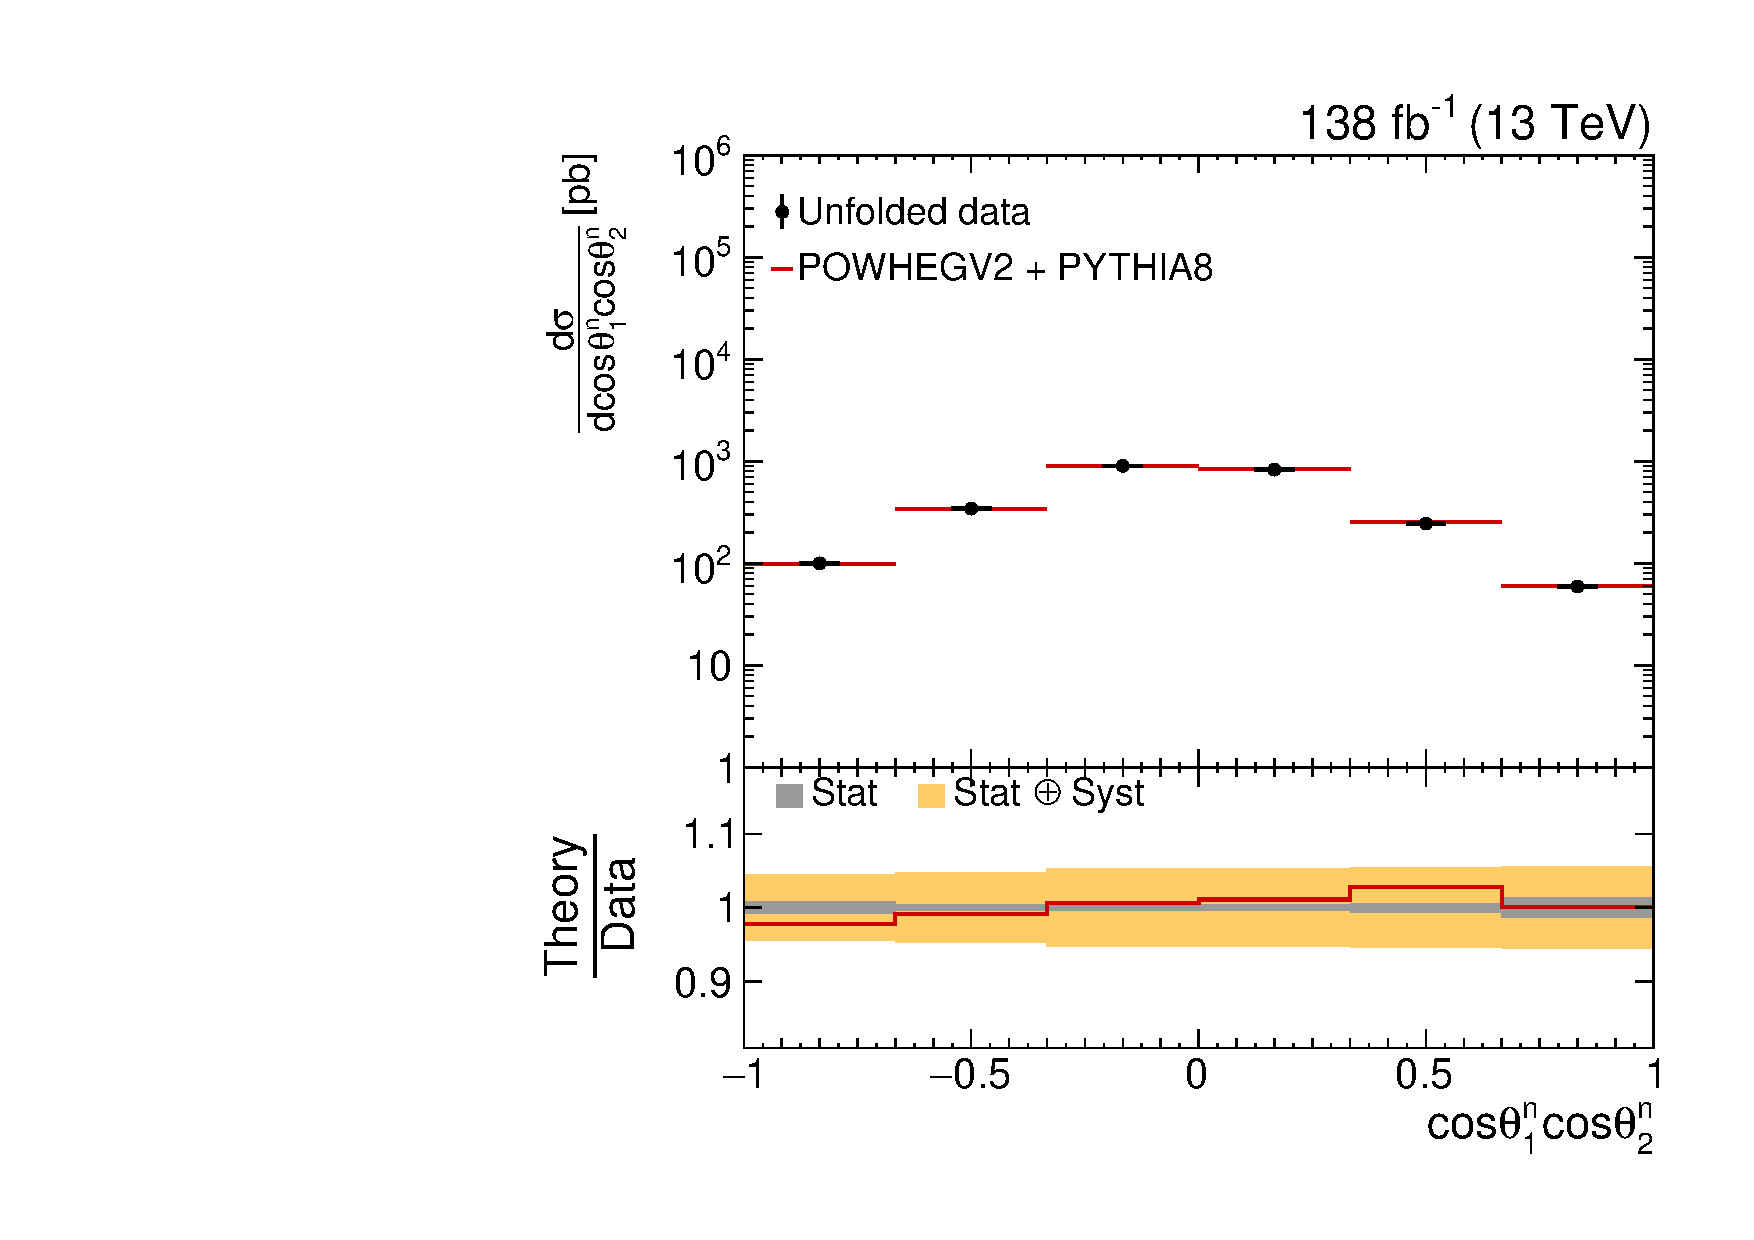
\includegraphics[width=0.40\textwidth]{fig_fullRun2UL/unfolding/combined/UnfoldedResults_c_nn.pdf}
 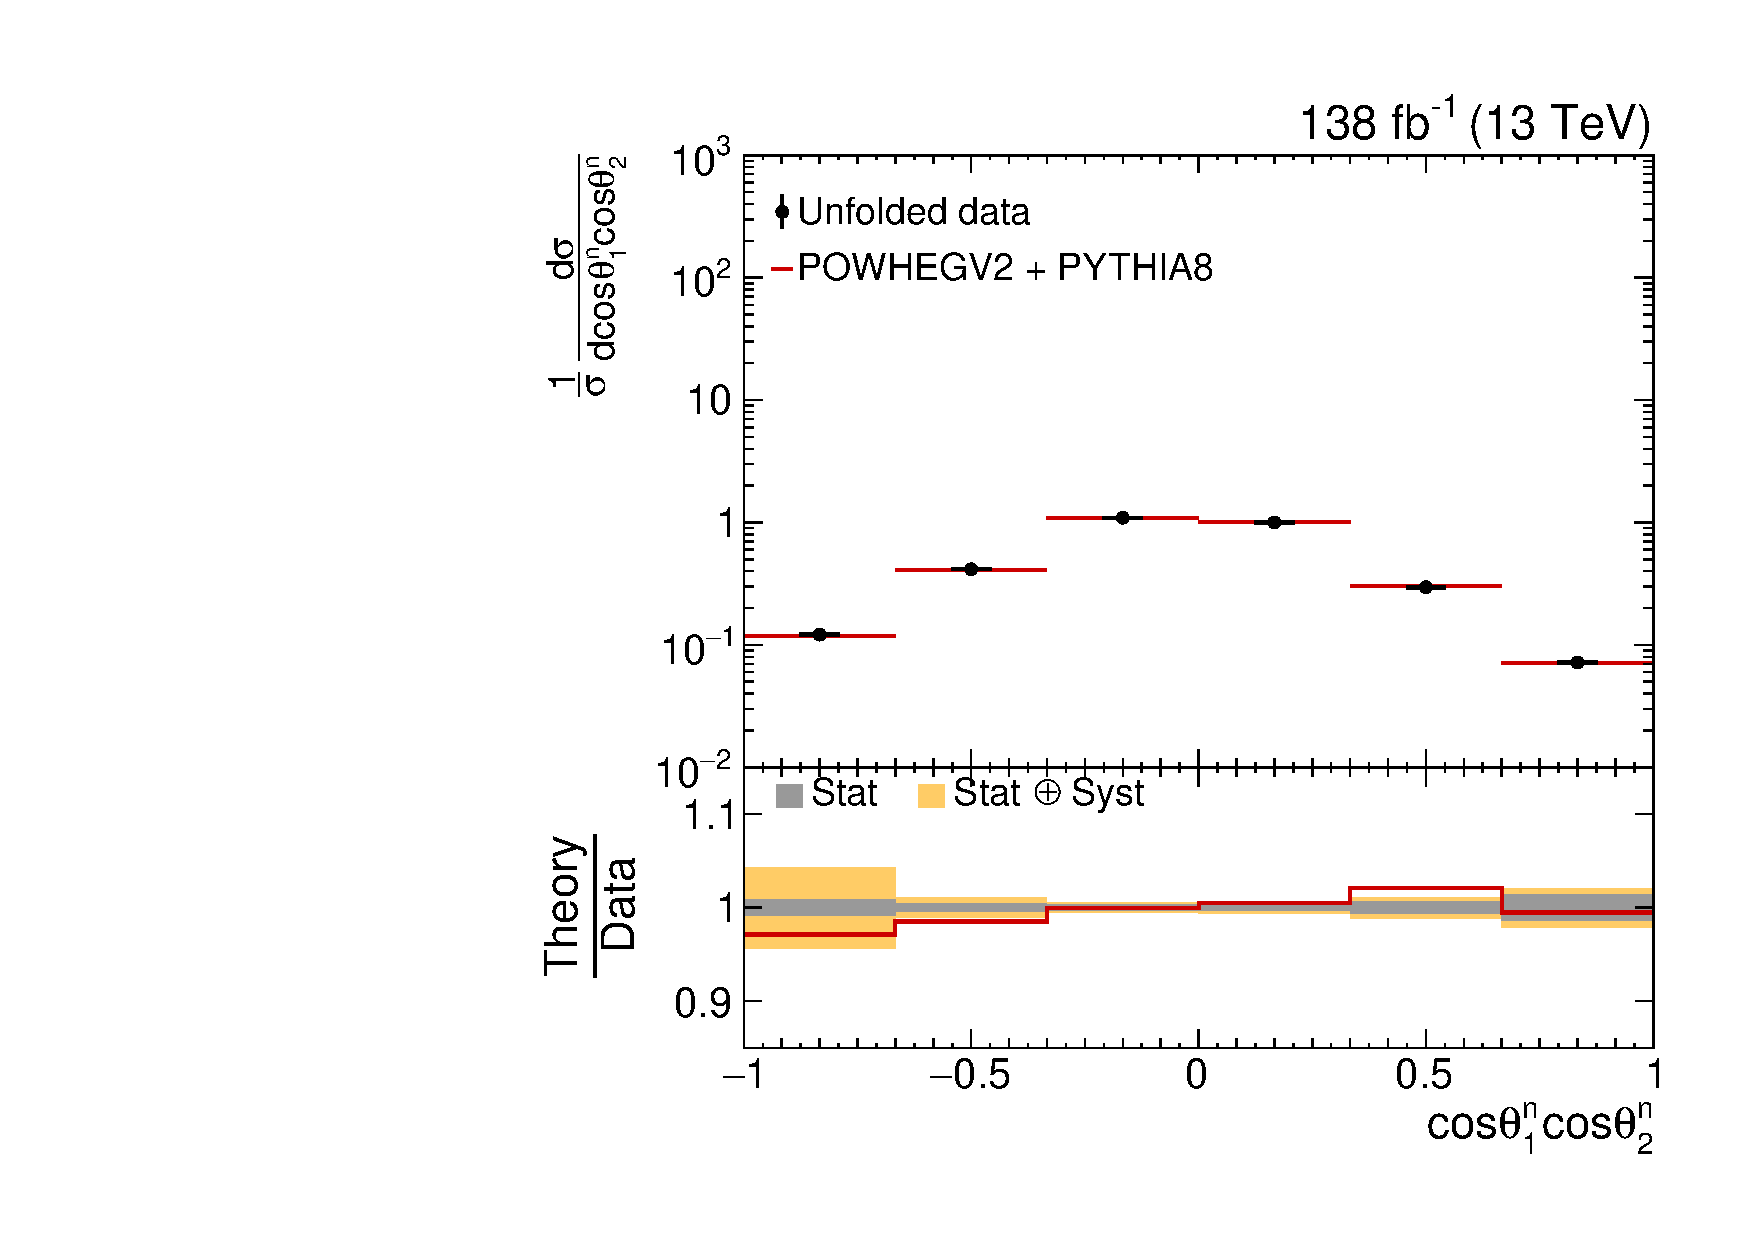
\includegraphics[width=0.40\textwidth]{fig_fullRun2UL/unfolding/combined/UnfoldedResultsNorm_c_nn.pdf} \\
\label{fig:c_nn}
\caption{Reconstructed detector-level distribution (Top Left), detector response-matrix (Top Right), absolute cross-section unfolded to parton-level (Bottom Left), and normalized cross-section unfolded to parton-level (Bottom Right) for diagonal spin correlation observable $\cos\theta_{1}^{n}\cos\theta_{2}^{n}$, from which spin-density coefficient $C_{nn}$ (sensitive to spin-density coefficient function $c_{n n}$) is extracted.}
\end{center}
\end{figure}
\clearpage
\begin{figure}[htb]
\begin{center}
 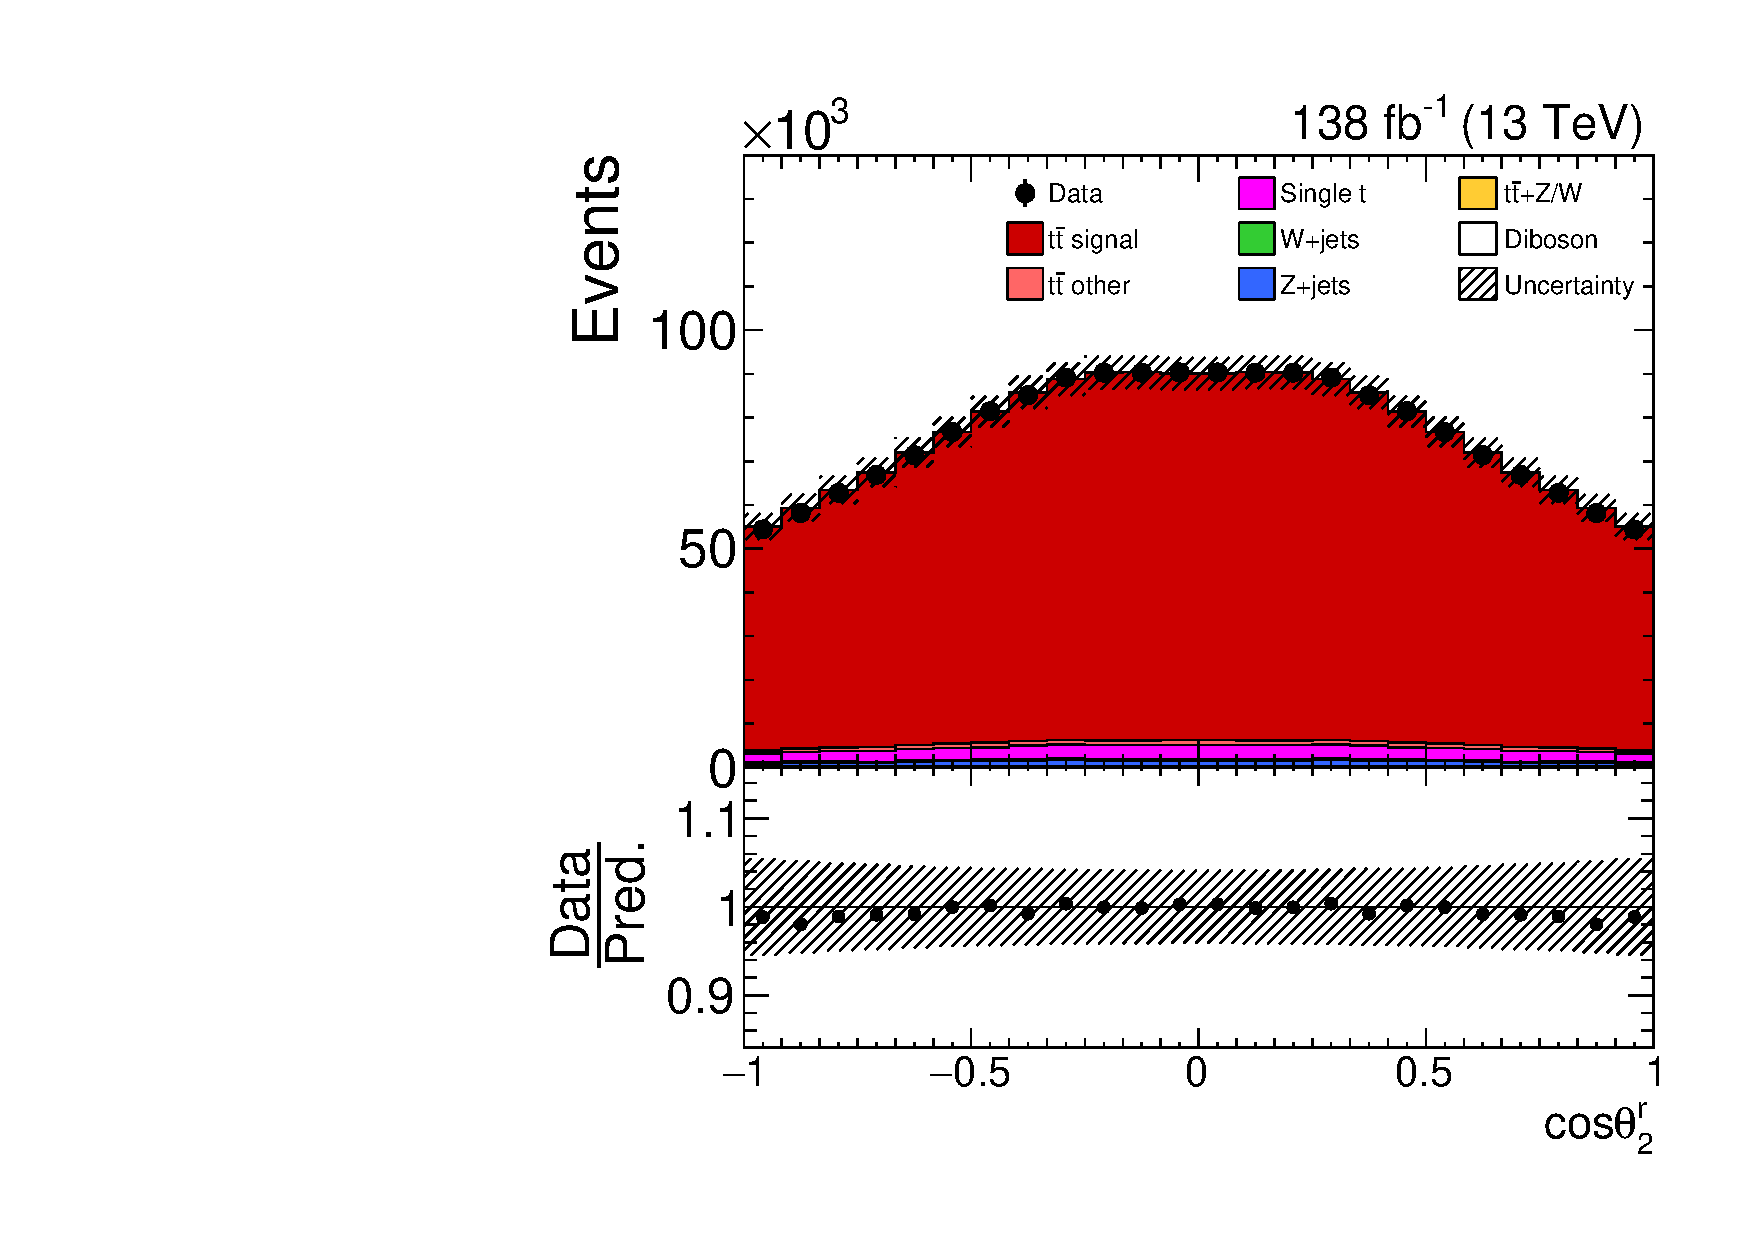
\includegraphics[width=0.40\textwidth]{fig_fullRun2UL/controlplots/combined/Hyp_LeptonBr.pdf}
 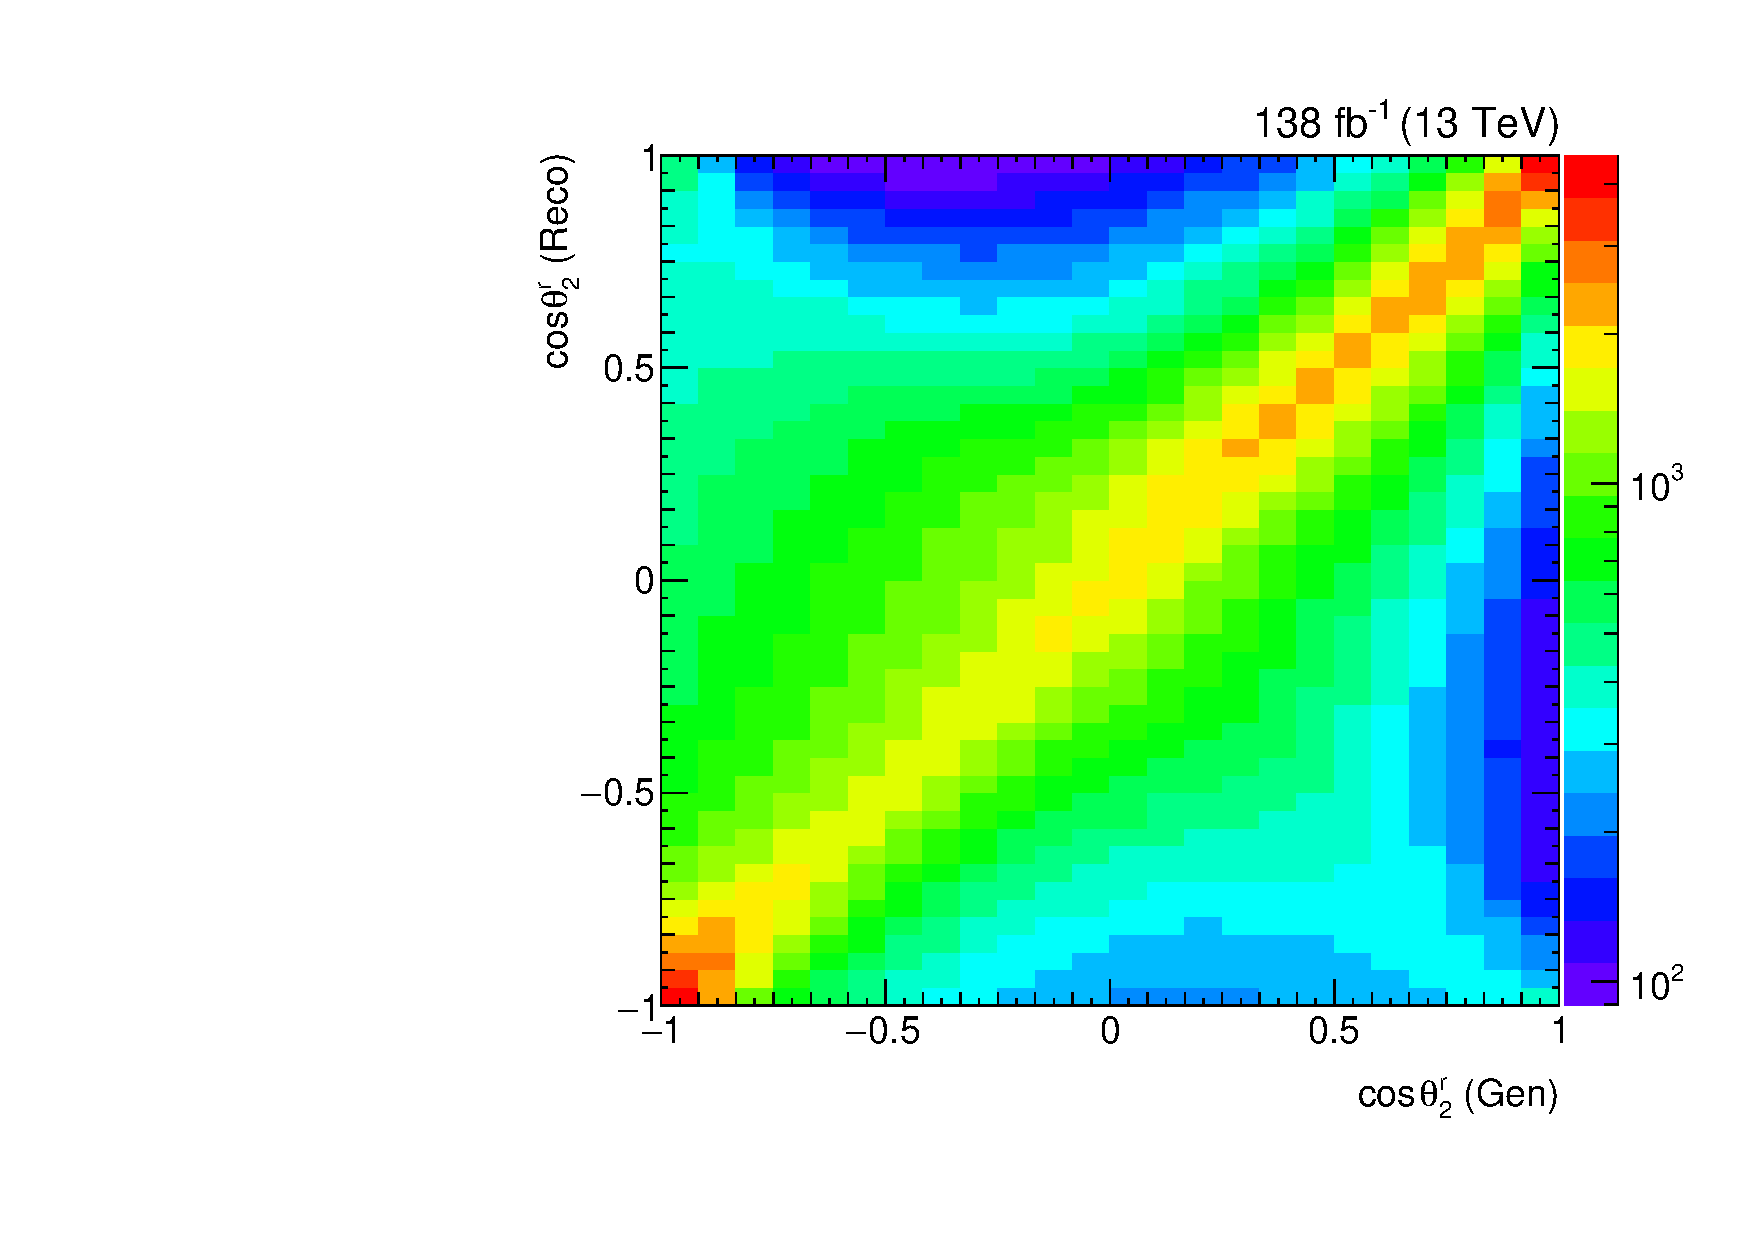
\includegraphics[width=0.40\textwidth]{fig_fullRun2UL/unfolding/combined/ResponseMatrix_b2r.pdf} \\
 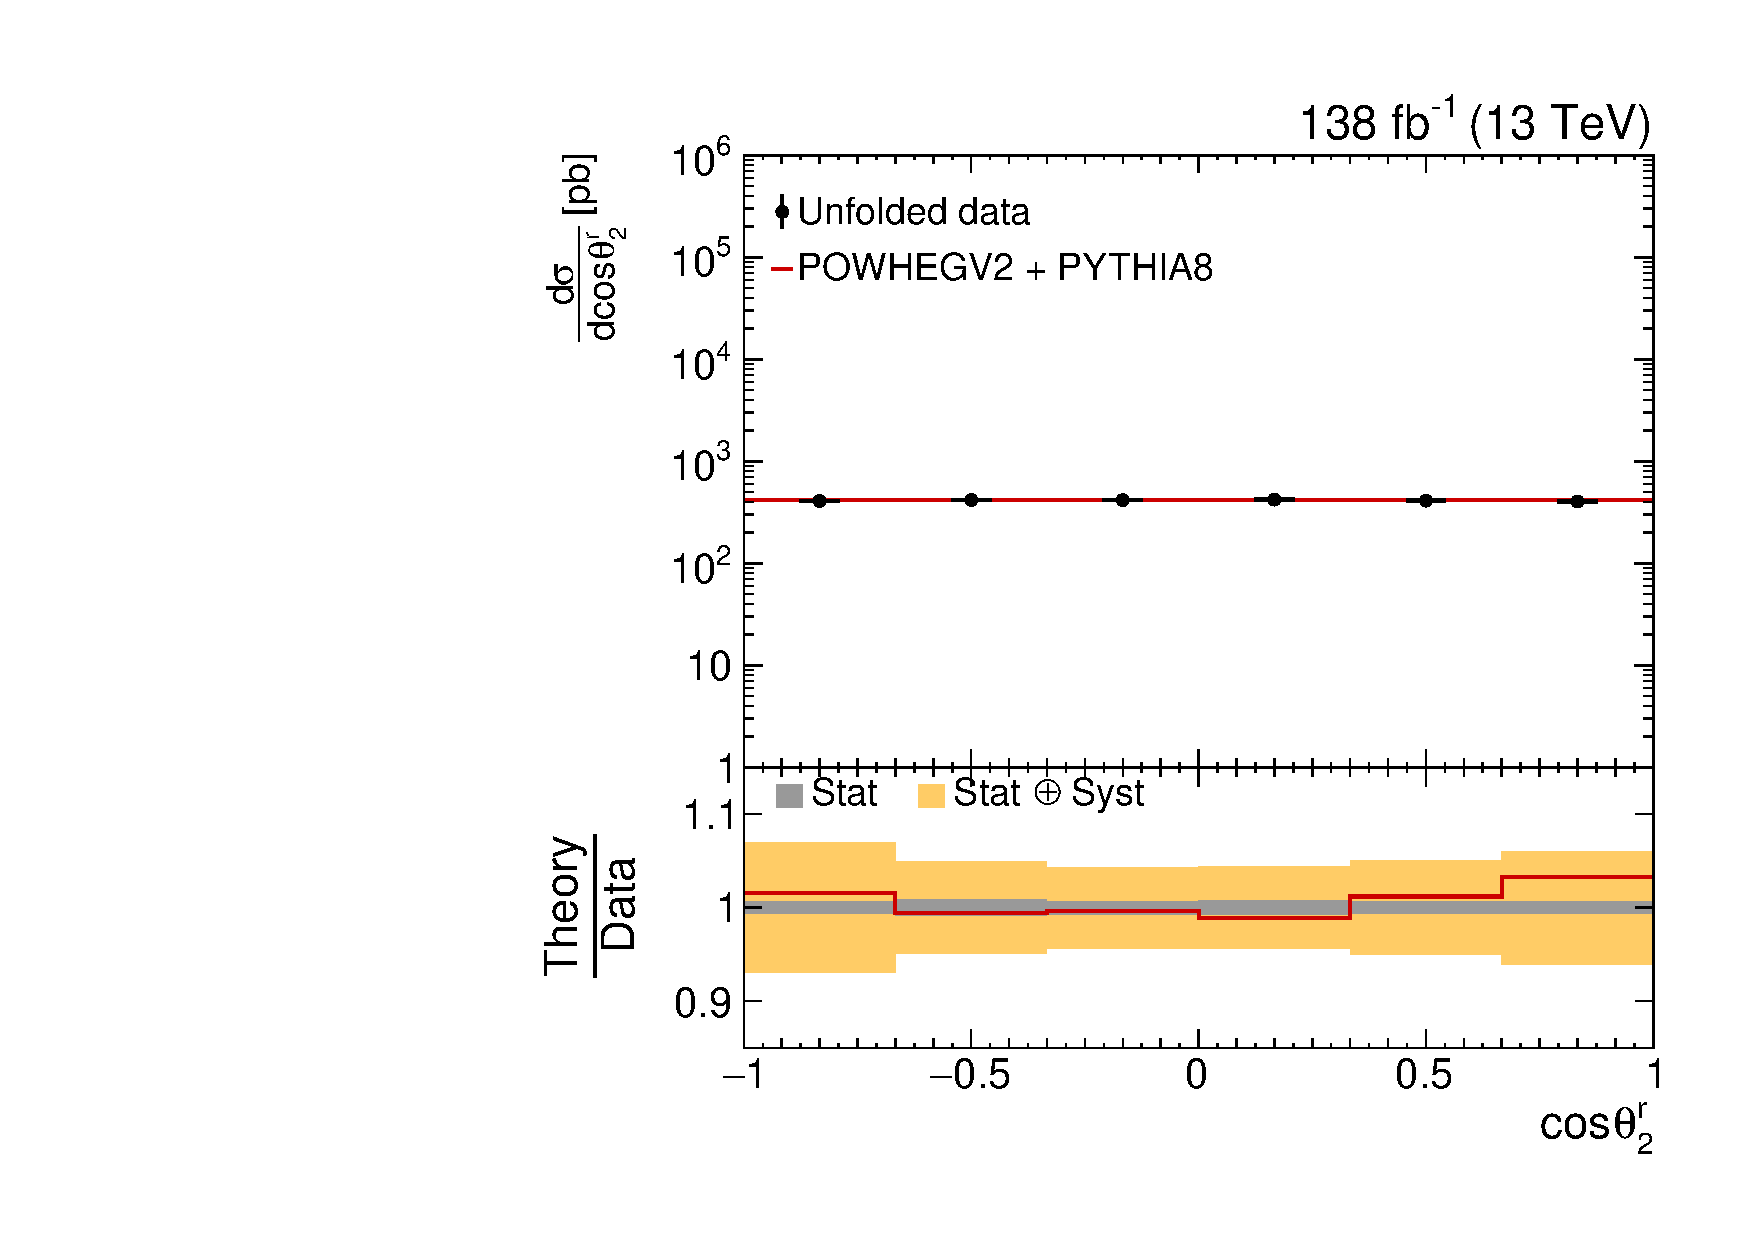
\includegraphics[width=0.40\textwidth]{fig_fullRun2UL/unfolding/combined/UnfoldedResults_b2r.pdf}
 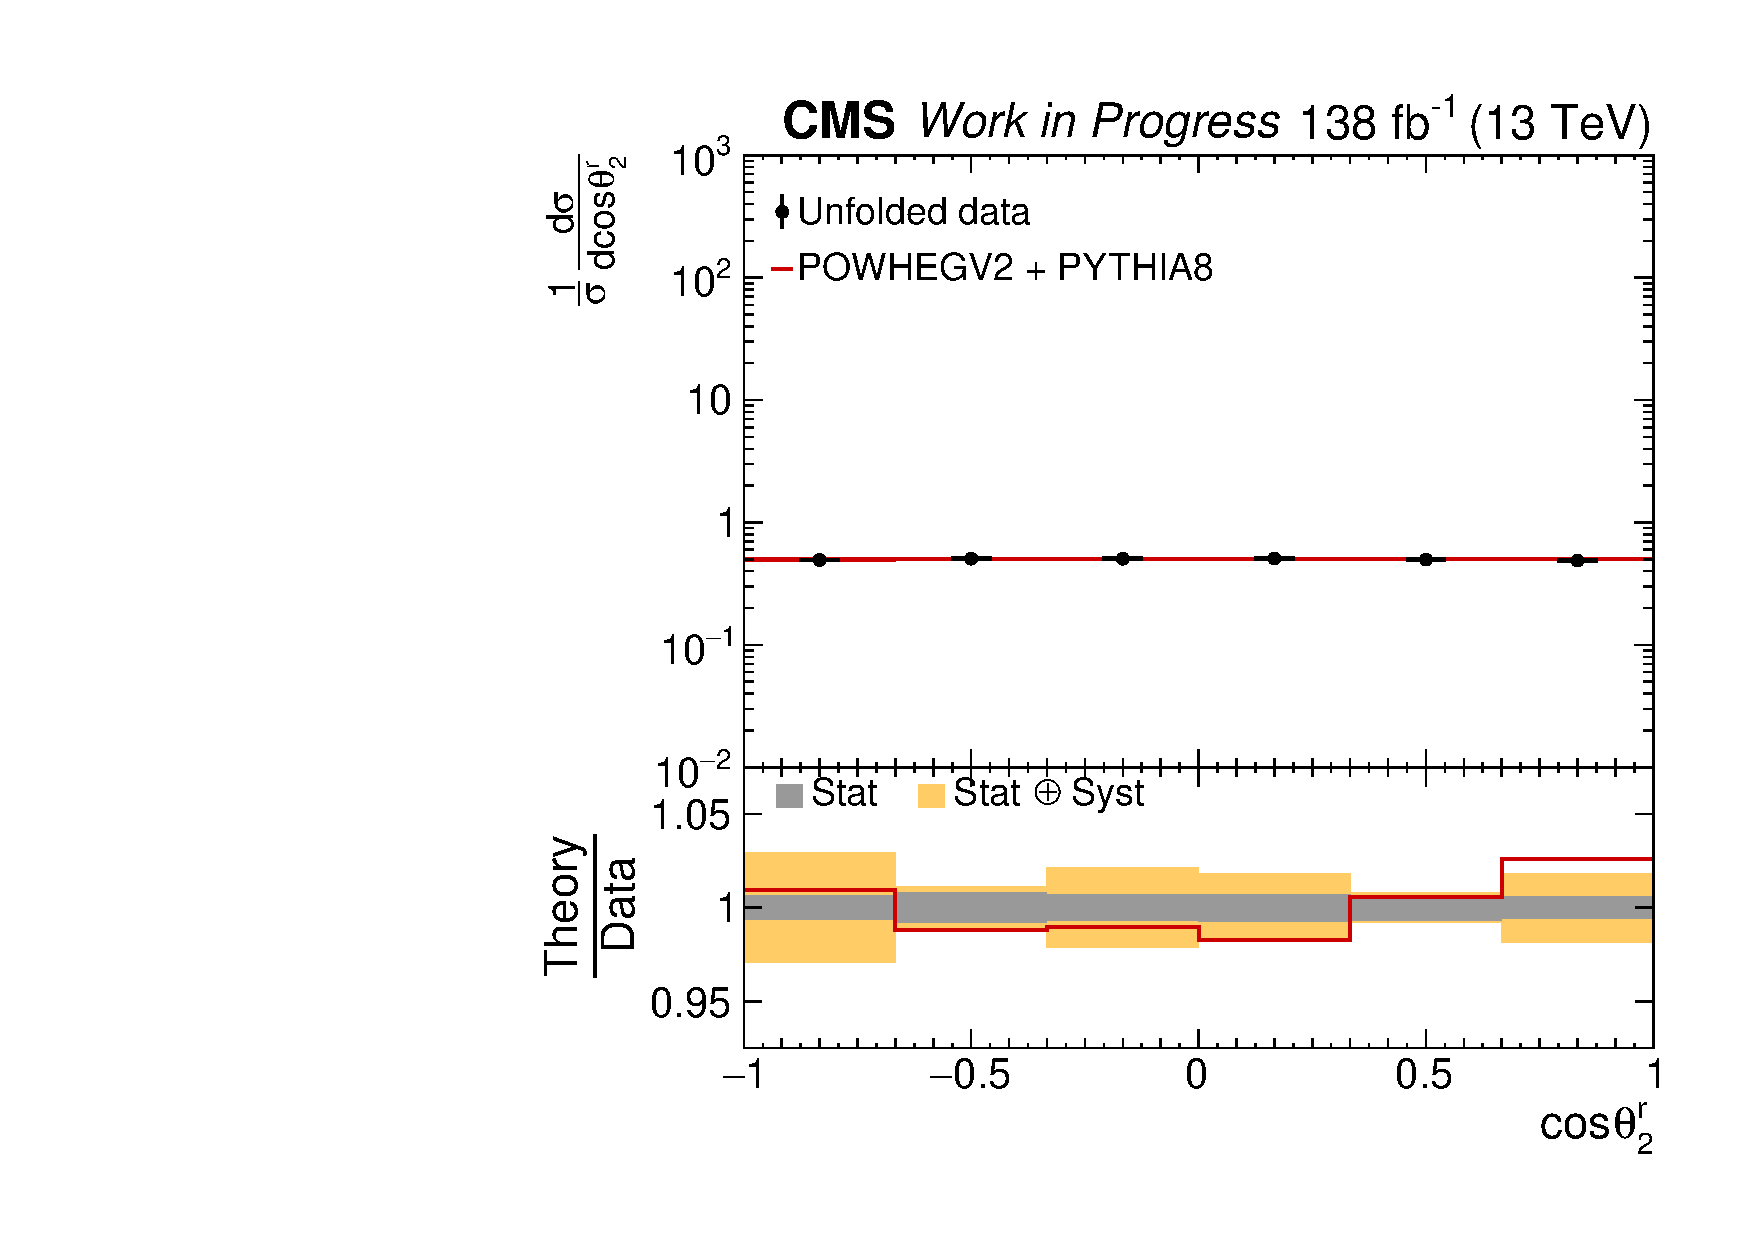
\includegraphics[width=0.40\textwidth]{fig_fullRun2UL/unfolding/combined/UnfoldedResultsNorm_b2r.pdf} \\
\label{fig:b2r}
\caption{Reconstructed detector-level distribution (Top Left), detector response-matrix (Top Right), absolute cross-section unfolded to parton-level (Bottom Left), and normalized cross-section unfolded to parton-level (Bottom Right) for polarization observable $\cos\theta_{2}^{r}$, from which spin-density coefficient $B_{2}^{r}$ (sensitive to spin-density coefficient function $b_r^{-}$) is extracted.}
\end{center}
\end{figure}
\clearpage
\begin{figure}[htb]
\begin{center}
 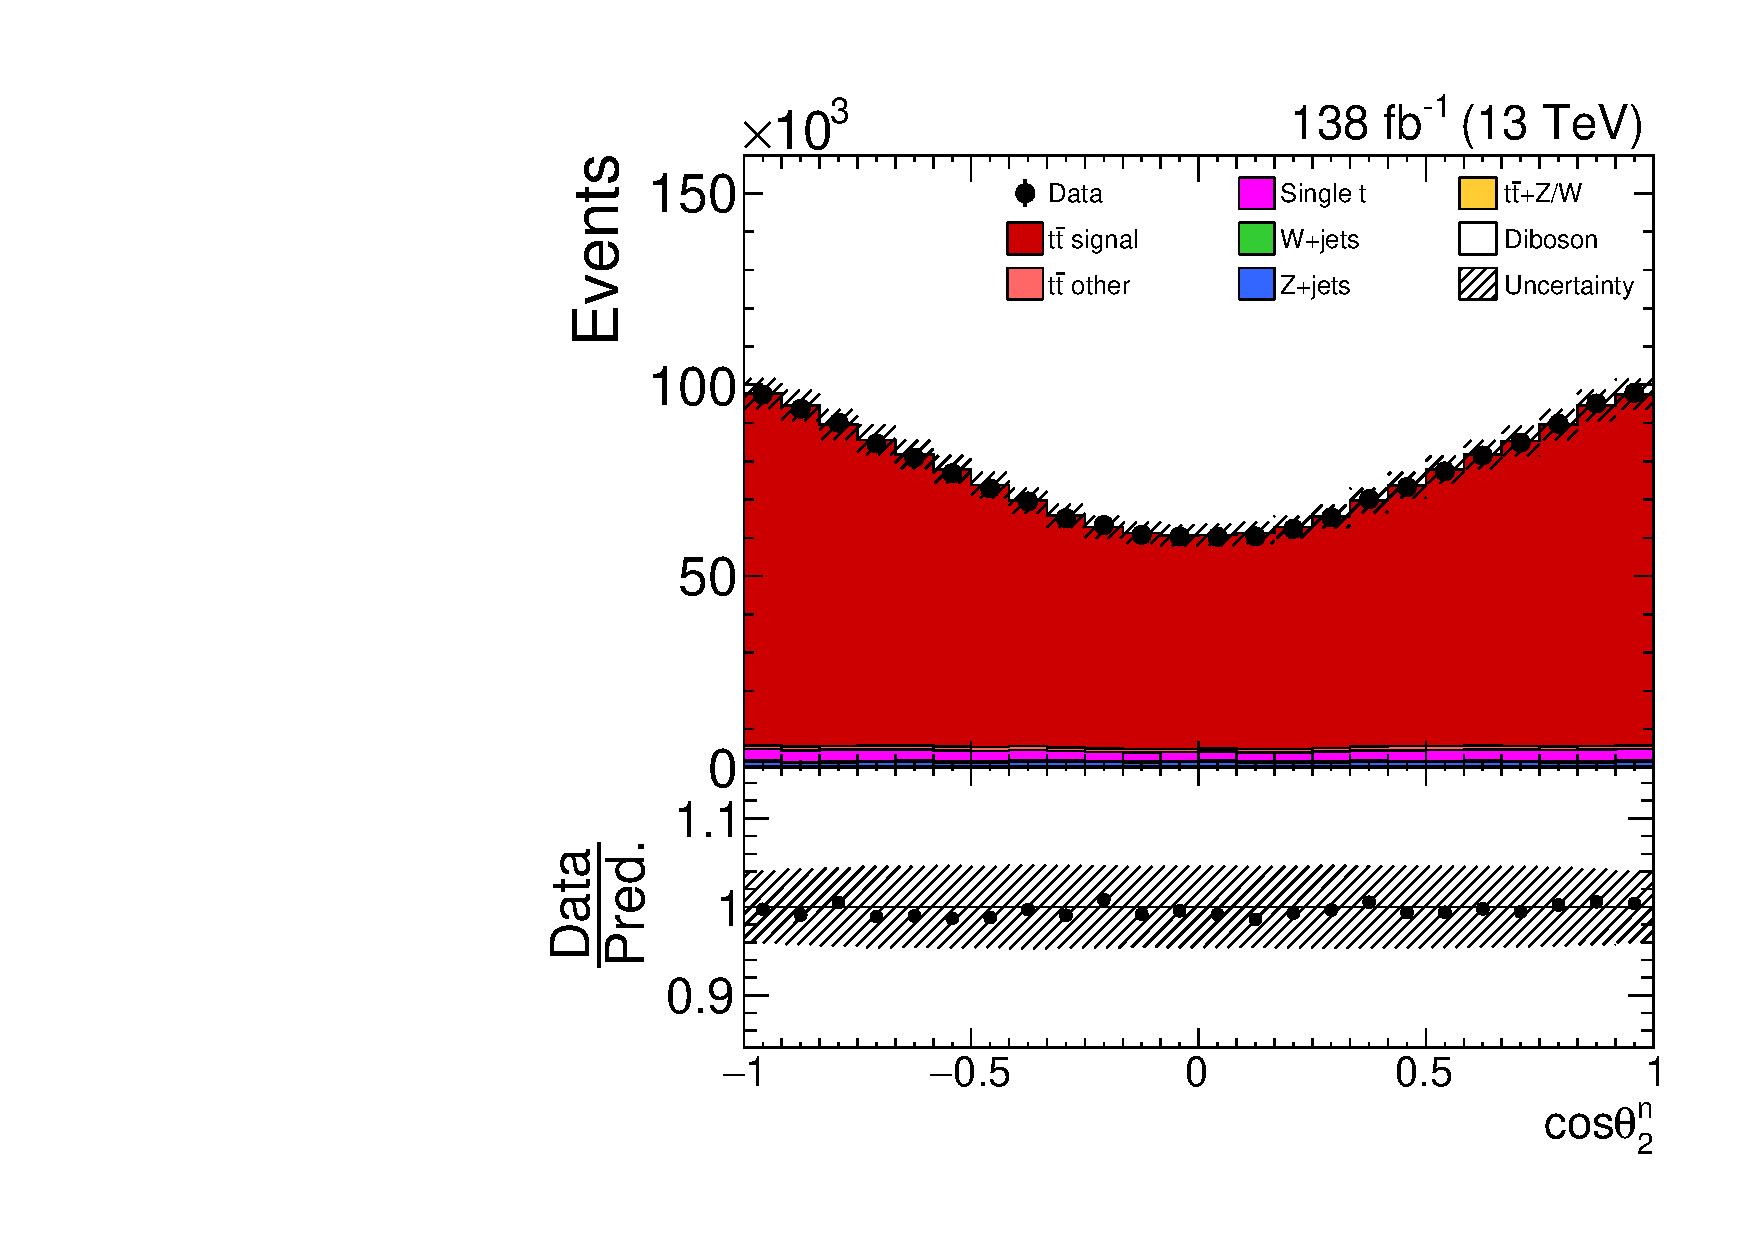
\includegraphics[width=0.40\textwidth]{fig_fullRun2UL/controlplots/combined/Hyp_LeptonBn.pdf}
 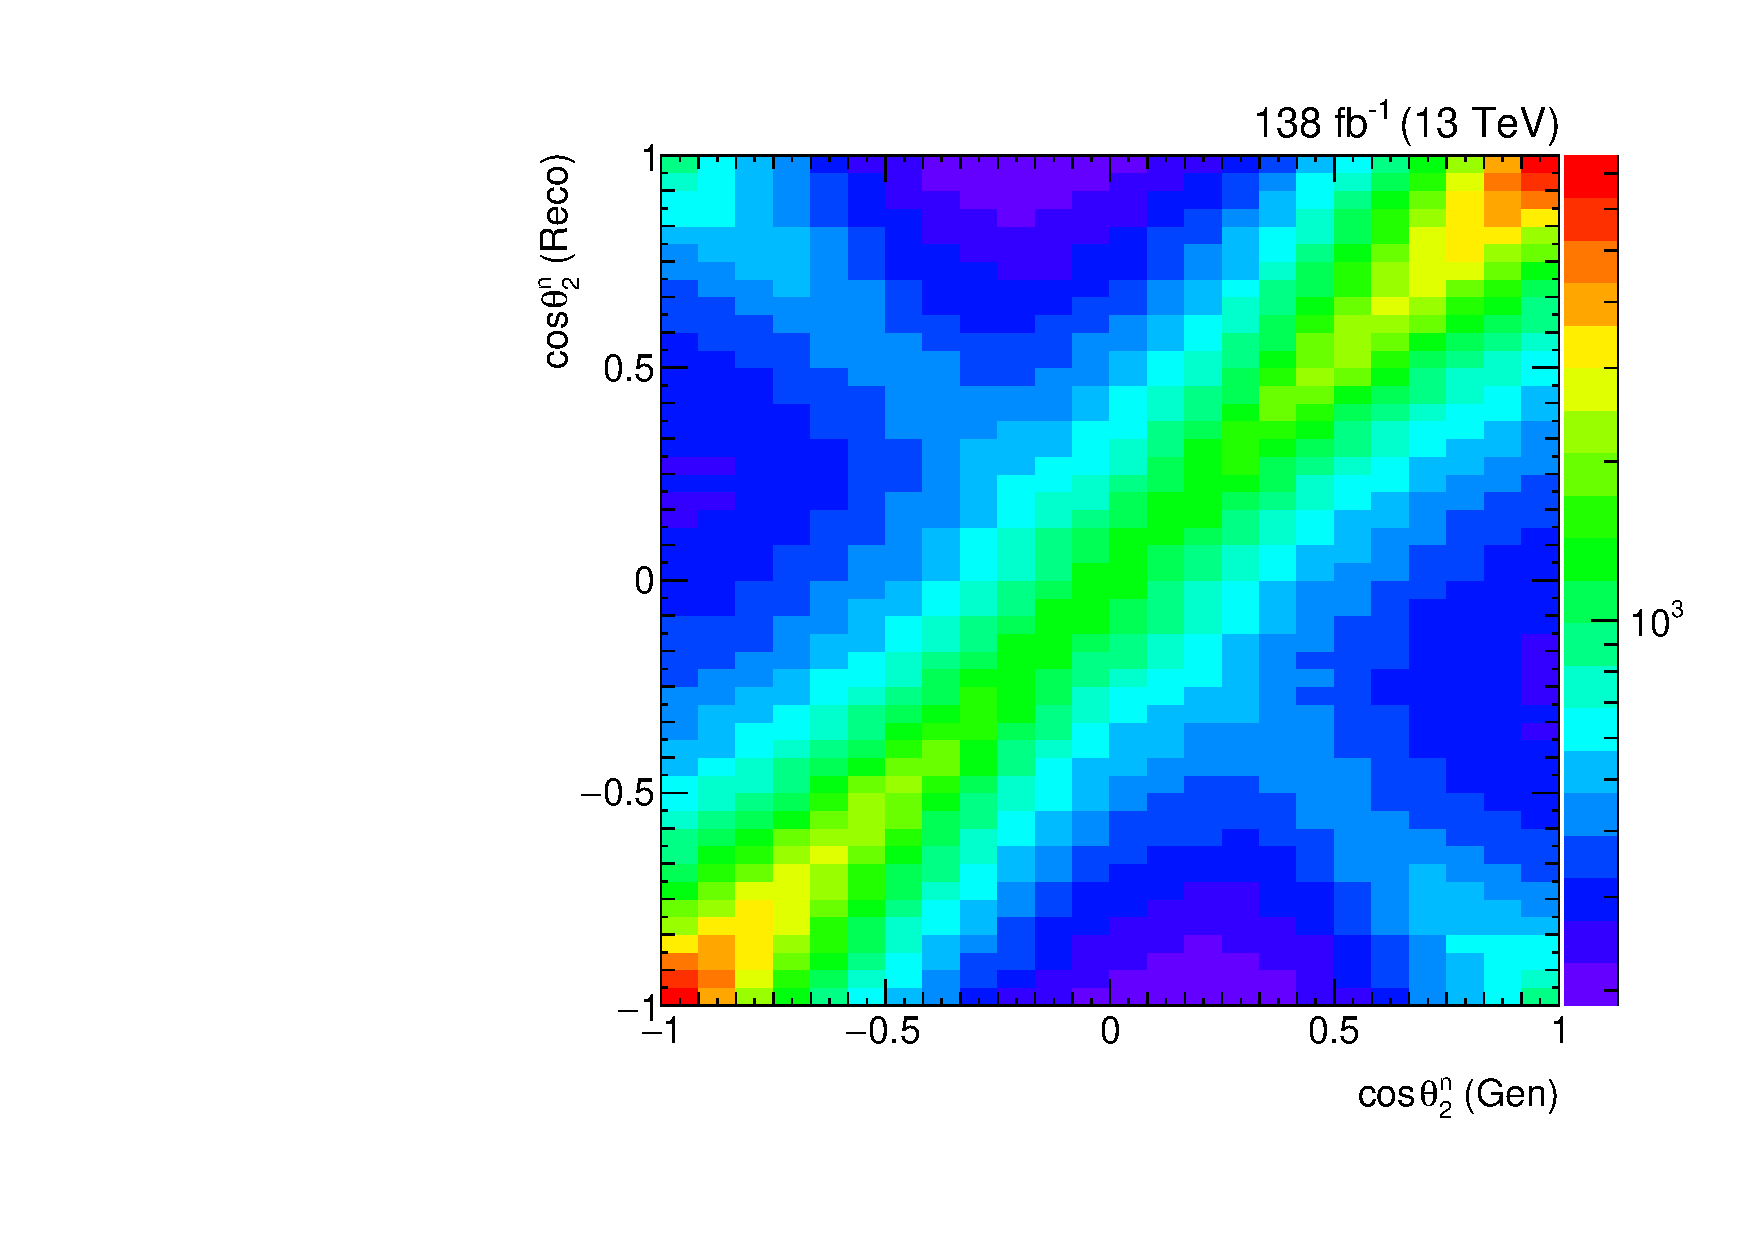
\includegraphics[width=0.40\textwidth]{fig_fullRun2UL/unfolding/combined/ResponseMatrix_b2n.pdf} \\
 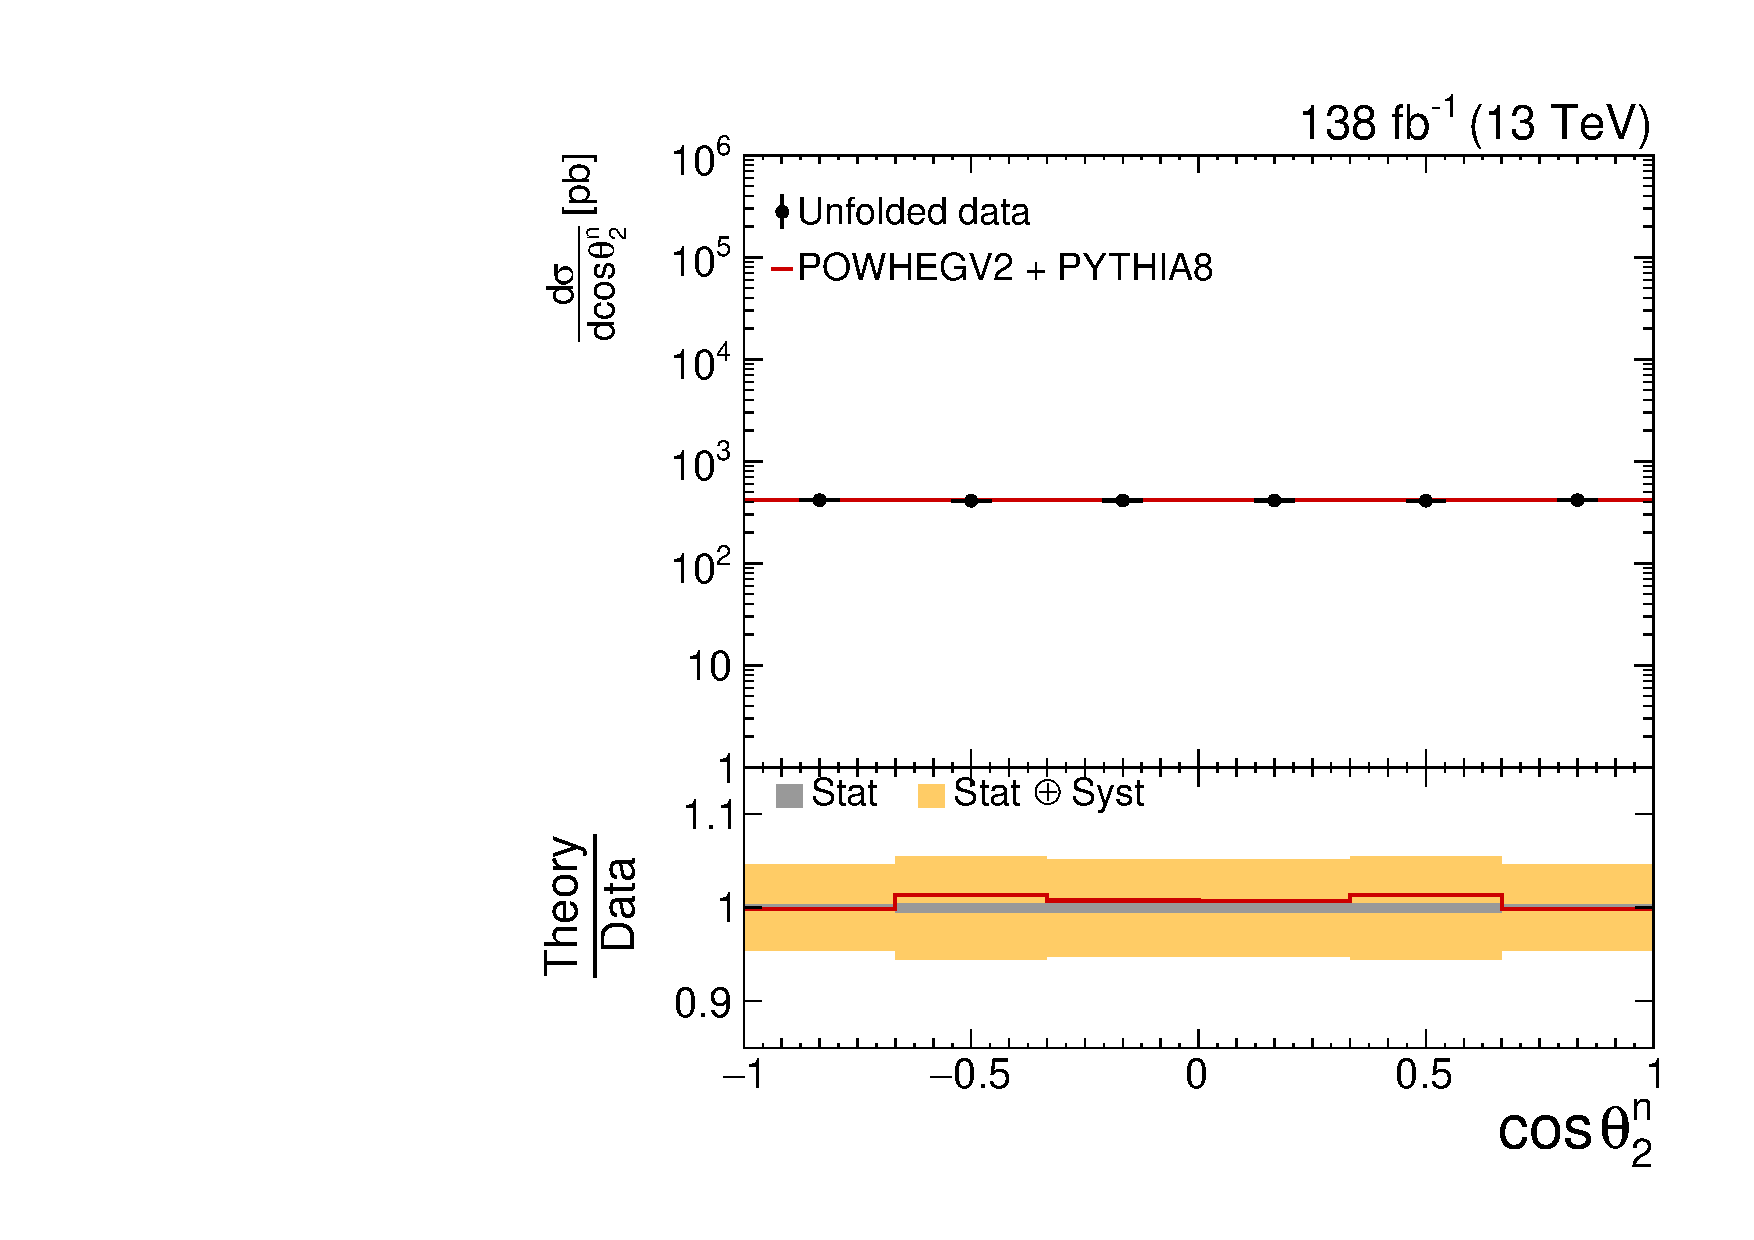
\includegraphics[width=0.40\textwidth]{fig_fullRun2UL/unfolding/combined/UnfoldedResults_b2n.pdf}
 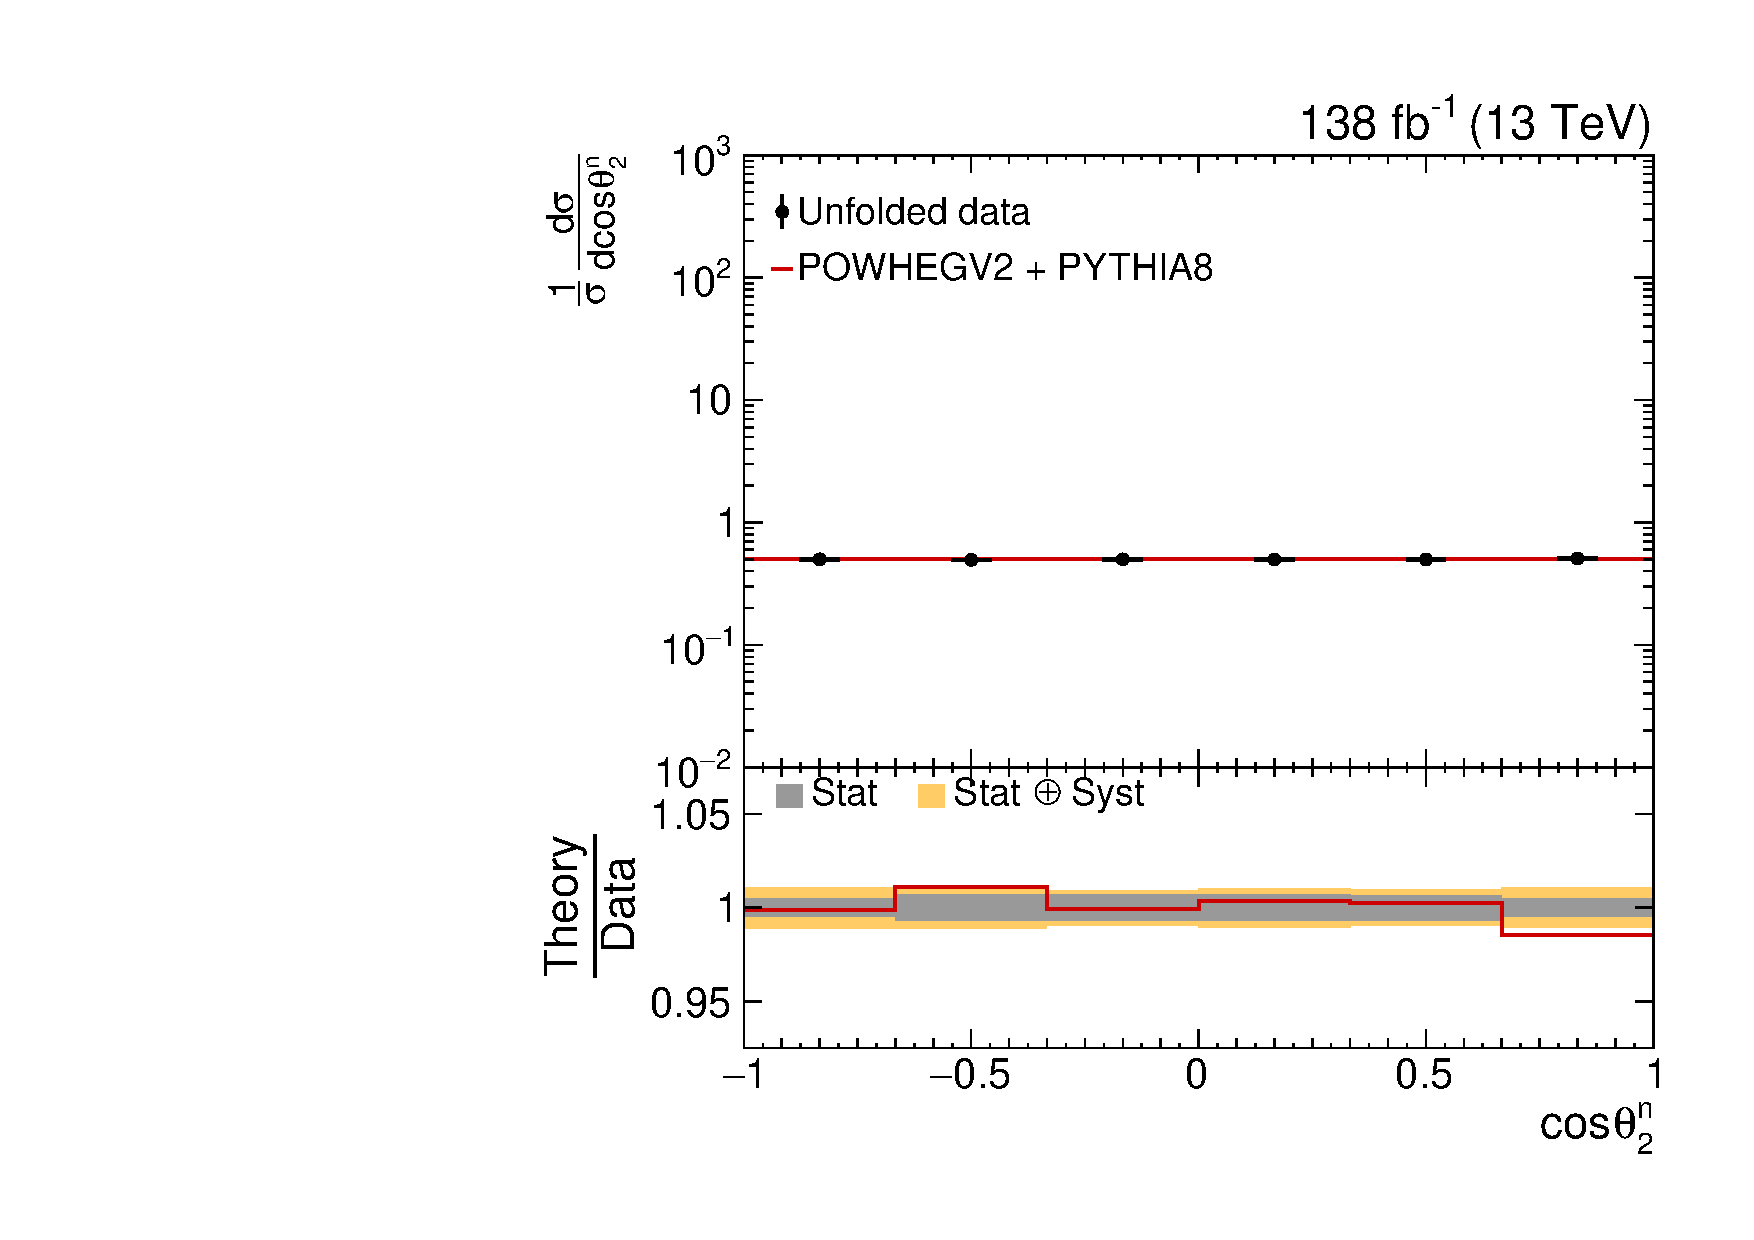
\includegraphics[width=0.40\textwidth]{fig_fullRun2UL/unfolding/combined/UnfoldedResultsNorm_b2n.pdf} \\
\label{fig:b2n}
\caption{Reconstructed detector-level distribution (Top Left), detector response-matrix (Top Right), absolute cross-section unfolded to parton-level (Bottom Left), and normalized cross-section unfolded to parton-level (Bottom Right) for polarization observable $\cos\theta_{2}^{n}$, from which spin-density coefficient $B_{2}^{n}$ (sensitive to spin-density coefficient function $b_n^{-}$) is extracted.}
\end{center}
\end{figure}
\clearpage
\begin{figure}[htb]
\begin{center}
 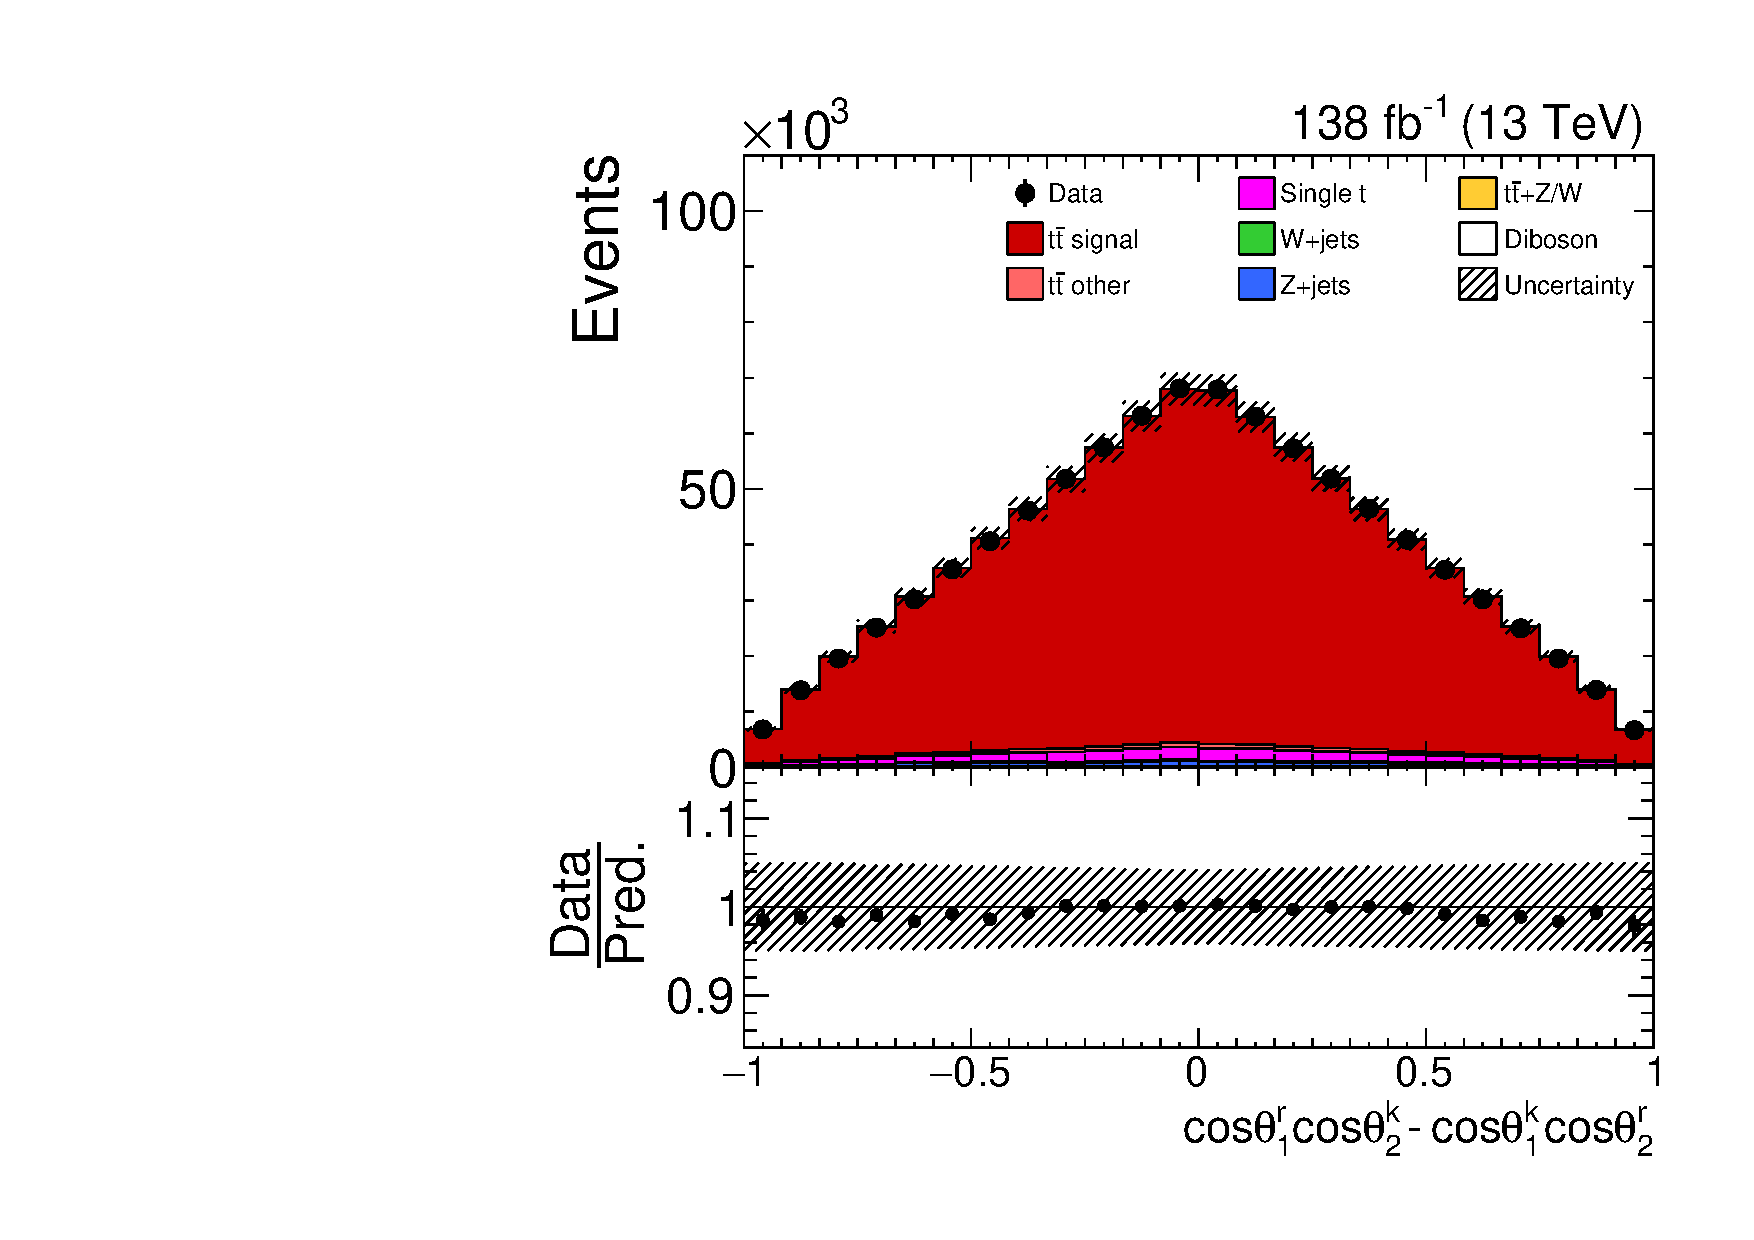
\includegraphics[width=0.40\textwidth]{fig_fullRun2UL/controlplots/combined/Hyp_LLBarCMrk.pdf}
 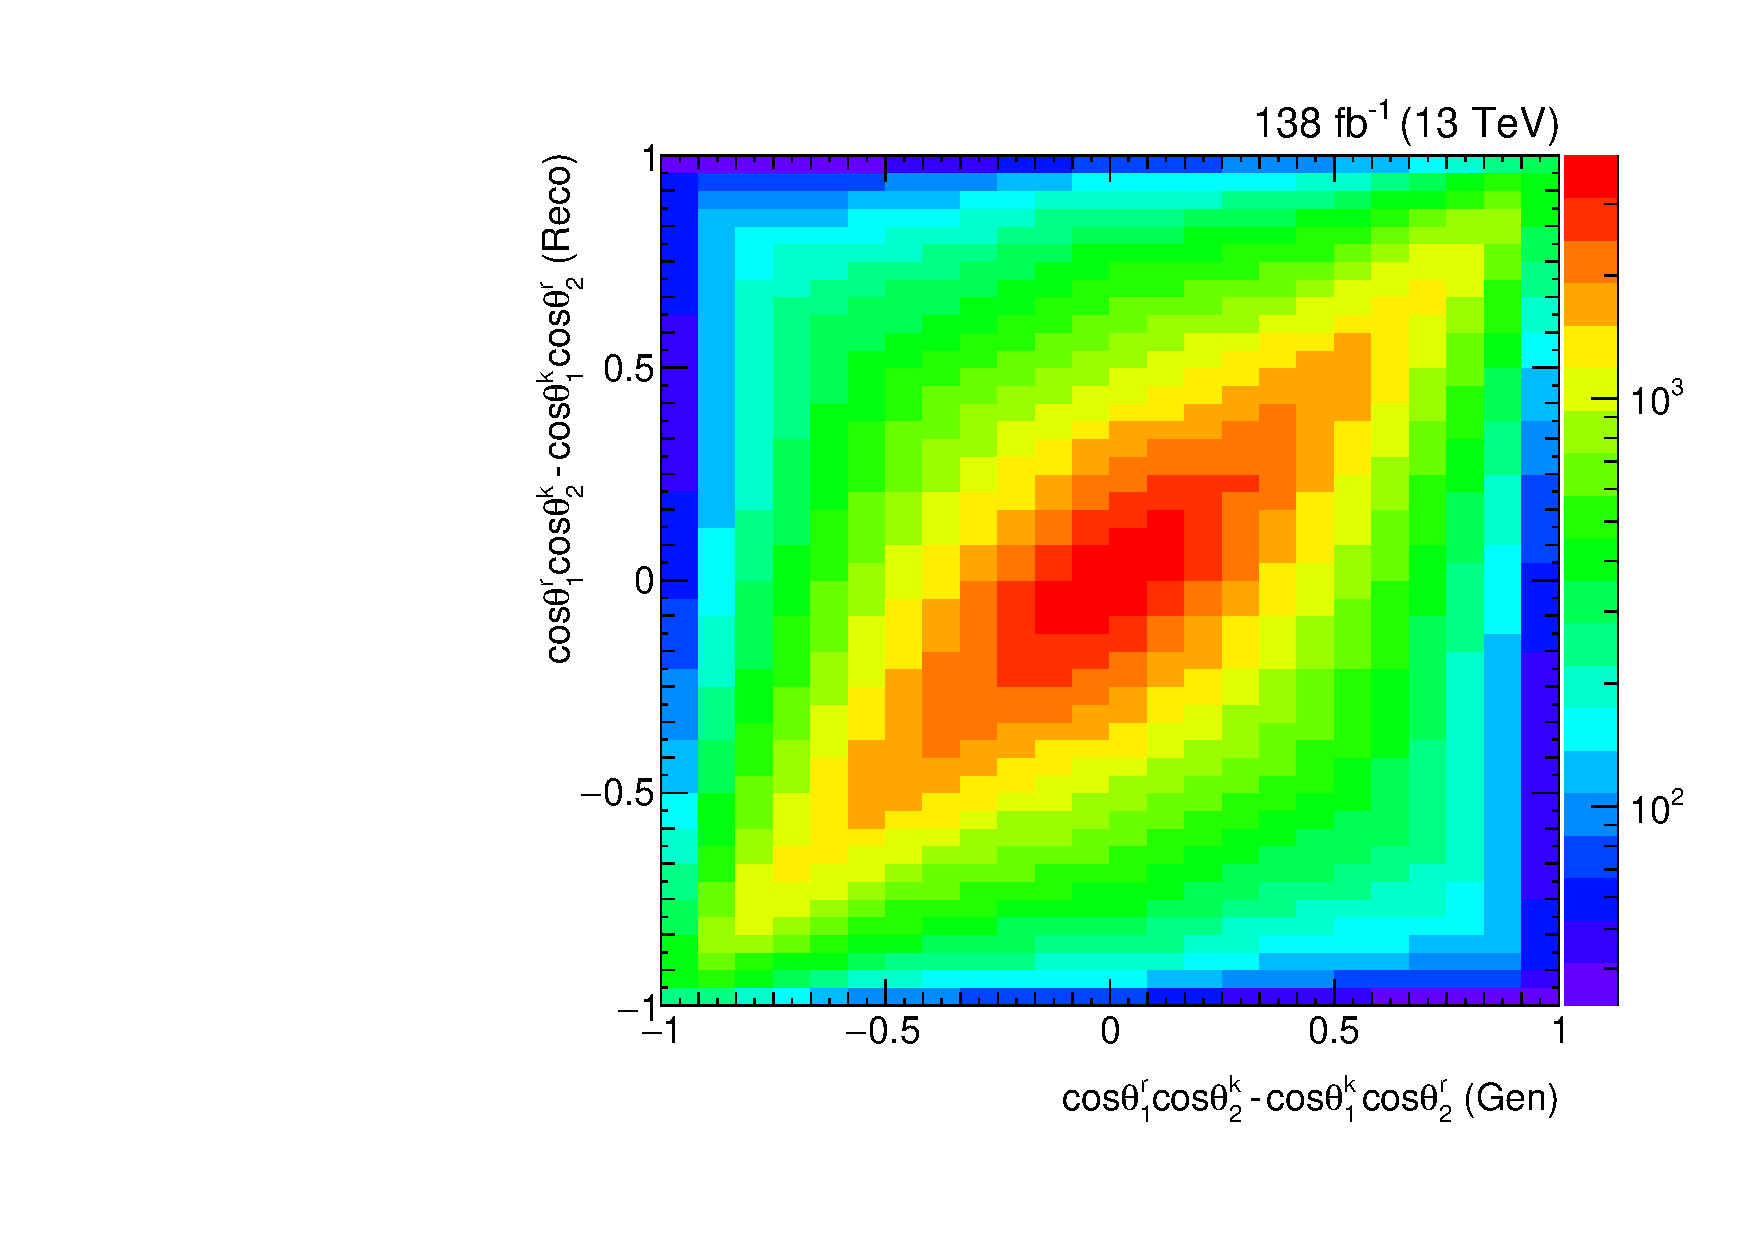
\includegraphics[width=0.40\textwidth]{fig_fullRun2UL/unfolding/combined/ResponseMatrix_c_Mrk.pdf} \\
 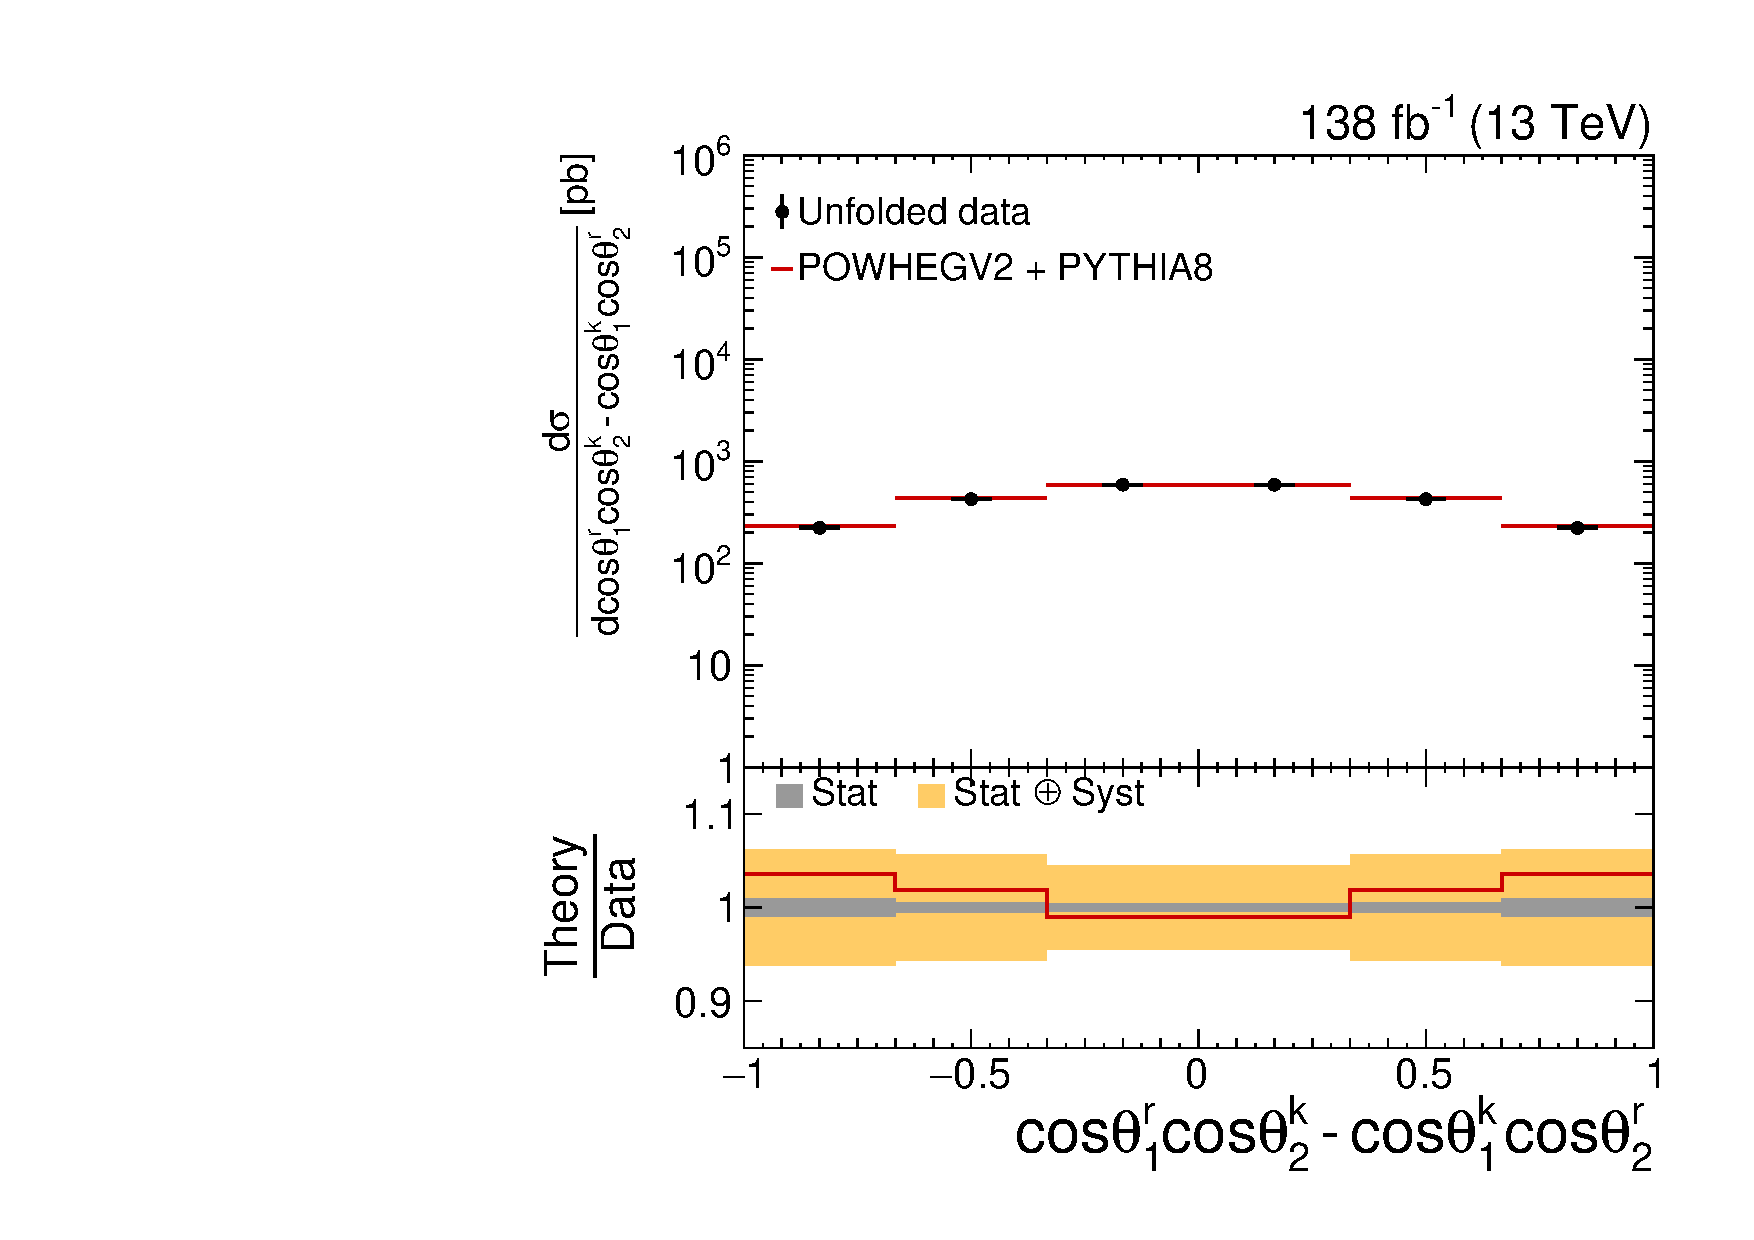
\includegraphics[width=0.40\textwidth]{fig_fullRun2UL/unfolding/combined/UnfoldedResults_c_Mrk.pdf}
 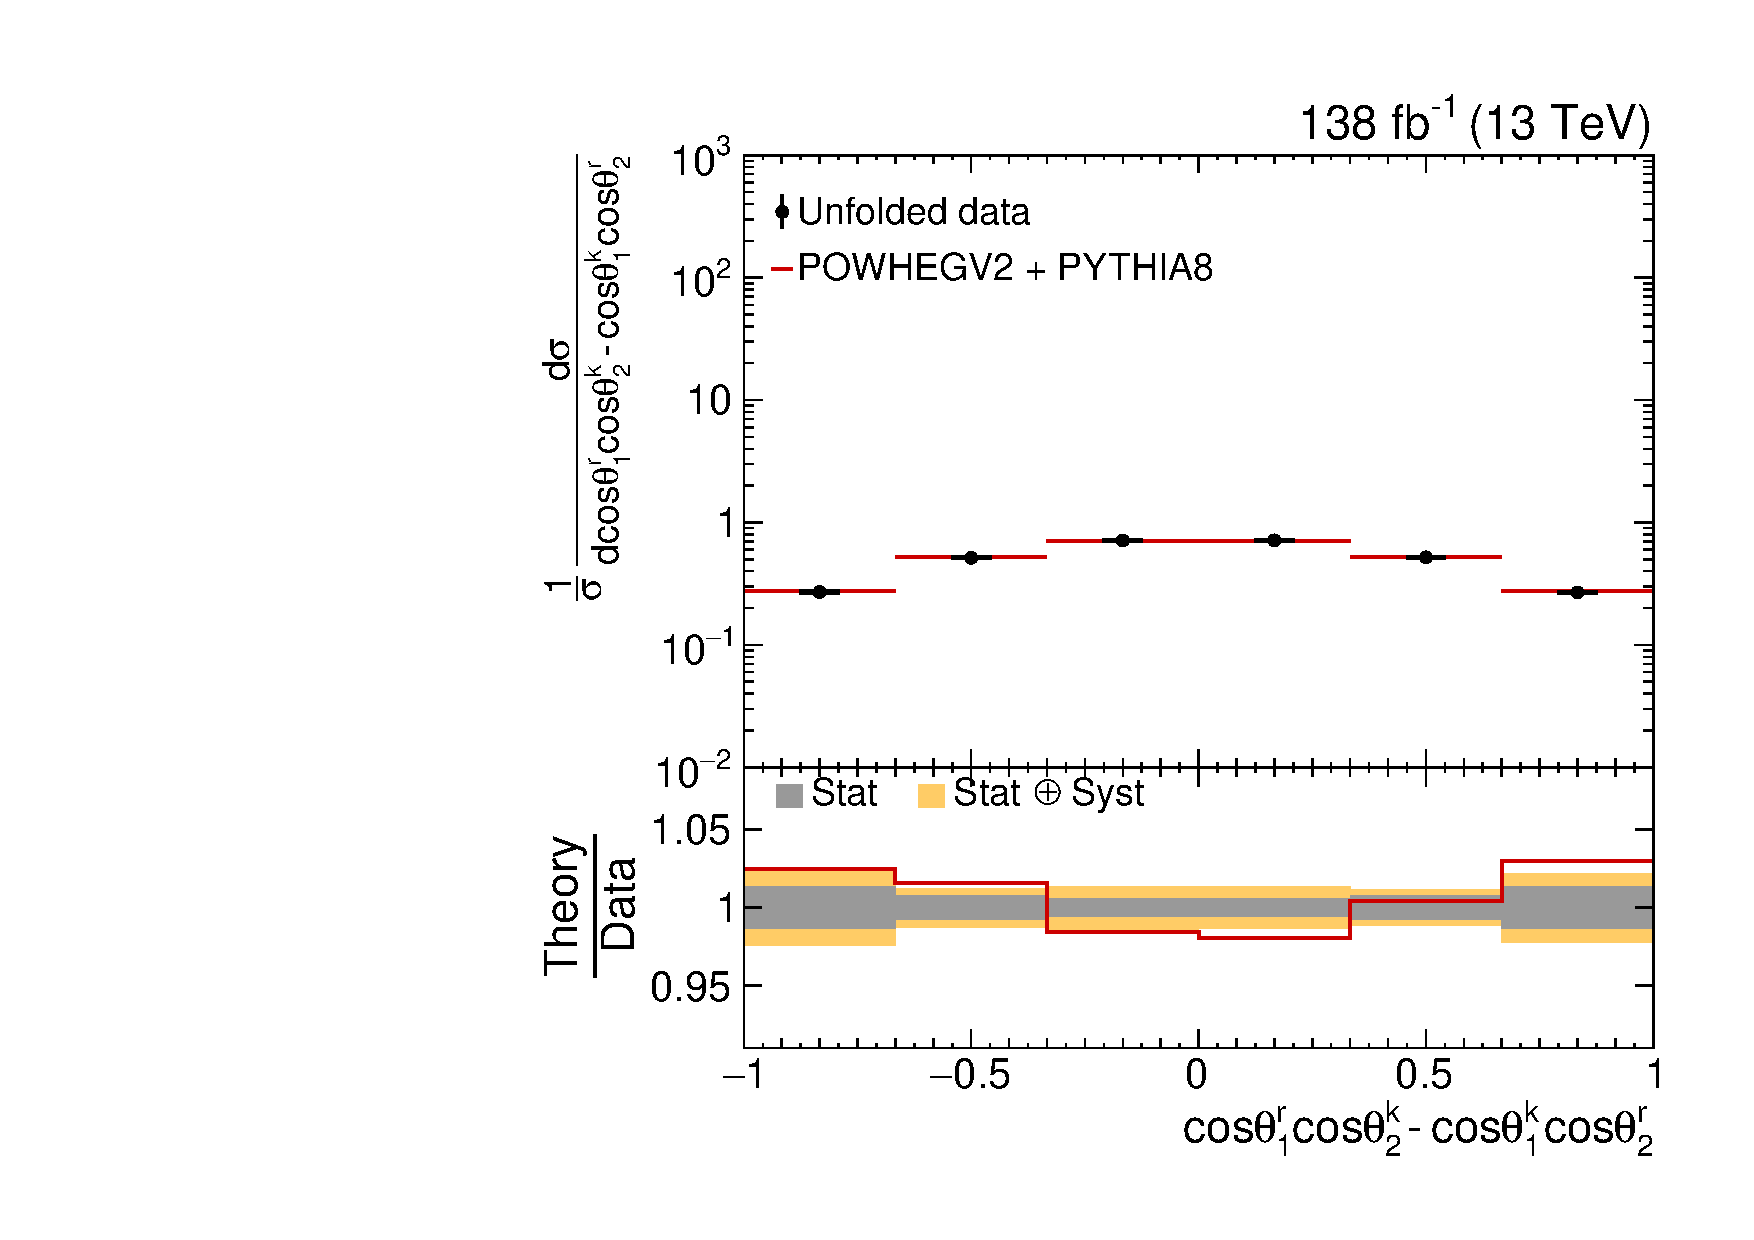
\includegraphics[width=0.40\textwidth]{fig_fullRun2UL/unfolding/combined/UnfoldedResultsNorm_c_Mrk.pdf} \\
\label{fig:c_Mrk}
\caption{Reconstructed detector-level distribution (Top Left), detector response-matrix (Top Right), absolute cross-section unfolded to parton-level (Bottom Left), and normalized cross-section unfolded to parton-level (Bottom Right) for off-diagonal spin correlation difference observable $\cos\theta_{1}^{r}\cos\theta_{2}^{k}-\cos\theta_{1}^{k}\cos\theta_{2}^{r}$, from which spin-density coefficient $C_{rk}-C_{kr}$ (sensitive to spin-density coefficient function $c_n$) is extracted.}
\end{center}
\end{figure}
\clearpage
\begin{figure}[htb]
\begin{center}
 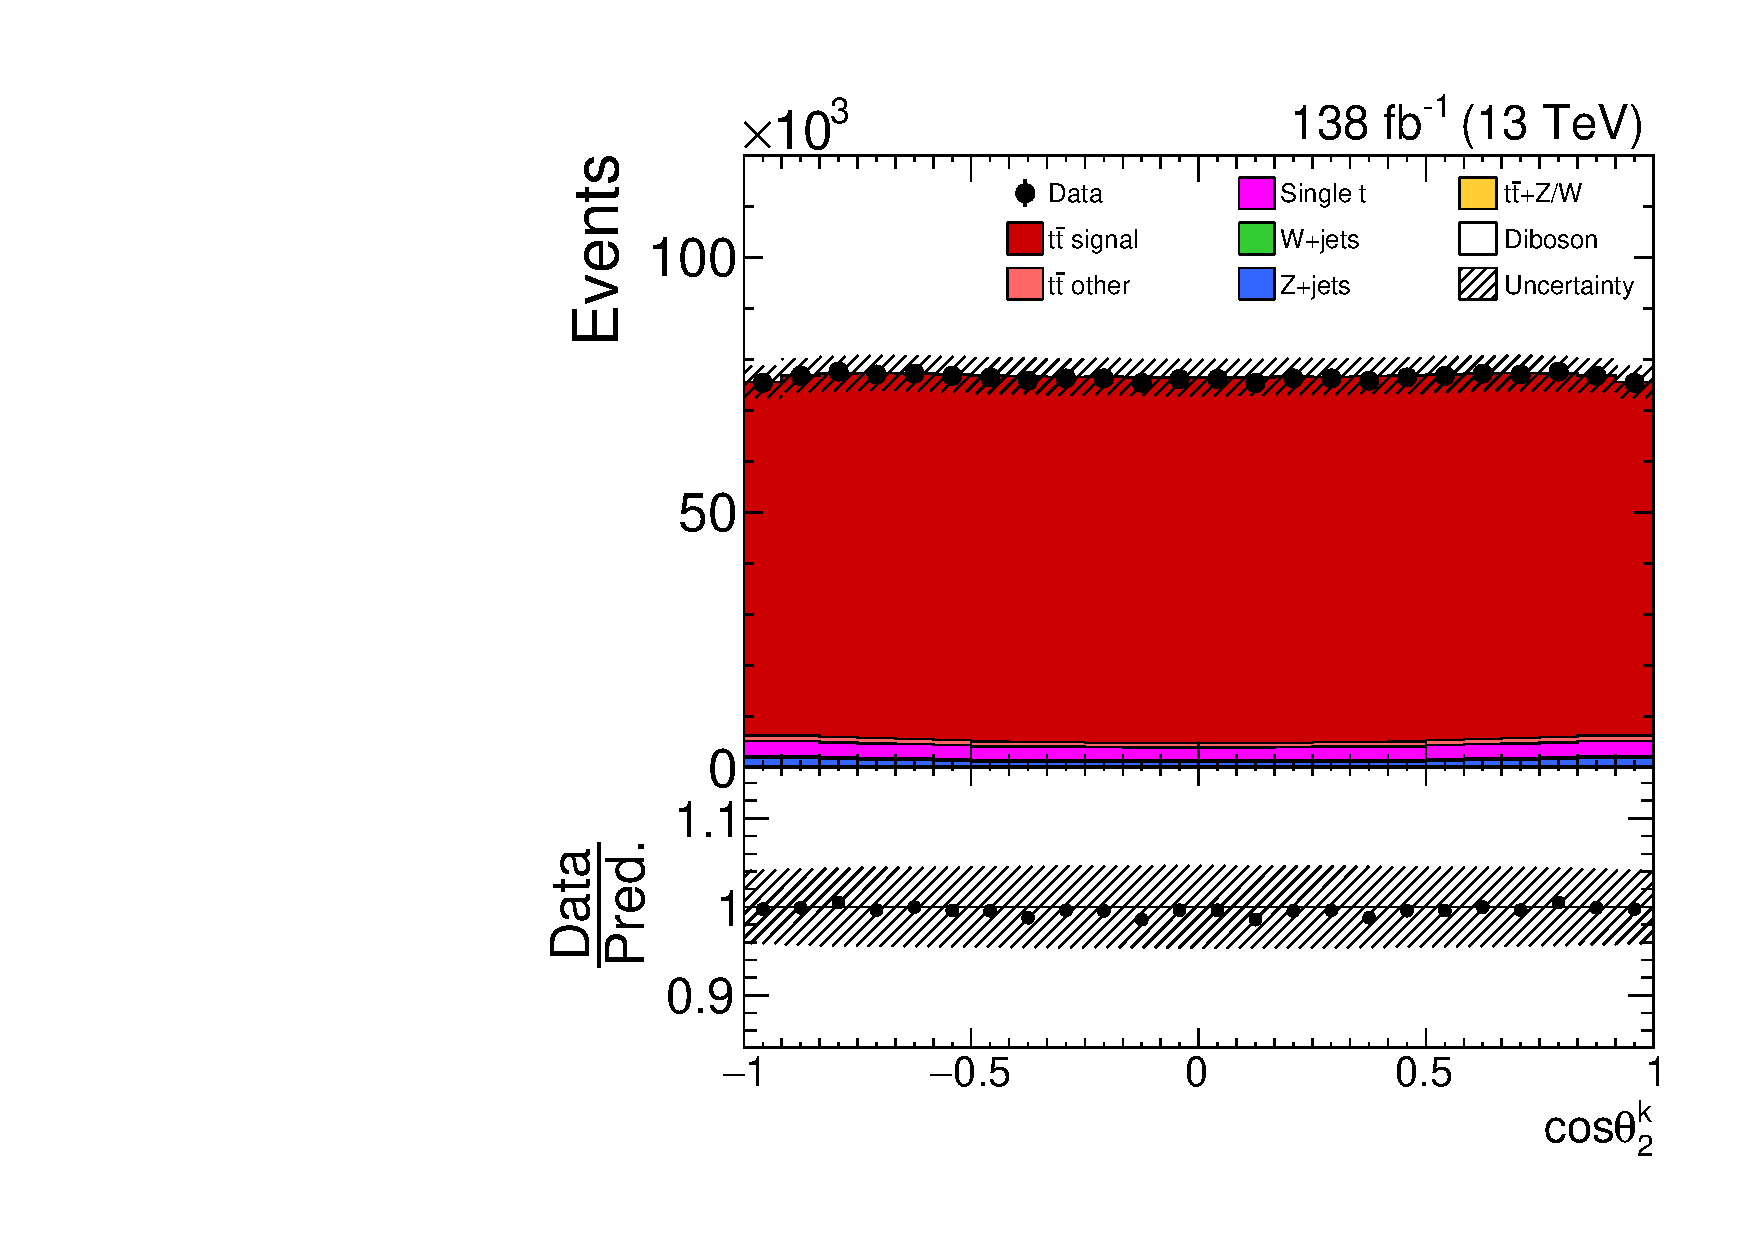
\includegraphics[width=0.40\textwidth]{fig_fullRun2UL/controlplots/combined/Hyp_LeptonBk.pdf}
 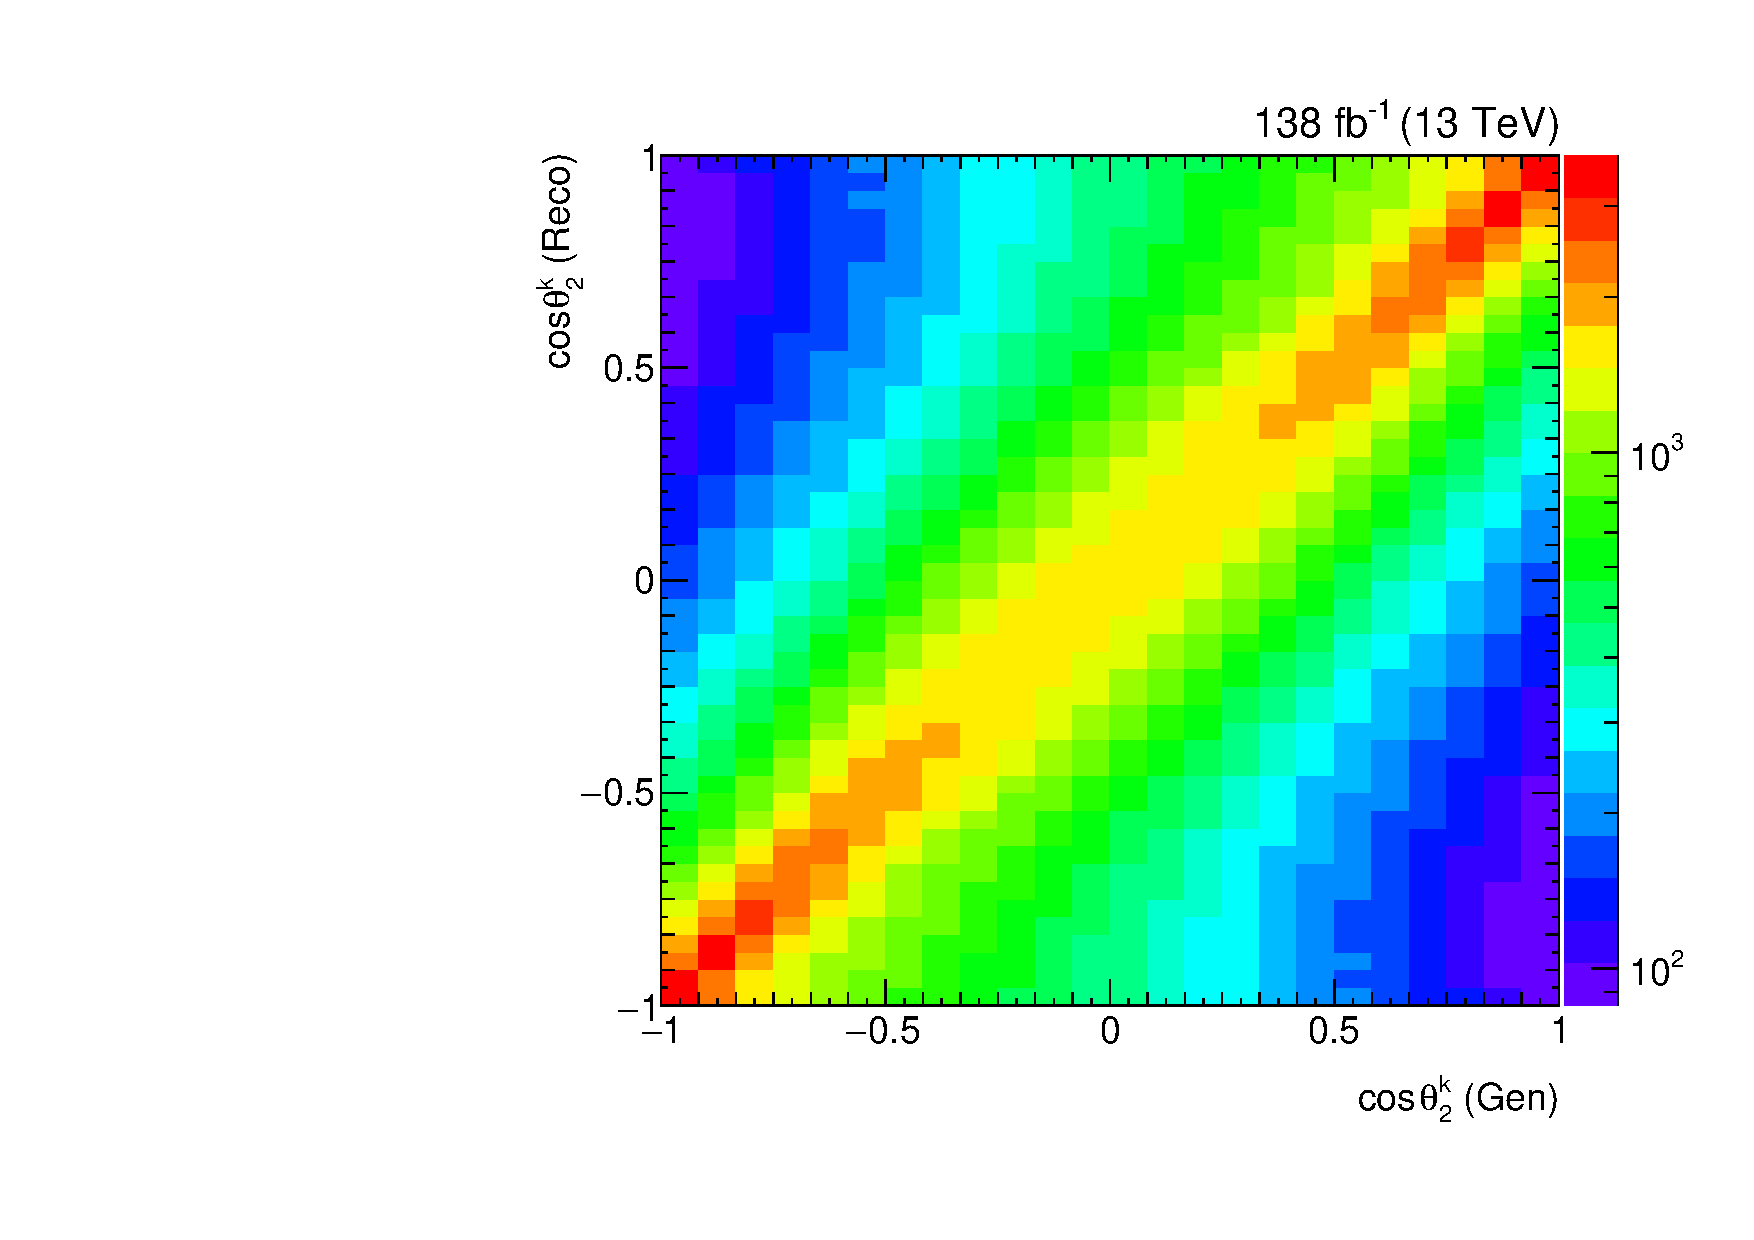
\includegraphics[width=0.40\textwidth]{fig_fullRun2UL/unfolding/combined/ResponseMatrix_b2k.pdf} \\
 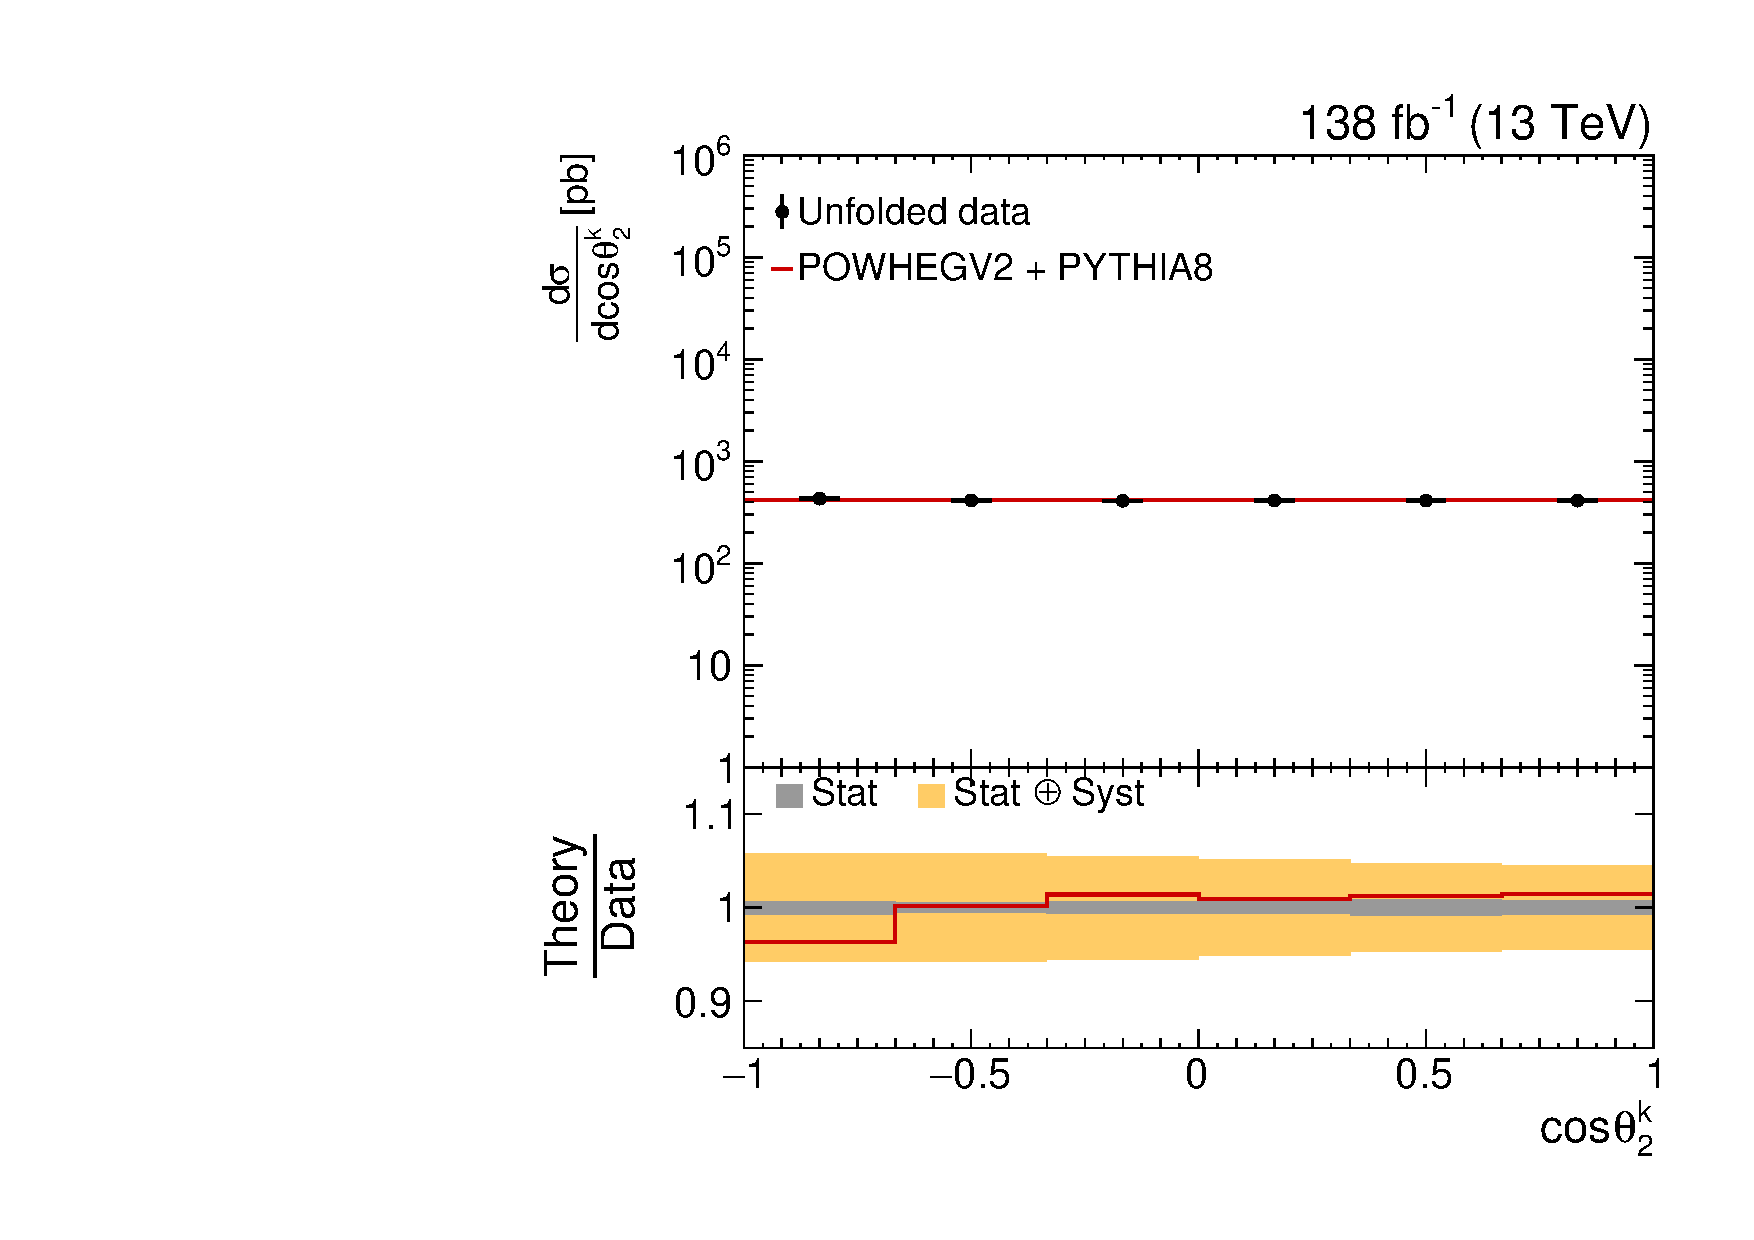
\includegraphics[width=0.40\textwidth]{fig_fullRun2UL/unfolding/combined/UnfoldedResults_b2k.pdf}
 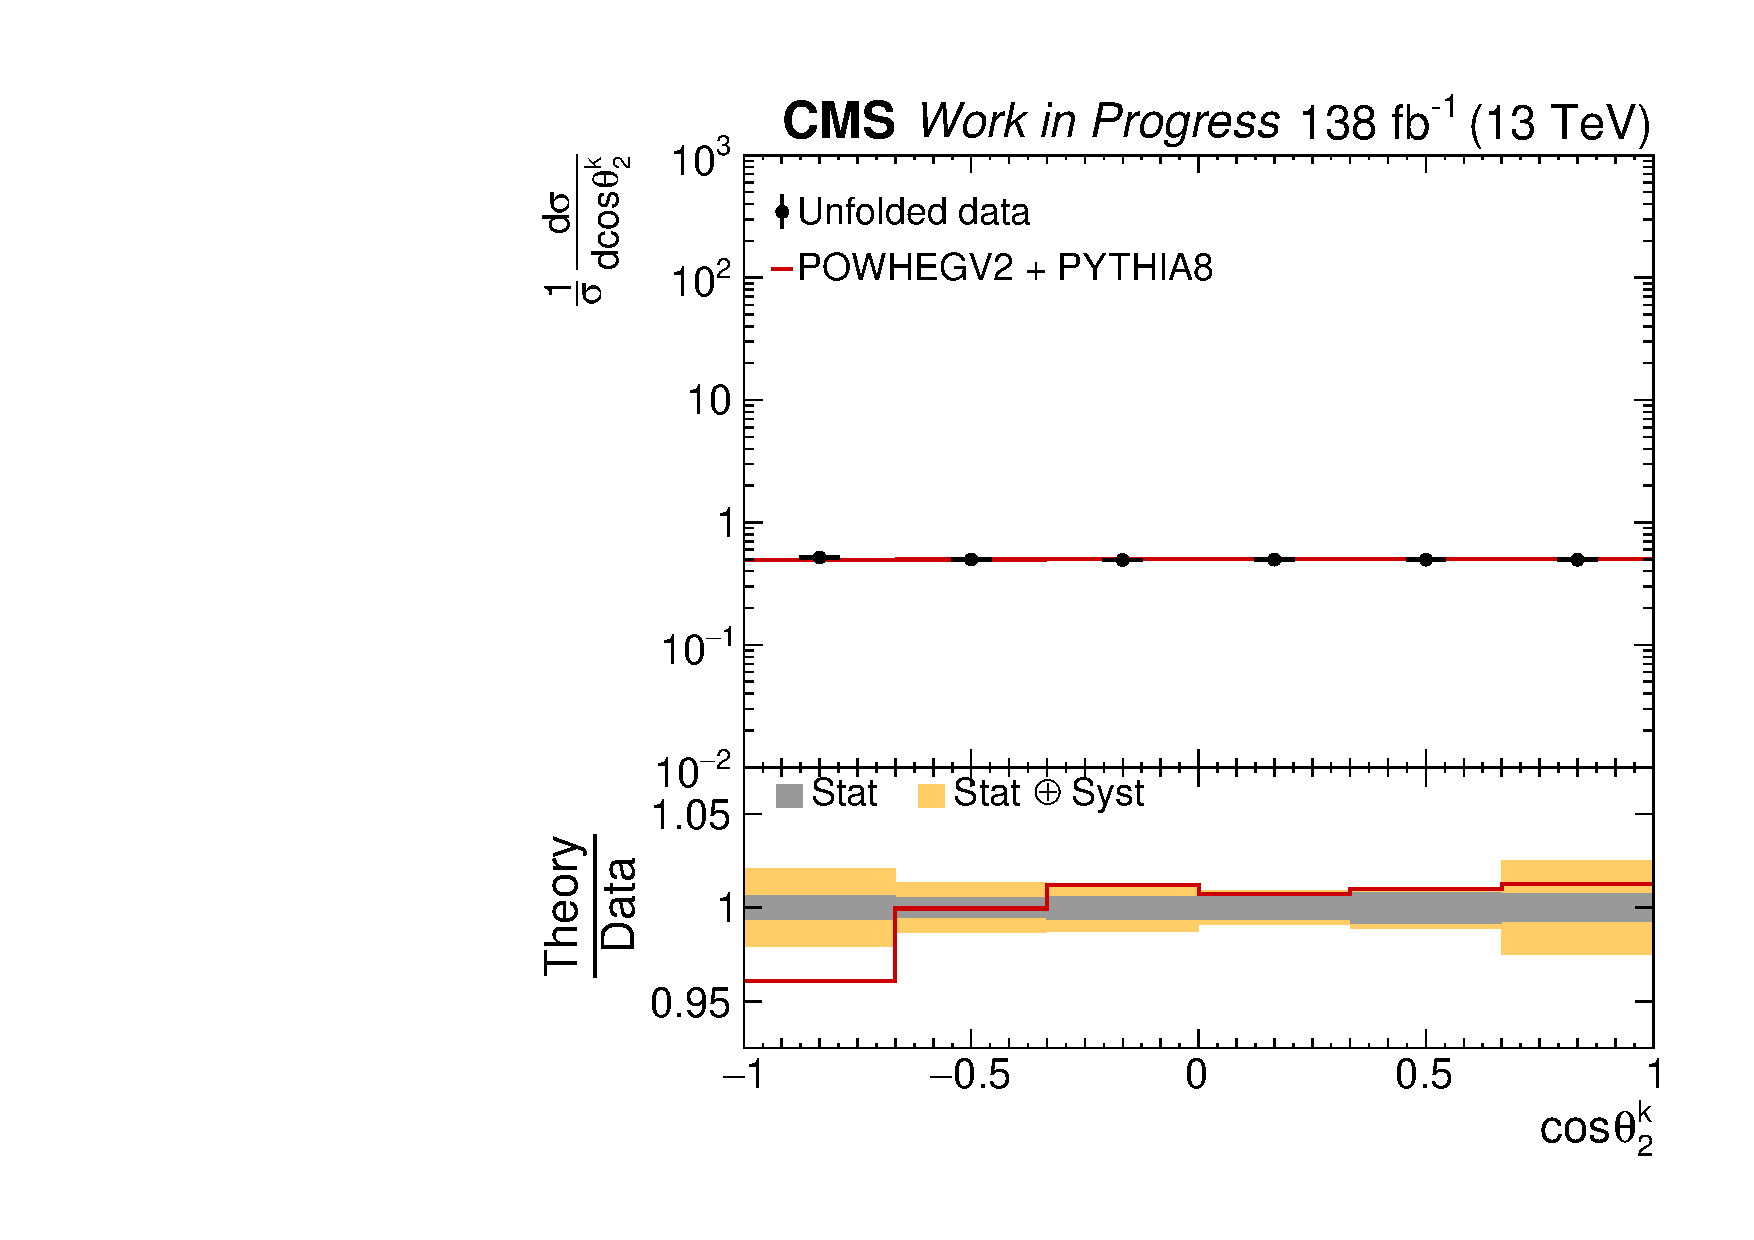
\includegraphics[width=0.40\textwidth]{fig_fullRun2UL/unfolding/combined/UnfoldedResultsNorm_b2k.pdf} \\
\label{fig:b2k}
\caption{Reconstructed detector-level distribution (Top Left), detector response-matrix (Top Right), absolute cross-section unfolded to parton-level (Bottom Left), and normalized cross-section unfolded to parton-level (Bottom Right) for polarization observable $\cos\theta_{2}^{k}$, from which spin-density coefficient $B_{2}^{k}$ (sensitive to spin-density coefficient function $b_k^{-}$) is extracted.}
\end{center}
\end{figure}
\clearpage
\begin{figure}[htb]
\begin{center}
 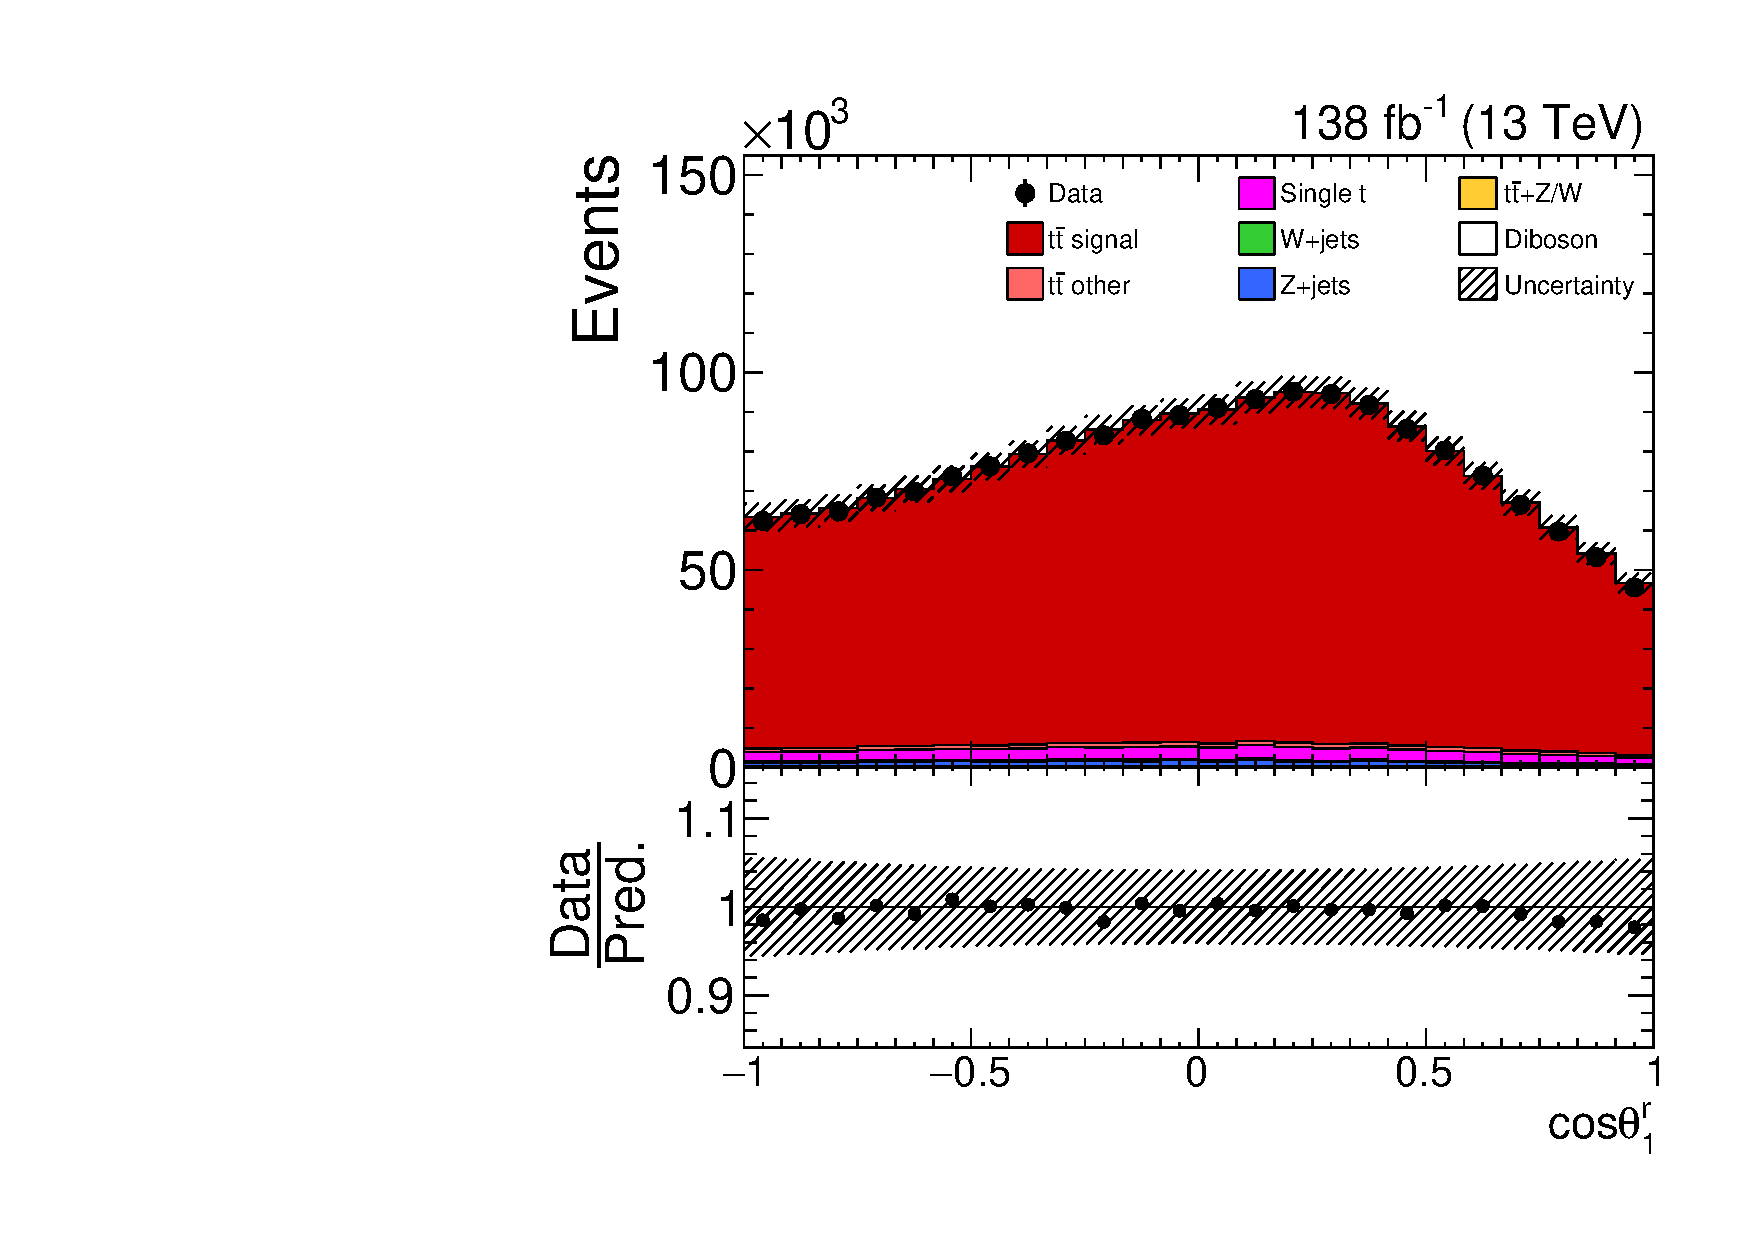
\includegraphics[width=0.40\textwidth]{fig_fullRun2UL/controlplots/combined/Hyp_AntiLeptonBr.pdf}
 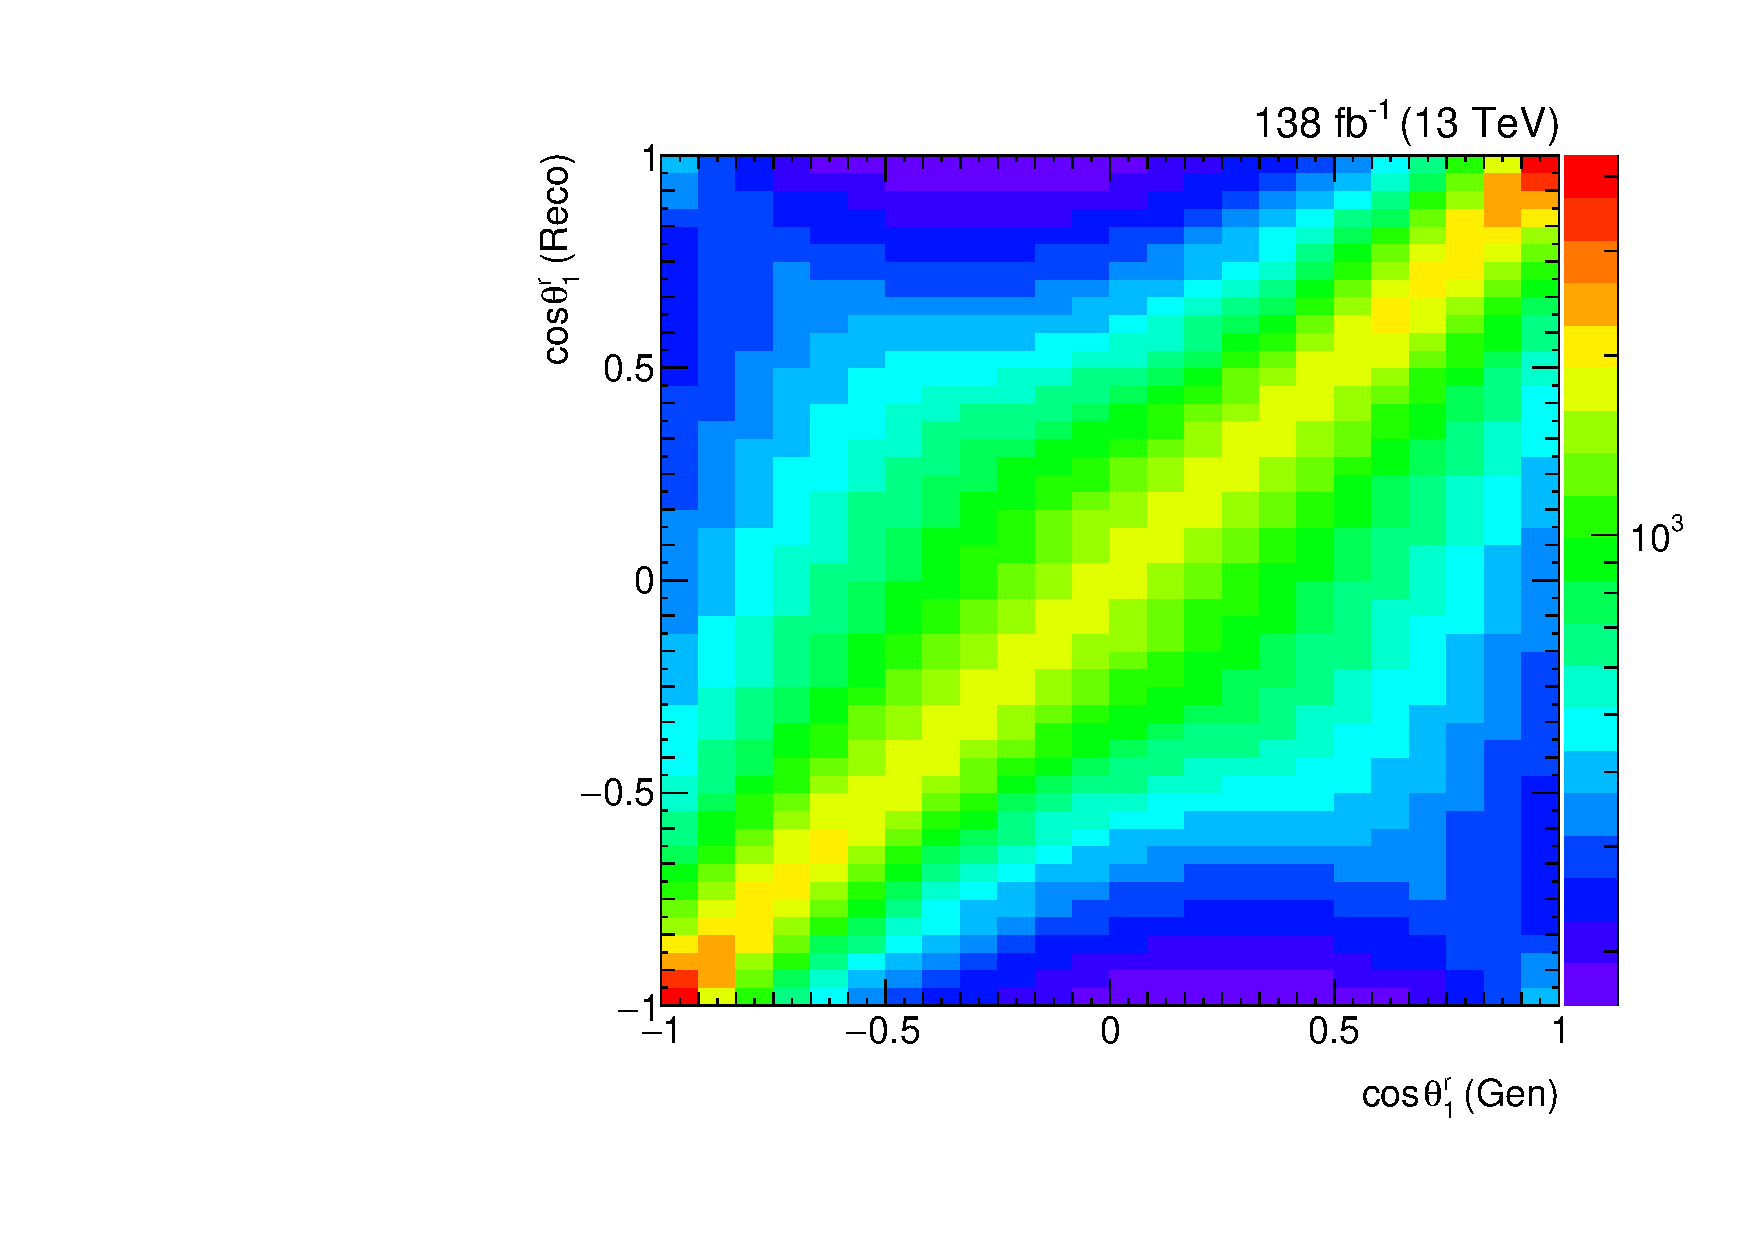
\includegraphics[width=0.40\textwidth]{fig_fullRun2UL/unfolding/combined/ResponseMatrix_b1r.pdf} \\
 \includegraphics[width=0.40\textwidth]{fig_fullRun2UL/unfolding/combined/UnfoldedResults_b1r.pdf}
 \includegraphics[width=0.40\textwidth]{fig_fullRun2UL/unfolding/combined/UnfoldedResultsNorm_b1r.pdf} \\
\label{fig:b1r}
\caption{Reconstructed detector-level distribution (Top Left), detector response-matrix (Top Right), absolute cross-section unfolded to parton-level (Bottom Left), and normalized cross-section unfolded to parton-level (Bottom Right) for polarization observable $\cos\theta_{1}^{r}$, from which spin-density coefficient $B_{1}^{r}$ (sensitive to spin-density coefficient function $b_r^{+}$) is extracted.}
\end{center}
\end{figure}
\clearpage
\begin{figure}[htb]
\begin{center}
 \includegraphics[width=0.40\textwidth]{fig_fullRun2UL/controlplots/combined/Hyp_LLBarcHel.pdf}
 \includegraphics[width=0.40\textwidth]{fig_fullRun2UL/unfolding/combined/ResponseMatrix_ll_cHel.pdf} \\
 \includegraphics[width=0.40\textwidth]{fig_fullRun2UL/unfolding/combined/UnfoldedResults_ll_cHel.pdf}
 \includegraphics[width=0.40\textwidth]{fig_fullRun2UL/unfolding/combined/UnfoldedResultsNorm_ll_cHel.pdf} \\
\label{fig:ll_cHel}
\caption{Reconstructed detector-level distribution (Top Left), detector response-matrix (Top Right), absolute cross-section unfolded to parton-level (Bottom Left), and normalized cross-section unfolded to parton-level (Bottom Right) for  observable $\cos\varphi$, from which spin-density coefficient $D = -frac{1}{3}(C_{kk} + C_{rr} + C_{nn})$ (sensitive to spin-density coefficient function $-frac{1}{3}(c_{kk} + c_{rr} + c_{nn})$) is extracted.}
\end{center}
\end{figure}
\clearpage
\begin{figure}[htb]
\begin{center}
 \includegraphics[width=0.40\textwidth]{fig_fullRun2UL/controlplots/combined/Hyp_LLBarCMnr.pdf}
 \includegraphics[width=0.40\textwidth]{fig_fullRun2UL/unfolding/combined/ResponseMatrix_c_Mnr.pdf} \\
 \includegraphics[width=0.40\textwidth]{fig_fullRun2UL/unfolding/combined/UnfoldedResults_c_Mnr.pdf}
 \includegraphics[width=0.40\textwidth]{fig_fullRun2UL/unfolding/combined/UnfoldedResultsNorm_c_Mnr.pdf} \\
\label{fig:c_Mnr}
\caption{Reconstructed detector-level distribution (Top Left), detector response-matrix (Top Right), absolute cross-section unfolded to parton-level (Bottom Left), and normalized cross-section unfolded to parton-level (Bottom Right) for off-diagonal spin correlation difference observable $\cos\theta_{1}^{n}\cos\theta_{2}^{r}-\cos\theta_{1}^{r}\cos\theta_{2}^{n}$, from which spin-density coefficient $C_{nr}-C_{rn}$ (sensitive to spin-density coefficient function $c_k$) is extracted.}
\end{center}
\end{figure}
\clearpage
\begin{figure}[htb]
\begin{center}
 \includegraphics[width=0.40\textwidth]{fig_fullRun2UL/controlplots/combined/Hyp_LLBarCPnr.pdf}
 \includegraphics[width=0.40\textwidth]{fig_fullRun2UL/unfolding/combined/ResponseMatrix_c_Pnr.pdf} \\
 \includegraphics[width=0.40\textwidth]{fig_fullRun2UL/unfolding/combined/UnfoldedResults_c_Pnr.pdf}
 \includegraphics[width=0.40\textwidth]{fig_fullRun2UL/unfolding/combined/UnfoldedResultsNorm_c_Pnr.pdf} \\
\label{fig:c_Pnr}
\caption{Reconstructed detector-level distribution (Top Left), detector response-matrix (Top Right), absolute cross-section unfolded to parton-level (Bottom Left), and normalized cross-section unfolded to parton-level (Bottom Right) for off-diagonal spin correlation sum observable $\cos\theta_{1}^{n}\cos\theta_{2}^{r}+\cos\theta_{1}^{r}\cos\theta_{2}^{n}$, from which spin-density coefficient $C_{nr}+C_{rn}$ (sensitive to spin-density coefficient function $c_{n r}$) is extracted.}
\end{center}
\end{figure}
\clearpage
\begin{figure}[htb]
\begin{center}
 \includegraphics[width=0.40\textwidth]{fig_fullRun2UL/controlplots/combined/Hyp_LLBarCkk_vs_TTBarMass.pdf}
 \includegraphics[width=0.40\textwidth]{fig_fullRun2UL/unfolding/combined/ResponseMatrix_c_kk_mttbar.pdf} \\
 \includegraphics[width=0.40\textwidth]{fig_fullRun2UL/unfolding/combined/UnfoldedResults_c_kk_mttbar.pdf}
 \includegraphics[width=0.40\textwidth]{fig_fullRun2UL/unfolding/combined/UnfoldedResultsNorm_c_kk_mttbar.pdf} \\
\label{fig:c_kk_mttbar}
\caption{Differential reconstructed detector-level distributions (Top Left), detector response-matrices (Top Right), absolute cross-sections unfolded to parton-level (Bottom Left), and normalized cross-sections unfolded to parton-level (Bottom Right) for diagonal spin correlation observable $\cos\theta_{1}^{k}\cos\theta_{2}^{k}$ as a function of $m_{t\bar{t}}$, from which spin-density coefficient $C_{kk}$ (sensitive to spin-density coefficient function $c_{k k}$) is extracted.}
\end{center}
\end{figure}
\clearpage
\begin{figure}[htb]
\begin{center}
 \includegraphics[width=0.40\textwidth]{fig_fullRun2UL/controlplots/combined/Hyp_LLBarCPrk_vs_TTBarMass.pdf}
 \includegraphics[width=0.40\textwidth]{fig_fullRun2UL/unfolding/combined/ResponseMatrix_c_Prk_mttbar.pdf} \\
 \includegraphics[width=0.40\textwidth]{fig_fullRun2UL/unfolding/combined/UnfoldedResults_c_Prk_mttbar.pdf}
 \includegraphics[width=0.40\textwidth]{fig_fullRun2UL/unfolding/combined/UnfoldedResultsNorm_c_Prk_mttbar.pdf} \\
\label{fig:c_Prk_mttbar}
\caption{Differential reconstructed detector-level distributions (Top Left), detector response-matrices (Top Right), absolute cross-sections unfolded to parton-level (Bottom Left), and normalized cross-sections unfolded to parton-level (Bottom Right) for off-diagonal spin correlation sum observable $\cos\theta_{1}^{r}\cos\theta_{2}^{k}+\cos\theta_{1}^{k}\cos\theta_{2}^{r}$ as a function of $m_{t\bar{t}}$, from which spin-density coefficient $C_{rk}+C_{kr}$ (sensitive to spin-density coefficient function $c_{r k}$) is extracted.}
\end{center}
\end{figure}
\clearpage
\begin{figure}[htb]
\begin{center}
 \includegraphics[width=0.40\textwidth]{fig_fullRun2UL/controlplots/combined/Hyp_LLBarCPnk_vs_TTBarMass.pdf}
 \includegraphics[width=0.40\textwidth]{fig_fullRun2UL/unfolding/combined/ResponseMatrix_c_Pnk_mttbar.pdf} \\
 \includegraphics[width=0.40\textwidth]{fig_fullRun2UL/unfolding/combined/UnfoldedResults_c_Pnk_mttbar.pdf}
 \includegraphics[width=0.40\textwidth]{fig_fullRun2UL/unfolding/combined/UnfoldedResultsNorm_c_Pnk_mttbar.pdf} \\
\label{fig:c_Pnk_mttbar}
\caption{Differential reconstructed detector-level distributions (Top Left), detector response-matrices (Top Right), absolute cross-sections unfolded to parton-level (Bottom Left), and normalized cross-sections unfolded to parton-level (Bottom Right) for off-diagonal spin correlation sum observable $\cos\theta_{1}^{n}\cos\theta_{2}^{k}+\cos\theta_{1}^{k}\cos\theta_{2}^{n}$ as a function of $m_{t\bar{t}}$, from which spin-density coefficient $C_{nk}+C_{kn}$ (sensitive to spin-density coefficient function $c_{k n}$) is extracted.}
\end{center}
\end{figure}
\clearpage
\begin{figure}[htb]
\begin{center}
 \includegraphics[width=0.40\textwidth]{fig_fullRun2UL/controlplots/combined/Hyp_LLBarCrr_vs_TTBarMass.pdf}
 \includegraphics[width=0.40\textwidth]{fig_fullRun2UL/unfolding/combined/ResponseMatrix_c_rr_mttbar.pdf} \\
 \includegraphics[width=0.40\textwidth]{fig_fullRun2UL/unfolding/combined/UnfoldedResults_c_rr_mttbar.pdf}
 \includegraphics[width=0.40\textwidth]{fig_fullRun2UL/unfolding/combined/UnfoldedResultsNorm_c_rr_mttbar.pdf} \\
\label{fig:c_rr_mttbar}
\caption{Differential reconstructed detector-level distributions (Top Left), detector response-matrices (Top Right), absolute cross-sections unfolded to parton-level (Bottom Left), and normalized cross-sections unfolded to parton-level (Bottom Right) for diagonal spin correlation observable $\cos\theta_{1}^{r}\cos\theta_{2}^{r}$ as a function of $m_{t\bar{t}}$, from which spin-density coefficient $C_{rr}$ (sensitive to spin-density coefficient function $c_{r r}$) is extracted.}
\end{center}
\end{figure}
\clearpage
\begin{figure}[htb]
\begin{center}
 \includegraphics[width=0.40\textwidth]{fig_fullRun2UL/controlplots/combined/Hyp_LLBarCMnk_vs_TTBarMass.pdf}
 \includegraphics[width=0.40\textwidth]{fig_fullRun2UL/unfolding/combined/ResponseMatrix_c_Mnk_mttbar.pdf} \\
 \includegraphics[width=0.40\textwidth]{fig_fullRun2UL/unfolding/combined/UnfoldedResults_c_Mnk_mttbar.pdf}
 \includegraphics[width=0.40\textwidth]{fig_fullRun2UL/unfolding/combined/UnfoldedResultsNorm_c_Mnk_mttbar.pdf} \\
\label{fig:c_Mnk_mttbar}
\caption{Differential reconstructed detector-level distributions (Top Left), detector response-matrices (Top Right), absolute cross-sections unfolded to parton-level (Bottom Left), and normalized cross-sections unfolded to parton-level (Bottom Right) for off-diagonal spin correlation difference observable $\cos\theta_{1}^{n}\cos\theta_{2}^{k}-\cos\theta_{1}^{k}\cos\theta_{2}^{n}$ as a function of $m_{t\bar{t}}$, from which spin-density coefficient $C_{nk}-C_{kn}$ (sensitive to spin-density coefficient function $-c_r$) is extracted.}
\end{center}
\end{figure}
\clearpage
\begin{figure}[htb]
\begin{center}
 \includegraphics[width=0.40\textwidth]{fig_fullRun2UL/controlplots/combined/Hyp_AntiLeptonBn_vs_TTBarMass.pdf}
 \includegraphics[width=0.40\textwidth]{fig_fullRun2UL/unfolding/combined/ResponseMatrix_b1n_mttbar.pdf} \\
 \includegraphics[width=0.40\textwidth]{fig_fullRun2UL/unfolding/combined/UnfoldedResults_b1n_mttbar.pdf}
 \includegraphics[width=0.40\textwidth]{fig_fullRun2UL/unfolding/combined/UnfoldedResultsNorm_b1n_mttbar.pdf} \\
\label{fig:b1n_mttbar}
\caption{Differential reconstructed detector-level distributions (Top Left), detector response-matrices (Top Right), absolute cross-sections unfolded to parton-level (Bottom Left), and normalized cross-sections unfolded to parton-level (Bottom Right) for polarization observable $\cos\theta_{1}^{n}$ as a function of $m_{t\bar{t}}$, from which spin-density coefficient $B_{1}^{n}$ (sensitive to spin-density coefficient function $b_n^{+}$) is extracted.}
\end{center}
\end{figure}
\clearpage
\begin{figure}[htb]
\begin{center}
 \includegraphics[width=0.40\textwidth]{fig_fullRun2UL/controlplots/combined/Hyp_AntiLeptonBk_vs_TTBarMass.pdf}
 \includegraphics[width=0.40\textwidth]{fig_fullRun2UL/unfolding/combined/ResponseMatrix_b1k_mttbar.pdf} \\
 \includegraphics[width=0.40\textwidth]{fig_fullRun2UL/unfolding/combined/UnfoldedResults_b1k_mttbar.pdf}
 \includegraphics[width=0.40\textwidth]{fig_fullRun2UL/unfolding/combined/UnfoldedResultsNorm_b1k_mttbar.pdf} \\
\label{fig:b1k_mttbar}
\caption{Differential reconstructed detector-level distributions (Top Left), detector response-matrices (Top Right), absolute cross-sections unfolded to parton-level (Bottom Left), and normalized cross-sections unfolded to parton-level (Bottom Right) for polarization observable $\cos\theta_{1}^{k}$ as a function of $m_{t\bar{t}}$, from which spin-density coefficient $B_{1}^{k}$ (sensitive to spin-density coefficient function $b_k^{+}$) is extracted.}
\end{center}
\end{figure}
\clearpage
\begin{figure}[htb]
\begin{center}
 \includegraphics[width=0.40\textwidth]{fig_fullRun2UL/controlplots/combined/Hyp_LLBarCnn_vs_TTBarMass.pdf}
 \includegraphics[width=0.40\textwidth]{fig_fullRun2UL/unfolding/combined/ResponseMatrix_c_nn_mttbar.pdf} \\
 \includegraphics[width=0.40\textwidth]{fig_fullRun2UL/unfolding/combined/UnfoldedResults_c_nn_mttbar.pdf}
 \includegraphics[width=0.40\textwidth]{fig_fullRun2UL/unfolding/combined/UnfoldedResultsNorm_c_nn_mttbar.pdf} \\
\label{fig:c_nn_mttbar}
\caption{Differential reconstructed detector-level distributions (Top Left), detector response-matrices (Top Right), absolute cross-sections unfolded to parton-level (Bottom Left), and normalized cross-sections unfolded to parton-level (Bottom Right) for diagonal spin correlation observable $\cos\theta_{1}^{n}\cos\theta_{2}^{n}$ as a function of $m_{t\bar{t}}$, from which spin-density coefficient $C_{nn}$ (sensitive to spin-density coefficient function $c_{n n}$) is extracted.}
\end{center}
\end{figure}
\clearpage
\begin{figure}[htb]
\begin{center}
 \includegraphics[width=0.40\textwidth]{fig_fullRun2UL/controlplots/combined/Hyp_LeptonBr_vs_TTBarMass.pdf}
 \includegraphics[width=0.40\textwidth]{fig_fullRun2UL/unfolding/combined/ResponseMatrix_b2r_mttbar.pdf} \\
 \includegraphics[width=0.40\textwidth]{fig_fullRun2UL/unfolding/combined/UnfoldedResults_b2r_mttbar.pdf}
 \includegraphics[width=0.40\textwidth]{fig_fullRun2UL/unfolding/combined/UnfoldedResultsNorm_b2r_mttbar.pdf} \\
\label{fig:b2r_mttbar}
\caption{Differential reconstructed detector-level distributions (Top Left), detector response-matrices (Top Right), absolute cross-sections unfolded to parton-level (Bottom Left), and normalized cross-sections unfolded to parton-level (Bottom Right) for polarization observable $\cos\theta_{2}^{r}$ as a function of $m_{t\bar{t}}$, from which spin-density coefficient $B_{2}^{r}$ (sensitive to spin-density coefficient function $b_r^{-}$) is extracted.}
\end{center}
\end{figure}
\clearpage
\begin{figure}[htb]
\begin{center}
 \includegraphics[width=0.40\textwidth]{fig_fullRun2UL/controlplots/combined/Hyp_LeptonBn_vs_TTBarMass.pdf}
 \includegraphics[width=0.40\textwidth]{fig_fullRun2UL/unfolding/combined/ResponseMatrix_b2n_mttbar.pdf} \\
 \includegraphics[width=0.40\textwidth]{fig_fullRun2UL/unfolding/combined/UnfoldedResults_b2n_mttbar.pdf}
 \includegraphics[width=0.40\textwidth]{fig_fullRun2UL/unfolding/combined/UnfoldedResultsNorm_b2n_mttbar.pdf} \\
\label{fig:b2n_mttbar}
\caption{Differential reconstructed detector-level distributions (Top Left), detector response-matrices (Top Right), absolute cross-sections unfolded to parton-level (Bottom Left), and normalized cross-sections unfolded to parton-level (Bottom Right) for polarization observable $\cos\theta_{2}^{n}$ as a function of $m_{t\bar{t}}$, from which spin-density coefficient $B_{2}^{n}$ (sensitive to spin-density coefficient function $b_n^{-}$) is extracted.}
\end{center}
\end{figure}
\clearpage
\begin{figure}[htb]
\begin{center}
 \includegraphics[width=0.40\textwidth]{fig_fullRun2UL/controlplots/combined/Hyp_LLBarCMrk_vs_TTBarMass.pdf}
 \includegraphics[width=0.40\textwidth]{fig_fullRun2UL/unfolding/combined/ResponseMatrix_c_Mrk_mttbar.pdf} \\
 \includegraphics[width=0.40\textwidth]{fig_fullRun2UL/unfolding/combined/UnfoldedResults_c_Mrk_mttbar.pdf}
 \includegraphics[width=0.40\textwidth]{fig_fullRun2UL/unfolding/combined/UnfoldedResultsNorm_c_Mrk_mttbar.pdf} \\
\label{fig:c_Mrk_mttbar}
\caption{Differential reconstructed detector-level distributions (Top Left), detector response-matrices (Top Right), absolute cross-sections unfolded to parton-level (Bottom Left), and normalized cross-sections unfolded to parton-level (Bottom Right) for off-diagonal spin correlation difference observable $\cos\theta_{1}^{r}\cos\theta_{2}^{k}-\cos\theta_{1}^{k}\cos\theta_{2}^{r}$ as a function of $m_{t\bar{t}}$, from which spin-density coefficient $C_{rk}-C_{kr}$ (sensitive to spin-density coefficient function $c_n$) is extracted.}
\end{center}
\end{figure}
\clearpage
\begin{figure}[htb]
\begin{center}
 \includegraphics[width=0.40\textwidth]{fig_fullRun2UL/controlplots/combined/Hyp_LeptonBk_vs_TTBarMass.pdf}
 \includegraphics[width=0.40\textwidth]{fig_fullRun2UL/unfolding/combined/ResponseMatrix_b2k_mttbar.pdf} \\
 \includegraphics[width=0.40\textwidth]{fig_fullRun2UL/unfolding/combined/UnfoldedResults_b2k_mttbar.pdf}
 \includegraphics[width=0.40\textwidth]{fig_fullRun2UL/unfolding/combined/UnfoldedResultsNorm_b2k_mttbar.pdf} \\
\label{fig:b2k_mttbar}
\caption{Differential reconstructed detector-level distributions (Top Left), detector response-matrices (Top Right), absolute cross-sections unfolded to parton-level (Bottom Left), and normalized cross-sections unfolded to parton-level (Bottom Right) for polarization observable $\cos\theta_{2}^{k}$ as a function of $m_{t\bar{t}}$, from which spin-density coefficient $B_{2}^{k}$ (sensitive to spin-density coefficient function $b_k^{-}$) is extracted.}
\end{center}
\end{figure}
\clearpage
\begin{figure}[htb]
\begin{center}
 \includegraphics[width=0.40\textwidth]{fig_fullRun2UL/controlplots/combined/Hyp_AntiLeptonBr_vs_TTBarMass.pdf}
 \includegraphics[width=0.40\textwidth]{fig_fullRun2UL/unfolding/combined/ResponseMatrix_b1r_mttbar.pdf} \\
 \includegraphics[width=0.40\textwidth]{fig_fullRun2UL/unfolding/combined/UnfoldedResults_b1r_mttbar.pdf}
 \includegraphics[width=0.40\textwidth]{fig_fullRun2UL/unfolding/combined/UnfoldedResultsNorm_b1r_mttbar.pdf} \\
\label{fig:b1r_mttbar}
\caption{Differential reconstructed detector-level distributions (Top Left), detector response-matrices (Top Right), absolute cross-sections unfolded to parton-level (Bottom Left), and normalized cross-sections unfolded to parton-level (Bottom Right) for polarization observable $\cos\theta_{1}^{r}$ as a function of $m_{t\bar{t}}$, from which spin-density coefficient $B_{1}^{r}$ (sensitive to spin-density coefficient function $b_r^{+}$) is extracted.}
\end{center}
\end{figure}
\clearpage
\begin{figure}[htb]
\begin{center}
 \includegraphics[width=0.40\textwidth]{fig_fullRun2UL/controlplots/combined/Hyp_LLBarcHel_vs_TTBarMass.pdf}
 \includegraphics[width=0.40\textwidth]{fig_fullRun2UL/unfolding/combined/ResponseMatrix_ll_cHel_mttbar.pdf} \\
 \includegraphics[width=0.40\textwidth]{fig_fullRun2UL/unfolding/combined/UnfoldedResults_ll_cHel_mttbar.pdf}
 \includegraphics[width=0.40\textwidth]{fig_fullRun2UL/unfolding/combined/UnfoldedResultsNorm_ll_cHel_mttbar.pdf} \\
\label{fig:ll_cHel_mttbar}
\caption{Differential reconstructed detector-level distributions (Top Left), detector response-matrices (Top Right), absolute cross-sections unfolded to parton-level (Bottom Left), and normalized cross-sections unfolded to parton-level (Bottom Right) for  observable $\cos\varphi$ as a function of $m_{t\bar{t}}$, from which spin-density coefficient $D = -frac{1}{3}(C_{kk} + C_{rr} + C_{nn})$ (sensitive to spin-density coefficient function $-frac{1}{3}(c_{kk} + c_{rr} + c_{nn})$) is extracted.}
\end{center}
\end{figure}
\clearpage
\begin{figure}[htb]
\begin{center}
 \includegraphics[width=0.40\textwidth]{fig_fullRun2UL/controlplots/combined/Hyp_LLBarCMnr_vs_TTBarMass.pdf}
 \includegraphics[width=0.40\textwidth]{fig_fullRun2UL/unfolding/combined/ResponseMatrix_c_Mnr_mttbar.pdf} \\
 \includegraphics[width=0.40\textwidth]{fig_fullRun2UL/unfolding/combined/UnfoldedResults_c_Mnr_mttbar.pdf}
 \includegraphics[width=0.40\textwidth]{fig_fullRun2UL/unfolding/combined/UnfoldedResultsNorm_c_Mnr_mttbar.pdf} \\
\label{fig:c_Mnr_mttbar}
\caption{Differential reconstructed detector-level distributions (Top Left), detector response-matrices (Top Right), absolute cross-sections unfolded to parton-level (Bottom Left), and normalized cross-sections unfolded to parton-level (Bottom Right) for off-diagonal spin correlation difference observable $\cos\theta_{1}^{n}\cos\theta_{2}^{r}-\cos\theta_{1}^{r}\cos\theta_{2}^{n}$ as a function of $m_{t\bar{t}}$, from which spin-density coefficient $C_{nr}-C_{rn}$ (sensitive to spin-density coefficient function $c_k$) is extracted.}
\end{center}
\end{figure}
\clearpage
\begin{figure}[htb]
\begin{center}
 \includegraphics[width=0.40\textwidth]{fig_fullRun2UL/controlplots/combined/Hyp_LLBarCPnr_vs_TTBarMass.pdf}
 \includegraphics[width=0.40\textwidth]{fig_fullRun2UL/unfolding/combined/ResponseMatrix_c_Pnr_mttbar.pdf} \\
 \includegraphics[width=0.40\textwidth]{fig_fullRun2UL/unfolding/combined/UnfoldedResults_c_Pnr_mttbar.pdf}
 \includegraphics[width=0.40\textwidth]{fig_fullRun2UL/unfolding/combined/UnfoldedResultsNorm_c_Pnr_mttbar.pdf} \\
\label{fig:c_Pnr_mttbar}
\caption{Differential reconstructed detector-level distributions (Top Left), detector response-matrices (Top Right), absolute cross-sections unfolded to parton-level (Bottom Left), and normalized cross-sections unfolded to parton-level (Bottom Right) for off-diagonal spin correlation sum observable $\cos\theta_{1}^{n}\cos\theta_{2}^{r}+\cos\theta_{1}^{r}\cos\theta_{2}^{n}$ as a function of $m_{t\bar{t}}$, from which spin-density coefficient $C_{nr}+C_{rn}$ (sensitive to spin-density coefficient function $c_{n r}$) is extracted.}
\end{center}
\end{figure}
\clearpage
